\documentclass[aspectratio=169,10pt]{beamer}
\usepackage[T1]{fontenc}
\usepackage{lmodern}
\usepackage{amsmath,amssymb,booktabs,array,graphicx,listings,xcolor,tikz,pgfpages}
\definecolor{forest}{HTML}{006B47}
\definecolor{green}{HTML}{008957}
\definecolor{mint}{HTML}{B1D6C7}
\definecolor{navy}{HTML}{173D34}
\definecolor{teal}{HTML}{007D53}
\definecolor{orange}{HTML}{B26B19}
\definecolor{slate}{HTML}{53645D}
\definecolor{codebg}{HTML}{F2F5F3}
\definecolor{charcoal}{HTML}{2B2D2C}
\setbeamercolor{normal text}{fg=black,bg=white}
\setbeamercolor{structure}{fg=forest}
\setbeamercolor{frametitle}{fg=white,bg=forest}
\setbeamercolor{headline}{fg=white,bg=forest}
\setbeamercolor{footline}{fg=white,bg=green}
\setbeamercolor{title}{fg=white,bg=forest}
\setbeamercolor{block title}{fg=white,bg=forest}
\setbeamercolor{block body}{fg=black,bg=black!4}
\setbeamercolor{block title alerted}{fg=white,bg=charcoal}
\setbeamercolor{block body alerted}{fg=black,bg=black!4}
\setbeamercolor{alerted text}{fg=orange}
\setbeamerfont{frametitle}{size=\normalsize,series=\mdseries}
\setbeamerfont{title}{size=\Large,series=\bfseries}
\setbeamerfont{block title}{size=\normalsize}
\setbeamerfont{block body}{size=\normalsize}
\setbeamertemplate{blocks}[rounded][shadow=false]
\setbeamertemplate{navigation symbols}{}
\setbeamertemplate{itemize items}[circle]
\setbeamersize{text margin left=0.48cm,text margin right=0.48cm}
\newcommand{\navitem}[2]{\begin{beamercolorbox}[wd=.2\paperwidth,ht=.29cm,dp=.08cm,center]{headline}\scriptsize\ifnum\value{section}=#1\color{white}\bfseries\else\color{mint}\fi#2\end{beamercolorbox}}
\setbeamertemplate{headline}{\leavevmode\hbox{\navitem{1}{Foundations}\navitem{2}{Voltage support}\navitem{3}{Restoration}\navitem{4}{Cyber response}\navitem{5}{Operator review}}}
\setbeamertemplate{frametitle}{\nointerlineskip\begin{beamercolorbox}[wd=\paperwidth,ht=.66cm,dp=.19cm,leftskip=.29cm,rightskip=.29cm]{frametitle}\usebeamerfont{frametitle}\insertframetitle\end{beamercolorbox}}
% A visible bridge accompanies each logical frame. Fade is viewer-dependent;
% the reveal pages themselves work in every PDF viewer with page advance.
\newcommand{\LectureFrameCount}{72}
\newcommand{\currenttransition}{Follow the evidence to the next decision.}
\newcommand{\slidetransition}[1]{\gdef\currenttransition{#1}\transfade[duration=0.18]}
\setbeamertemplate{footline}{\begin{beamercolorbox}[wd=\paperwidth,ht=.28cm,dp=.10cm,leftskip=.18cm,rightskip=.18cm]{footline}\fontsize{7.0}{8}\selectfont\textbf{Next:} \currenttransition\hfill\fontsize{6}{7}\selectfont\ifdefined\InClassroomAppendix Appendix \insertframenumber/\inserttotalframenumber\else\insertframenumber/\LectureFrameCount\fi\end{beamercolorbox}}
\setlength{\parskip}{0.18em}
\setlength{\tabcolsep}{4pt}
\renewcommand{\arraystretch}{1.16}
\lstdefinestyle{workshoppython}{language=Python,basicstyle=\ttfamily\footnotesize,
 keywordstyle=\color{teal}\bfseries,commentstyle=\color{slate},stringstyle=\color{orange},
 backgroundcolor=\color{codebg},frame=single,rulecolor=\color{codebg},
 columns=fullflexible,keepspaces=true,showstringspaces=false,breaklines=true,
 tabsize=4,xleftmargin=0.05cm,xrightmargin=0.05cm,aboveskip=0.08cm,belowskip=0.05cm}
\newcommand{\checkpoint}[2]{\par{\small\color{forest}\textbf{Notebook #1}\enspace #2}\par\smallskip}
\newcommand{\cellcode}[3]{\lstinputlisting[style=workshoppython,firstline=#2,lastline=#3]{snippets/#1.py}}
\newcommand{\deepdive}{\par{\scriptsize\color{slate}Optional detail $\cdot$ outside the three-hour route}\par}
\newcommand{\yesmark}{\tikz[baseline=-.4ex,x=.7ex,y=.7ex]{\draw[forest,line width=.9pt] (0,1)--(.7,.25)--(2,1.8);}}
\newcommand{\nomark}{\textcolor{slate}{\textemdash}}
\newcommand{\partmark}{\textcolor{orange}{\ensuremath{\triangle}}}
\newcommand{\implcode}[3]{\lstinputlisting[style=workshoppython,firstline=#2,lastline=#3]{snippets/impl_#1.py}}
\newcommand{\cellall}[1]{\lstinputlisting[style=workshoppython]{snippets/#1.py}}
\newcommand{\takeaway}[1]{\begin{alertblock}{Takeaway}#1\end{alertblock}}
\newcommand{\plainidea}[1]{\begin{block}{In plain language}#1\end{block}}
\newcommand{\ask}[1]{\begin{block}{Question}#1\end{block}}
\newcommand{\answer}[1]{\uncover<2->{\begin{block}{Reason}#1\end{block}}}
\newcommand{\operatorneed}[1]{\begin{block}{The operator's task}#1\end{block}}
\newcommand{\bridge}[2]{\begin{block}{What we have established}#1\end{block}\medskip\begin{alertblock}{The next decision}#2\end{alertblock}}
\newcommand{\sources}[1]{\par\vfill{\tiny\color{slate}#1\par}}
\newcommand{\referencefont}{\fontsize{7.5}{8.2}\selectfont\renewcommand{\arraystretch}{1.0}\setlength{\abovedisplayskip}{3pt}\setlength{\belowdisplayskip}{3pt}\setlength{\abovedisplayshortskip}{2pt}\setlength{\belowdisplayshortskip}{2pt}}
\newcommand{\figfile}[1]{figures/#1}
\newcommand{\workshopfig}[2][0.94]{\includegraphics[width=#1\linewidth,height=0.52\textheight,keepaspectratio]{figures/#2}}
\newcommand{\exercise}[2]{\begin{block}{Your turn: #1 minutes}#2\end{block}}
\newcommand{\observethis}[1]{\begin{block}{What to look for}#1\end{block}}
\hypersetup{colorlinks=true,urlcolor=forest,linkcolor=forest,pdftitle={Agentic AI for Grid Operators: Teaching Workshop}}
\pdfstringdefDisableCommands{\def\translate#1{#1}}
\title{Agentic AI for grid operators}
\subtitle{Understanding the decision, using the right method,\\and reviewing the evidence}
\author{Three-hour workshop}
\date{}
\ifdefined\WorkshopNotes\setbeameroption{show notes on second screen=right}\fi

\begin{document}
% Twenty-three taught foundation frames, 0--40 minutes.
% Real LangGraph toy; main engineering workflows remain custom Python.
% Simple TikZ only: no additional libraries.
\section{Foundations}
\tikzset{classstep/.style={draw=forest,rounded corners=2pt,align=center,text width=2.25cm,minimum height=.85cm,font=\small},classarrow/.style={->,>=stealth,thick,forest},classsmall/.style={draw=forest,align=center,text width=1.8cm,minimum height=.7cm,font=\small}}

\begin{frame}[t]{One operator, three decisions, one evidence trail}
\begin{columns}[T,onlytextwidth]
\column{.48\textwidth}
\includegraphics[width=\linewidth,height=.45\textheight,keepaspectratio]{\figfile{control_room_concept.png}}
\par\scriptsize\color{slate}AI-generated concept illustration; not an installed control room.
\column{.49\textwidth}\small
\textbf{Voltage support}\par Which inverter command meets the limits?\par\medskip
\textbf{Restoration}\par Which permitted path can restore service?\par\medskip
\textbf{Cyber response}\par Which evidence supports the estimated state?
\end{columns}\medskip
\uncover<2->{\textbf{Learning goal:} follow a request through tools, decisions and checks until an operator can explain why to accept, hold or reject it.}
\slidetransition{What will we build in three hours?}
\sources{U.S. DOE, \href{https://www.energy.gov/sites/default/files/2024-02/11-02-2015_doe-voe-insights-into-advanced-distribution-management-systems-report_508_0.pdf}{ADMS Insights (2015)}. Illustration: \texttt{figures/AI\_Illustration\_Provenance.md}.}
\note{0--2 min. Invite two answers: what evidence makes a recommendation reviewable? Reveal the goal after their answers. Cases use a synthetic feeder and small teaching fixtures. Spoken bridge: We will build that evidence trail in small pieces, then test it on three different decisions.}
\end{frame}

\begin{frame}[t]{A three-hour route from diagrams to operator review}
\small
\begin{tabular}{@{}>{\raggedright\arraybackslash}p{.13\linewidth}>{\raggedright\arraybackslash}p{.42\linewidth}>{\raggedright\arraybackslash}p{.36\linewidth}@{}}
\toprule Minutes & Explain & Do \\
\midrule
0--40 & Graphs, state, decisions and agents & Trace a LangGraph toy; reject stale evidence \\
40--82 & Voltage and MPC/SAC proposals & Compare controls and Llama trials \\
82--92 & \textbf{Break} & Keep the notebook kernel ready \\
92--119 & Restoration and discrete choices & Change tie capacity and inspect service \\
119--149 & Cyber response and estimation & Challenge corrupted measurements \\
149--162 & Research and scientific comparison & Compare outcomes, evidence and latency \\
162--180 & Control-room capstone & Explain an acknowledgment or a hold \\
\bottomrule
\end{tabular}\par\medskip
\textbf{Each exercise:} predict $\rightarrow$ run $\rightarrow$ explain the returned evidence.
\par\smallskip\textbf{Labels matter:} fresh calculation, saved Llama response and live call are different experiments.
\slidetransition{Which part of the software makes a decision?}
\sources{Workshop route: this tutorial. Evidence evaluation: \href{https://arxiv.org/html/2606.18789v1}{PowerAgentBench-SS (2026 preprint)}.}
\note{2--3 min. Installation is a prerequisite. Graph_Workflow_Lab teaches orchestration; Classroom_Labs contains engineering exercises. Saved responses are actual previous calls, with previous-call latency. Spoken bridge: Before using any package, distinguish a tool from the component that chooses to call it.}
\end{frame}

\begin{frame}[t]{Tool, agent and orchestrator have different jobs}
\begin{center}\begin{tikzpicture}
\node[classstep,fill=mint!25,text width=2.4cm,minimum height=1.4cm] (a) at (0,0) {\textbf{Agent}\\chooses an allowed\\next operation};
\node[classstep,text width=2.4cm,minimum height=1.4cm] (t) at (5,0) {\textbf{Tool}\\calculates or retrieves\\a specific result};
\node[classstep,text width=2.4cm,minimum height=1.4cm] (o) at (10,0) {\textbf{Orchestrator}\\runs graph\\stores state\\enforces routes};
\draw[classarrow] (a)--node[above,align=center,font=\scriptsize]{structured\\request}(t);
\draw[classarrow] (t.south)--(5,-1.35)--node[below,font=\scriptsize]{returned evidence}(0,-1.35)--(a.south);
\draw[classarrow,dashed] (o)--node[above,font=\scriptsize]{execution rules}(t);
\end{tikzpicture}\end{center}\small
\uncover<2->{\textbf{Example:} Llama proposes a trial; a power-flow tool returns voltages; the orchestrator requires verification before a recommendation.}
\par\medskip
An LLM call can live inside a graph node. A numerical node can run without any LLM. Several roles can use the same Llama backbone.
\slidetransition{How do we draw these responsibilities clearly?}
\sources{\href{https://arxiv.org/abs/2210.03629}{Yao et al., ReAct (ICLR 2023)}; \href{https://docs.langchain.com/oss/python/langgraph/workflows-agents}{LangGraph workflows and agents}, accessed 2026-10-17.}
\note{3--5 min. Trace request and result. Dashed line means execution rules here. Distinguish language-selected next actions from a fixed script; both can share tools and safeguards. A graph alone implies neither AI nor independent models. Spoken bridge: We need a small visual vocabulary before those boxes become a workflow.}
\end{frame}

\begin{frame}[t]{Read the diagram: operation, state, dependency and decision}
\begin{center}\begin{tikzpicture}[every node/.style={font=\small}]
\node[classsmall] at (0,1) {$A$: operation};
\node[align=left,text width=8.2cm] at (6,1) {A function that consumes data and returns a result.};
\node[draw=forest,rounded corners=7pt,fill=mint!20,minimum width=1.8cm,minimum height=.65cm] at (0,0) {$s$: state};
\node[align=left,text width=8.2cm] at (6,0) {The current record: request, command, results and status.};
\draw[classarrow] (-.8,-1)--(.8,-1);
\node[align=left,text width=8.2cm] at (6,-1) {$A\to B$: finish the required result from $A$ before $B$.};
\draw[orange,thick] (0,-1.65)--(.8,-2.1)--(0,-2.55)--(-.8,-2.1)--cycle;
\node at (0,-2.1) {$r(s)$};
\node[align=left,text width=8.2cm] at (6,-2.1) {$r$: routing rule; its returned label selects the next path.};
\end{tikzpicture}\end{center}
\uncover<2->{\small A workflow graph shows \textbf{computation dependencies}. Its edges are not the feeder's electrical lines.}
\slidetransition{Which operations could run independently?}
\sources{\href{https://docs.langchain.com/oss/python/langgraph/graph-api}{LangGraph Graph API}; \href{https://networkx.org/documentation/stable/reference/algorithms/generated/networkx.algorithms.dag.topological_sort.html}{NetworkX topological sort}. Tutorial schematics.}
\note{5--6 min. Name each symbol: operation A, record s and routing rule r. Later physical figures use edges as feeder connections; these are computational arrows. Spoken bridge: Once dependencies are visible, we can see where work may branch and where it must wait.}
\end{frame}

\begin{frame}[t]{A dependency DAG can split work and join the evidence}
\begin{center}\begin{tikzpicture}
\node[classstep] (a) at (0,0) {$A$: freeze the\\case and candidate};
\uncover<2->{\node[classstep,fill=mint!25] (b) at (4,1) {$B$: check\\voltage evidence};
\node[classstep,fill=mint!25] (c) at (4,-1) {$C$: check\\current evidence};
\draw[classarrow] (a)--(b);\draw[classarrow] (a)--(c);}
\uncover<3->{\node[classstep] (d) at (8,0) {$D$: combine\\both check results};
\draw[classarrow] (b)--(d);\draw[classarrow] (c)--(d);}
\end{tikzpicture}\end{center}\small
\textbf{DAG} = directed acyclic graph: arrows have direction; no path returns to its starting node.
\par\smallskip $G=(N,E)$: $N=\{A,B,C,D\}$ is the node set; $E$ is the set of dependency arrows.
\par\smallskip\uncover<3->{\textbf{Fan-out:} $B$ and $C$ receive the same frozen input. \textbf{Join:} $D$ needs both outputs.}
\slidetransition{Which execution orders preserve every dependency?}
\sources{\href{https://networkx.org/documentation/stable/reference/algorithms/generated/networkx.algorithms.dag.topological_sort.html}{NetworkX DAG ordering}; \href{https://docs.langchain.com/oss/python/langgraph/use-graph-api}{LangGraph joins}. Conceptual checks; not the G-lab topology.}
\note{6--8 min. Reveal input, two checks, then join. Ask whether one branch supplies a complete verdict. Independent work may overlap; this guarantees neither speedup nor independent errors. Our engineering adapters are not claimed to run concurrently. Spoken bridge: Splitting work still leaves an ordering rule, and more than one order can satisfy it.}
\end{frame}

\begin{frame}[t]{Topological order puts every prerequisite before its consumer}
\begin{center}\begin{tikzpicture}
\node[classsmall] (a) at (0,0) {$A$};\node[classsmall,fill=mint!25] (b) at (3,.8) {$B$};
\node[classsmall,fill=mint!25] (c) at (3,-.8) {$C$};\node[classsmall] (d) at (6,0) {$D$};
\draw[classarrow] (a)--(b);\draw[classarrow] (a)--(c);\draw[classarrow] (b)--(d);\draw[classarrow] (c)--(d);
\node[align=left,font=\small,text width=3.2cm] at (9.5,0) {$A$: freeze input\\$B$: voltage check\\$C$: current check\\$D$: combine};
\end{tikzpicture}\end{center}\small
\begin{tabular}{@{}l@{\hspace{1.7cm}}l@{}}
\toprule Candidate order & Does it respect all arrows? \\
\midrule
$A,B,C,D$ & \uncover<2->{\yesmark\ Yes.} \\
$A,C,B,D$ & \uncover<2->{\yesmark\ Yes; $B$ and $C$ are independent.} \\
$A,B,D,C$ & \uncover<2->{\nomark\ No; $D$ is missing $C$'s result.} \\
\bottomrule
\end{tabular}\par\smallskip
\uncover<2->{\textbf{A schedule can group $\{B,C\}$ together.} The join must still wait for both.}
\slidetransition{What changes when a failed check requests a retry?}
\sources{\href{https://networkx.org/documentation/stable/reference/algorithms/generated/networkx.algorithms.dag.topological_sort.html}{NetworkX topological sort}. Tutorial's four-node example.}
\note{8--10 min. Pause before revealing. Ask why D cannot precede C. Topological order is a dependency-respecting list, not measured runtime. Braces group independent work. Spoken bridge: A repair step introduces a backward arrow, so we must change our description of the graph.}
\end{frame}

\begin{frame}[t]{A retry loop is a graph with a cycle, not a DAG}
\begin{center}\begin{tikzpicture}
\node[classstep] (s) at (0,0) {Simulate\\candidate};\node[classstep] (v) at (4,0) {Verify\\limits};
\node[classstep,fill=mint!25] (r) at (8,1) {Ready for\\review};\node[classstep] (h) at (8,-1) {Hold /\\escalate};
\draw[classarrow] (s)--(v);\draw[classarrow] (v)--node[above,font=\scriptsize]{pass}(r);
\uncover<2->{\draw[classarrow] (v)--(h);\node[font=\scriptsize,fill=white,inner sep=1pt] at (6.6,-.25) {fail, $k=K$};
\node[classstep,draw=orange] (p) at (4,-2) {Repair command\\$k\leftarrow k+1$};
\draw[classarrow,orange] (v)--node[right,font=\scriptsize]{fail and $k<K$}(p);\draw[classarrow,orange] (p)-|(s);}
\end{tikzpicture}\end{center}
\small $k$: completed repairs; $K$: maximum allowed repairs; both non-negative integers.
\par\smallskip\uncover<2->{Every changed candidate returns to simulation. A finite budget guarantees a stop \emph{if each tool call returns}; it does not guarantee a feasible action.}
\slidetransition{What information must survive every node?}
\sources{\href{https://docs.langchain.com/oss/python/langgraph/overview}{LangGraph overview}; \href{https://docs.langchain.com/oss/python/langgraph/use-graph-api}{Graph API examples}. Retry rule is the tutorial's policy.}
\note{10--12 min. Trace success, then reveal repair and exhaustion. Identify the cyclic arrow. A finite unrolled trace can be acyclic although the program has a loop. Tool timeouts are separate from a retry count. Spoken bridge: To decide whether another retry is allowed, the next node must read a reliable shared record.}
\end{frame}

\begin{frame}[t]{Typed state is the record carried through the graph}
\small
\begin{tabular}{@{}>{\raggedright\arraybackslash}p{.23\linewidth}>{\raggedright\arraybackslash}p{.24\linewidth}>{\raggedright\arraybackslash}p{.44\linewidth}@{}}
\toprule Field & Type / example & Why the next node needs it \\
\midrule
\texttt{command} & Number, $0.75$ & Exact proposed input \\
\texttt{current}, \texttt{limit} & Numbers, same declared units & A meaningful comparison \\
\texttt{attempts}, \texttt{max\_repairs} & Integers, $0$ and $2$ & Remaining retry budget \\
\texttt{passed} & Boolean & Numerical gate result \\
\texttt{trace} & List of event strings & Inspectable execution history \\
\bottomrule
\end{tabular}\par\medskip
\begin{center}\begin{tikzpicture}
\node[classstep,fill=mint!25] (a) at (0,0) {$s_t$: current record};
\node[classstep] (b) at (4.2,0) {Node computes\\an update $\Delta s_t$};
\node[classstep,fill=mint!25] (c) at (8.4,0) {$s_{t+1}$: next record};
\draw[classarrow] (a)--(b);\draw[classarrow] (b)--(c);
\end{tikzpicture}\end{center}
\small $t$: workflow step; $\Delta s_t$: returned fields, not arithmetic subtraction.
\slidetransition{Should a new result replace or append to a field?}
\sources{\href{https://docs.langchain.com/oss/python/langgraph/graph-api}{LangGraph state}; \href{https://docs.python.org/3/library/typing.html\#typing.TypedDict}{Python TypedDict}. Illustrative G-lab fields.}
\note{12--14 min. Treat state as a laboratory record, not a chat transcript. TypedDict describes keys/types but performs no runtime validation itself. Applications still check values and units. Spoken bridge: Updating a scalar result and preserving a history require different merge rules.}
\end{frame}
\begin{frame}[t]{A reducer states how a field absorbs new information}
\begin{columns}[T,onlytextwidth]
\column{.48\textwidth}\small
\textbf{Replace a current result}\par\medskip
\begin{tabular}{@{}ll@{}}
Existing \texttt{current} & $1.00$ \\
New \texttt{current} & $0.80$ \\
\midrule
Stored result & \uncover<2->{$0.80$} \\
\end{tabular}\par\medskip
Only the latest result belongs to the current command.
\column{.48\textwidth}\small
\textbf{Append an event to history}\par\medskip
\texttt{[simulate]} + \texttt{[verify]}\par\medskip
\uncover<2->{\texttt{[simulate, verify]}}\par\medskip
The list-addition reducer preserves both events.
\end{columns}\medskip
\small $R_k(a,b)$: reducer for field $k$, combining stored value $a$ and returned update $b$.
\par\smallskip\uncover<2->{\textbf{Design question:} if two parallel branches write the same field, what merge rule is valid? Never let accidental write order define the answer.}
\slidetransition{How does the record choose the next edge?}
\sources{\href{https://docs.langchain.com/oss/python/langgraph/graph-api}{LangGraph reducer definitions}; \href{https://docs.langchain.com/oss/python/langgraph/use-graph-api}{worked examples}. Values are illustrative.}
\note{14--16 min. Reveal after prediction. List addition appends; it is not averaging or voting. Empty appended lists do not erase history. The G trace is sequential; parallel order needs interpretation. Concurrent writes to a non-reduced field can raise an error. Spoken bridge: Once the record is updated, a routing function can select the next permitted operation.}
\end{frame}

\begin{frame}[t]{Conditional routing makes the next action explicit}
\begin{center}\begin{tikzpicture}[every node/.style={font=\small}]
\node[classstep] (v) at (0,0) {Verification\\updates \texttt{passed}};
\draw[orange,thick] (3.5,1)--(4.8,0)--(3.5,-1)--(2.2,0)--cycle;
\node[align=center] (r) at (3.5,0) {$r(s)$\\read state};
\node[classstep,fill=mint!25] (a) at (9,1.4) {\texttt{report}};
\node[classstep] (b) at (9,0) {\texttt{repair}};
\node[classstep] (c) at (9,-1.4) {\texttt{hold}};
\draw[classarrow] (v)--(2.2,0);
\uncover<2->{\draw[classarrow] (4.8,0)--node[pos=.65,above=3pt,font=\scriptsize,fill=white,inner sep=1pt]{passed}(a);}
\uncover<3->{\draw[classarrow] (4.8,0)--node[pos=.7,above=3pt,font=\scriptsize,fill=white,inner sep=1pt]{failed, $k<K$}(b);
\draw[classarrow] (4.8,0)--node[pos=.65,below=3pt,font=\scriptsize,fill=white,inner sep=1pt]{failed, $k\geq K$}(c);}
\end{tikzpicture}\end{center}
\small $s$: state; $r(s)$: one route label; $k$: repairs used; $K$: repair budget.
\par\smallskip\textbf{Separate responsibilities:} verification computes admissibility; routing decides what the workflow does with that result.
\slidetransition{Where can a human pause this process?}
\sources{\href{https://docs.langchain.com/oss/python/langgraph/use-graph-api}{LangGraph conditional-edge examples}. Three-way policy: \texttt{Graph\_Workflow\_Lab.ipynb}, G2.}
\note{16--18 min. Read success, remaining budget, then exhaustion as mutually exclusive branches. The G code returns report on success; the default report function records TOY_READY. G5 replaces that function with human review. Routing is deterministic here; language-selected refinements still face the same gate. Spoken bridge: A ready proposal can still require a person, so the program needs a resumable pause.}
\end{frame}

\begin{frame}[t]{A checkpoint and an interrupt make review resumable}
\begin{center}\begin{tikzpicture}
\node[classstep] (a) at (0,0) {Verified\\proposal};
\node[classstep,fill=mint!25] (b) at (3.5,0) {Checkpoint\\save state};
\node[classstep,draw=orange] (c) at (7,0) {Interrupt\\ask for review};
\node[classstep] (d) at (10.5,0) {Resume with\\review response};
\draw[classarrow] (a)--(b);\draw[classarrow] (b)--(c);
\uncover<2->{\draw[classarrow] (c)--(d);}
\end{tikzpicture}\end{center}\small
\begin{tabular}{@{}p{.22\linewidth}p{.69\linewidth}@{}}
\toprule Term & Meaning for this example \\
\midrule
Checkpoint & Saved state, associated with a \texttt{thread\_id}. \\
Interrupt & Pause that exposes a review request to the caller. \\
Resume value & Explicit response returned to the paused node. \\
\bottomrule
\end{tabular}\par\medskip
\uncover<2->{\textbf{The review node can run again on resume.} Put no uncontrolled equipment side effect before the pause. The toy records acknowledgment only.}
\slidetransition{How do these graph ideas map to our five stages?}
\sources{\href{https://docs.langchain.com/oss/python/langgraph/persistence}{LangGraph persistence}; \href{https://docs.langchain.com/oss/python/langgraph/interrupts}{interrupt/resume documentation}, accessed 2026-10-17.}
\note{18--20 min. Stop at pause before revealing resume. A thread ID groups execution state, not operator credentials. The toy's in-memory saver does not survive process loss. A repeated node must not duplicate side effects. Spoken bridge: These are software mechanisms; the proposal assigns them to five engineering responsibilities.}
\end{frame}

\begin{frame}[t]{Five proposed stages share one candidate and its evidence}
\begin{center}\begin{tikzpicture}
\node[classsmall,fill=mint!25] (a) at (0,0) {Awareness\\state + request};
\node[classsmall] (p) at (2.65,0) {Planning\\candidate};
\node[classsmall] (s) at (5.3,0) {Simulation\\consequences};
\node[classsmall] (v) at (7.95,0) {Verification\\margins};
\node[classsmall,fill=mint!25] (o) at (10.6,0) {LLM optimizer\\next trial};
\draw[classarrow] (a)--(p);\draw[classarrow] (p)--(s);\draw[classarrow] (s)--(v);\draw[classarrow] (v)--(o);
\uncover<2->{\draw[classarrow,orange] (o.south)--(10.6,-1.2)--node[below,font=\small]{Modified candidates return to simulation and verification}(5.3,-1.2)--(s.south);}
\end{tikzpicture}\end{center}\small
\textbf{Shared record:} case, state version, command, model scope, limits, tool result and verdict.
\par\medskip
\textbf{Operator handoff:} selected action, supported public explanation, alternatives and unresolved assumptions.
\par\smallskip
An agent is a responsibility; numerical functions can implement much of it. Execution and acknowledgment support the five stages.
\slidetransition{Which returned facts should a verifier trust?}
\sources{SmartGridComm 2026 tutorial proposal, pp. 1--2. Roles: \href{https://arxiv.org/abs/2308.08155}{Wu et al., AutoGen (2023 preprint)}.}
\note{20--22 min. Trace a candidate, then reveal repair. Planners vary by case: MPC, MILP or estimation/control. Llama supports bounded interpretation and trial choice; it does not replace equations. Main implementation is custom Python, separate from the toy. Spoken bridge: A well-connected graph still needs a precise rule for accepting the facts passed between stages.}
\end{frame}

\begin{frame}[t]{Typed, current and feasible are three separate claims}
\small
\begin{tabular}{@{}p{.29\linewidth}p{.32\linewidth}p{.31\linewidth}@{}}
\toprule Check & Question & What a pass does not establish \\
\midrule
Schema & Are required fields and values valid? & Correct interpretation of operator intent \\
Binding & Is this result for this request and command? & Authenticity of its source \\
Engineering gate & Does it meet modeled constraints? & Adequate model or field authorization \\
\bottomrule
\end{tabular}\par\medskip
\textbf{Illustrative result:} limit $100$ A; calculated current $112$ A; solver converged.
\par\medskip
\uncover<2->{\textbf{Decision: REJECT.} Two favorable LLM responses cannot change the declared $100$ A limit.}
\slidetransition{Which prior frameworks teach these mechanisms?}
\sources{\href{https://arxiv.org/html/2603.17418v1}{PowerDAG (2026 preprint)}; \href{https://arxiv.org/html/2508.05702v3}{Grid-Agent (2025 preprint, v3)}. Current example is illustrative.}
\note{22--23 min. Ask which check rejects the example. A schema, matching hash and converged solve answer different questions. Spoken bridge: Existing power-system frameworks contribute useful mechanisms, so our comparison should describe those contributions precisely.}
\end{frame}

\begin{frame}[t]{Recent frameworks provide mechanisms we can test}
\small
\begin{tabular}{@{}>{\raggedright\arraybackslash}p{.24\linewidth}>{\raggedright\arraybackslash}p{.34\linewidth}>{\raggedright\arraybackslash}p{.34\linewidth}@{}}
\toprule Work & Mechanism & Classroom question \\
\midrule
PowerAgent / PowerMCP & Engineering-tool interfaces & Can we inspect arguments and units? \\
PowerDAG & Retrieval and prerequisite guards & Does calculation use current state? \\
Grid-Agent v3 & Sandbox, validation and rollback & Can rejection replace the incumbent? \\
X-GridAgent & Planning--coordination--action hierarchy & What must survive each handoff? \\
PowerAgentBench-SS & Matched tools; hidden revalidation & Is the reported claim supported? \\
\bottomrule
\end{tabular}\par\medskip
\textbf{Research lesson:} compare mechanisms under stated scope. Five roles, tool use and verification already have close prior art.
\slidetransition{What does a comparison checkmark actually mean?}
\sources{\href{https://poweragent.seas.harvard.edu/}{PowerAgent}; \href{https://arxiv.org/html/2603.17418v1}{PowerDAG}; \href{https://arxiv.org/html/2508.05702v3}{Grid-Agent}; \href{https://arxiv.org/html/2512.20789v1}{X-GridAgent}; \href{https://arxiv.org/html/2606.18789v1}{PowerAgentBench-SS}. Review: 2026-10-17.}
\note{23--24 min. Name one mechanism per row. PowerAgent is a published roadmap and ecosystem; other cited sources are preprints. The benchmark is not a controller. Skills, governance and scaling return near the end. Spoken bridge: A capability matrix is useful only when its symbols preserve these qualifications.}
\end{frame}

\begin{frame}[t]{A capability tick describes scope, not superiority}
\fontsize{8.6}{10}\selectfont
\begin{tabular}{@{}>{\raggedright\arraybackslash}p{.23\linewidth}cccc>{\raggedright\arraybackslash}p{.30\linewidth}@{}}
\toprule Work & Tools & Feedback & Checks & Review & Qualification \\
\midrule
PowerAgent ecosystem & \yesmark & \yesmark & \partmark & \yesmark & Workflow-specific capabilities \\
PowerDAG & \yesmark & \yesmark & \partmark & NR & Guards cover selected tools \\
Grid-Agent & \yesmark & \yesmark & \yesmark & \partmark & Sandbox; proposed oversight \\
X-GridAgent & \yesmark & \yesmark & \partmark & \partmark & Solver checks; prompt refinement \\
PowerAgentBench-SS & \yesmark & \yesmark & \yesmark & \partmark & DC benchmark; hidden revalidation \\
Tutorial workflow & \yesmark & \yesmark & \yesmark & \yesmark & Declared models; local readback \\
\bottomrule
\end{tabular}\par\smallskip
\yesmark\ documented \quad \partmark\ qualified / proposed \quad NR: not reported in inspected source.
\par\medskip\small
\textbf{Test the benefit:} same tools, scenario and trial budget; compare outcome, evidence quality and latency.
\slidetransition{Can we run the graph mechanics without an LLM?}
\sources{Definitions: \texttt{appendix/Power\_Frameworks\_Comparison.md}. Evaluation: \href{https://arxiv.org/html/2606.18789v1}{PowerAgentBench-SS}. Current versions checked 2026-10-17.}
\note{24--25 min. Tools means execution, feedback means results; checks and review retain final-column qualifications. Readback is not authenticated field approval. No common cross-paper leaderboard is claimed. Spoken bridge: We can learn the control-flow machinery with transparent arithmetic before asking Llama or an electrical solver to participate.}
\end{frame}

\begin{frame}[t]{The G lab makes every state transition visible}
\checkpoint{G0--G5}{\texttt{Graph\_Workflow\_Lab.ipynb}: a real LangGraph toy demonstrator.}
\begin{center}\begin{tikzpicture}
\node[classsmall] (s) at (0,0) {Simulate};\node[classsmall] (v) at (3.2,0) {Verify};
\node[classsmall,fill=mint!25] (r) at (6.4,0) {Report / ready};\node[classsmall] (h) at (6.4,-1.5) {Hold};
\node[classsmall,draw=orange] (p) at (3.2,-1.5) {Repair};
\draw[classarrow] (s)--(v);\draw[classarrow] (v)--node[above,font=\scriptsize]{pass}(r);
\draw[classarrow] (v)--node[right,font=\scriptsize]{budget used}(h);
\draw[classarrow,orange] (v)--(p);\draw[classarrow,orange] (p)-|(s);
\end{tikzpicture}\end{center}\small
\textbf{Toy response:} $i=0.4+0.8u$. $u$: dimensionless command; $i$: normalized illustrative current. Pass if $i\leq L$, where $L$ is the declared limit.
\par\smallskip\textbf{Repair:} reduce $u$ by $0.25$, bounded below by zero. This is \emph{not} a feeder model, MPC or learned policy.
\slidetransition{How is this diagram expressed in Python state?}
\sources{\texttt{Graph\_Workflow\_Lab.ipynb}, G1--G4; \href{https://docs.langchain.com/oss/python/langgraph/overview}{LangGraph official documentation}.}
\note{25--26 min. G0 confirms installed version. The response law is illustrative arithmetic; execution is real LangGraph and needs neither Ollama nor OpenDSS. Main engineering notebooks are custom Python. Spoken bridge: First the code states what data exists, then it states which node may change it.}
\end{frame}
\begin{frame}[t]{G1: give the graph a record and an event history}
\checkpoint{G1}{Inspect the complete state schema and the trace reducer.}
\cellcode{G1}{1}{10}
\small
\textbf{Read the code:} \texttt{TypedDict} names fields; \texttt{Annotated} attaches the reducer; \texttt{add} appends event lists.
\par\smallskip
\uncover<2->{\textbf{Predict:} after simulate and verify both append one event, should \texttt{trace} contain one entry or two? \textbf{Two.}}
\slidetransition{Where does the graph decide to stop or retry?}
\sources{\texttt{Graph\_Workflow\_Lab.ipynb}, G1; \href{https://docs.python.org/3/library/typing.html\#typing.TypedDict}{Python TypedDict}; \href{https://docs.langchain.com/oss/python/langgraph/use-graph-api}{LangGraph reducers}.}
\note{26--27 min. Run G1 and point to command, limit and trace. Trace supports debugging; it is not a private reasoning transcript or cryptographic audit log. Spoken bridge: Node functions now have a place to record facts, and a router can act on those facts.}
\end{frame}

\begin{frame}[t]{G2--G3: bind node functions to permitted routes}
\checkpoint{G2--G3}{Read the route, then build and compile the graph.}
\begin{columns}[T,onlytextwidth]
\column{.48\textwidth}
\textbf{Decision rule}\par\smallskip
\cellcode{G2}{19}{22}
\column{.49\textwidth}
\textbf{Graph connections}\par\smallskip
\cellcode{G3}{7}{14}
\end{columns}
\small\medskip
\uncover<2->{\textbf{Code to diagram:} node names identify work; edges identify allowed successors; the conditional edge reads a route label.}
\slidetransition{Will every initial command reach the ready node?}
\sources{\texttt{Graph\_Workflow\_Lab.ipynb}, G2--G3; \href{https://docs.langchain.com/oss/python/langgraph/use-graph-api}{LangGraph construction examples}.}
\note{27--29 min. Run full G2 then G3. Match an edge to the loop drawing. Compilation checks structural requirements; it does not prove physics or every condition. Ask what fixes the retry budget. Spoken bridge: Three initial states will show success, successful repair and a legitimate stop without success.}
\end{frame}

\begin{frame}[t]{G4: predict three paths before running the graph}
\small
\begin{tabular}{@{}lrrrl@{}}
\toprule Trial & Initial $u$ & Limit $L$ & Repairs $K$ & Expected path \\
\midrule
Already admissible & 0.25 & 0.80 & 2 & \uncover<2->{Ready; $i=0.60$} \\
One repair suffices & 0.75 & 0.80 & 2 & \uncover<2->{Repair once; ready at $i=0.80$} \\
Budget exhausted & 0.90 & 0.50 & 1 & \uncover<2->{Repair once; hold at $i=0.92$} \\
\bottomrule
\end{tabular}\par\smallskip
$u$: command; $L$: limit; $K$: repair budget; $i=0.4+0.8u$: toy normalized current.
\exercise{2}{Run G4 unchanged. Follow its trace. In a separate scratch cell, invoke the graph with a new limit or repair budget; predict the route first.}
\uncover<2->{\textbf{Actual labels:} \texttt{TOY\_READY} / \texttt{TOY\_HOLD}. The direct-Python baseline produces the same three outcomes.}
\slidetransition{How does a ready result wait for a person?}
\sources{Exact toy and direct-Python comparison: \texttt{Graph\_Workflow\_Lab.ipynb}, G4. Values follow the declared response law and repair rule.}
\note{29--31 min. Allow two minutes, reveal after predictions. Repaired commands become 0.50 and 0.65. G4 assertions describe its original three cases; use a separate scratch cell for modified inputs. Comparisons use explicit tolerance. The baseline holds controller functions fixed: graph orchestration changes inspectability, not the physical solution here. Spoken bridge: Ready means eligible for the next review step, so let us make that pause observable.}
\end{frame}

\begin{frame}[t]{G5: pause, inspect the checkpoint, then resume review}
\checkpoint{G5}{Use a checkpointer and a real interrupt; record no equipment action.}
\cellcode{G5}{11}{19}
\small
\textbf{Before resume:} pending node \texttt{report}; acknowledgment is false.
\par\smallskip\textbf{After the scripted readback:} inspect \texttt{TOY\_ACKNOWLEDGED}; retain the same \texttt{thread\_id}.
\par\smallskip
\uncover<2->{\textbf{Try a rejection:} it must remain distinguishable from approval. This toy does not authenticate an operator.}
\slidetransition{Can saved evidence survive a changed request?}
\sources{\texttt{Graph\_Workflow\_Lab.ipynb}, G5; \href{https://docs.langchain.com/oss/python/langgraph/interrupts}{LangGraph interrupts}; \href{https://docs.langchain.com/oss/python/langgraph/persistence}{persistence}.}
\note{31--34 min. G5 contains a real interrupt and then automatically supplies a scripted simulated response in the same cell. Inspect its printed pre-resume snapshot before discussing the final output. For a live teaching pause, execute lines1--17, then18--21 separately. In-memory state lasts within the kernel. No dispatch endpoint exists. The interrupted node restarts; earlier code must tolerate replay. Paused status is TOY_NEW, not TOY_READY. Spoken bridge: Even a carefully saved result loses relevance when the request or command changes.}
\end{frame}

\begin{frame}[t]{L1: a changed request needs fresh evidence}
\checkpoint{L0--L1}{Open \texttt{Classroom\_Labs.ipynb}; run setup, then the binding experiment.}
\cellcode{L1}{1}{4}
\small
\begin{tabular}{@{}p{.64\linewidth}c@{}}
\toprule Compare the saved record with & Expected binding result \\
\midrule
Same request and command & \uncover<2->{True} \\
Changed load with old evidence & \uncover<2->{False} \\
Changed command with old evidence & \uncover<2->{False} \\
\bottomrule
\end{tabular}\par\smallskip
\textbf{Explain:} hashes bind request, candidate and result. The payload is \texttt{example\_only}; matching records do not prove physics or source authenticity.
\slidetransition{Which method should propose the real command?}
\sources{\texttt{Classroom\_Labs.ipynb}, L1; \href{https://arxiv.org/html/2603.17418v1}{PowerDAG (2026 preprint)}.}
\note{34--37 min. Three minutes include setup, prediction, run and explanation. Load changes 1.00 to 1.10 and revision1 to2; command changes0.25 to0.50. Reveal after prediction. Fixed and LLM supervisors can both use this guard. Spoken bridge: Binding identifies the right calculation; we still need a numerical method that produces a useful action.}
\end{frame}

\begin{frame}[t]{Model-based planning and model-free learning supply proposals}
\begin{columns}[T,onlytextwidth]
\column{.48\textwidth}\small
\textbf{Model-based: optimize with a model}\par
\[
\min_{u_{0:H-1}}\sum_{k=0}^{H-1}\ell(x_k,u_k)
\]
subject to predicted behavior and operating limits.\par\smallskip
$H$: horizon; $k$: predicted step; $x_k$: state; $u_k$: action; $\ell$: declared cost.\par\medskip
\textbf{Voltage example: MPC} plans several actions and uses the first.
\column{.48\textwidth}\small
\textbf{Model-free: learn an action rule}\par
\[
u_t=\pi_\theta(o_t)
\]
from interactions and rewards during training.\par\smallskip
$t$: decision time; $o_t$: observation; $\pi_\theta$: policy with learned parameters $\theta$.\par\medskip
\textbf{Voltage example: SAC} produces continuous controls from saved weights. PPO is another option.
\end{columns}\par\medskip
\uncover<2->{\textbf{Shared workflow:} simulate both proposals and check the same limits. Llama may select permitted follow-up work.}
\slidetransition{What must the voltage experiment compare fairly?}
\sources{\href{https://sites.engineering.ucsb.edu/~jbraw/mpc/}{Rawlings, Mayne and Diehl, MPC (2017)}; \href{https://proceedings.mlr.press/v80/haarnoja18b.html}{Haarnoja et al., SAC (2018)}; \href{https://arxiv.org/abs/1707.06347}{Schulman et al., PPO (2017)}.}
\note{37--39 min. Define model predictive control, soft actor-critic and proximal policy optimization. Model-free learning may use simulator experience. Actor training cost is separate; class runs inference. Other cases need their own formulations. Spoken bridge: Both proposals can now enter one experiment with the same state and acceptance rules.}
\end{frame}

\begin{frame}[t]{From graph mechanics to a physical voltage decision}
\begin{center}\begin{tikzpicture}
\node[classstep] (a) at (0,0) {Accepted request\\load, limits, scope};
\node[classstep] (b) at (3.5,0) {MPC / SAC\\candidate command};
\node[classstep] (c) at (7,0) {Numerical solve\\and fresh checks};
\node[classstep,fill=mint!25] (d) at (10.5,0) {Evidence for a\\next decision};
\draw[classarrow] (a)--(b);\draw[classarrow] (b)--(c);\draw[classarrow] (c)--(d);
\end{tikzpicture}\end{center}\small
\textbf{Keep fixed:} scenario, candidate budget, electrical constraints and objective.
\par\medskip
\textbf{Measure separately:} numerical quality, failed checks, Llama's contribution and added time.
\par\medskip
\uncover<2->{\textbf{The next question is physical:} what do active and reactive powers do to feeder voltage and current?}
\slidetransition{Which inverter action supports this feeder?}
\sources{Matched budgets: \href{https://arxiv.org/html/2606.18789v1}{PowerAgentBench-SS (2026 preprint)}. Numerical experiment: \texttt{Classroom\_Labs.ipynb}, L2--L5.}
\note{39--40 min. Ask what the G toy taught and what it could not establish. It taught state, routing, repair and pause; it did not solve a feeder. Return to custom Python and numerical models. Spoken bridge: We now leave the arithmetic demonstrator and ask the selected Greensboro feeder model to evaluate an inverter command.}
\end{frame}

\section{Voltage support}
\begin{frame}[t]{Voltage support: choose the next action, then test its consequences}

\begin{columns}[T]
\column{.52\textwidth}
\textbf{Operator request}\par
Keep the selected feeder within its modeled limits while using available PV.
\par\medskip\par
\uncover<2->{\textbf{Decisions}\par
How much active power? How much reactive support? Which model should judge the proposal?
\par\medskip\par
\textbf{This chapter's experiment}\par
MPC and SAC propose controls. Language models choose a bounded refinement. A fresh numerical check decides admissibility.}
\column{.45\textwidth}
\includegraphics[width=\linewidth,height=.53\textheight,keepaspectratio]{\figfile{feeder.png}}
\par\smallskip\scriptsize One SMART-DS synthetic Greensboro feeder: \texttt{uhs20\_1247--udt8894}. The entire city is not modeled.
\end{columns}
\slidetransition{Which methods can propose the same physical action?}
\sources{Palmintier et al., \href{https://data.openei.org/submissions/2981}{SMART-DS dataset (2020)}; \texttt{data/DATA\_SOURCE.md}.}
\note{40--42 min. Transition: We now have a valid tool request. What numerical tool should produce the control? Ask participants to name one constraint that the map does not show. Mention synthetic geography and artificial critical-load labels. This map supplies context, not evidence of utility deployment. Spoken bridge: Which methods can propose the same physical action?}
\end{frame}

\begin{frame}[t]{Model-based and model-free methods answer the same action question}

\begin{columns}[T]
\column{.48\textwidth}
\textbf{Model-based: predict, then optimize}
\begin{center}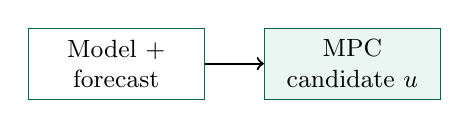
\begin{tikzpicture}[every node/.style={font=\small,align=center},b/.style={draw=forest,text width=2cm,minimum height=.9cm}]
\node[b] (m) {Model +\\forecast};\node[b,fill=mint!25] (u) at (3,0) {MPC\\candidate $u$};\draw[->,thick] (m)--(u);
\end{tikzpicture}\end{center}
Optimization occurs at decision time. A wrong forecast or missing constraint can invalidate the proposal.
\column{.48\textwidth}
\uncover<2->{\textbf{Model-free: learn, then infer}
\begin{center}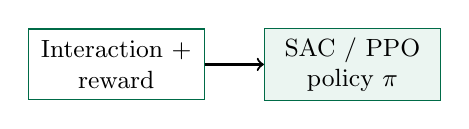
\begin{tikzpicture}[every node/.style={font=\small,align=center},b/.style={draw=forest,text width=2cm,minimum height=.9cm}]
\node[b] (m) {Interaction +\\reward};\node[b,fill=mint!25] (u) at (3,0) {SAC / PPO\\policy $\pi$};\draw[->,thick] (m)--(u);
\end{tikzpicture}\end{center}
Training occurs before use. A new observation produces an action quickly; distribution shift can make it poor.}
\end{columns}
\par\medskip
\small $u$: proposed control; $\pi$: learned observation-to-action rule. SAC is executed here; PPO is a discussed continuous-action alternative.
\par\medskip
\uncover<3->{\textbf{Fair comparison:} same scenario, objective and acceptance limits. Both proposals return to a fresh power-flow check; an LLM response does not replace that check.}

\slidetransition{How does a planner use a forecast before acting?}
\sources{Rawlings, Mayne \& Diehl, \href{https://sites.engineering.ucsb.edu/~jbraw/mpc/}{Model Predictive Control (2017)}. Haarnoja et al., \href{https://proceedings.mlr.press/v80/haarnoja18b.html}{SAC, ICML 2018}; Schulman et al., \href{https://arxiv.org/abs/1707.06347}{PPO (2017)}.}
\note{42--44 min. Model-free describes how the policy is learned, not an absence of engineering models in the full system. The SAC actor was trained using a simulator. PPO can represent continuous actions but is not the trained actor used in this experiment. Keep inference latency distinct from training cost. Spoken bridge: How does a planner use a forecast before acting?}
\end{frame}

\begin{frame}[t]{MPC plans several moves and applies only the first}

\small\textbf{Read the symbols first:} $x_k$ is state, $u_k$ is control and $d_k$ is forecast demand at step $k$. $H$ is the look-ahead horizon; $\ell$ scores one step; $\gamma=0.98$ discounts later steps.
\uncover<2->{\[
\min_{u_0,\ldots,u_{H-1}}\ \underbrace{\sum_{k=0}^{H-1}\gamma^k\ell(x_k,u_k)}_{\text{cost of the proposed sequence}}
\quad\text{s.t.}\quad
\underbrace{x_{k+1}=f(x_k,u_k,d_k)}_{\text{prediction model}},\quad
\underbrace{g(x_k,u_k)\leq0}_{\text{allowed operating region}}.
\]}
\begin{center}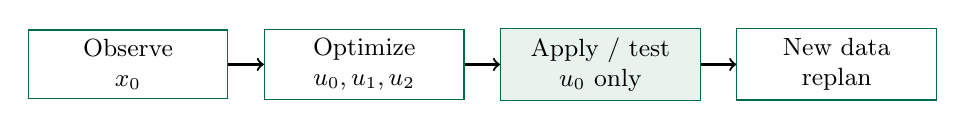
\begin{tikzpicture}[every node/.style={font=\small,align=center},b/.style={draw=forest,text width=2.3cm,minimum height=.8cm}]
\node[b] (a) at (0,0) {Observe\\$x_0$};\node[b] (b) at (3,0) {Optimize\\$u_0,u_1,u_2$};
\node[b,fill=mint!30] (c) at (6,0) {Apply / test\\$u_0$ only};\node[b] (d) at (9,0) {New data\\replan};
\uncover<3->{\draw[->,thick] (a)--(b);\draw[->,thick] (b)--(c);\draw[->,thick] (c)--(d);}
\end{tikzpicture}\end{center}
\uncover<3->{\small\textbf{Our implementation:} $H=3$ quasi-static power-flow snapshots linked by control-movement cost. The generic dynamic equation explains MPC; the tutorial uses algebraic snapshots and does not demonstrate transient stability or a closed-loop rollout.}

\slidetransition{What exactly should one control move minimize?}
\sources{Rawlings, Mayne \& Diehl, \href{https://sites.engineering.ucsb.edu/~jbraw/mpc/}{Model Predictive Control (2017)}.}
\note{44--46 min. Derive receding horizon verbally before showing code. Ask which future action is actually used now. The generalized dynamic equation explains MPC, while the actual tutorial uses algebraic power-flow solves at each forecast step. No terminal-set or closed-loop stability guarantee is claimed. Spoken bridge: What exactly should one control move minimize?}
\end{frame}

\begin{frame}[t]{Make the objective interpretable before optimizing it}

\small\textbf{One two-number fleet command:} $u=(a,b)$. For inverter $i$, $S_i$ is its kVA rating, $a$ is active participation and signed $b$ is reactive participation; both are dimensionless. The one-step teaching cost is $\ell$.
\[
p_i=aS_i,\qquad q_i=bS_i,\qquad b<0\ \Rightarrow\ \text{reactive absorption}.
\]
\uncover<2->{\[
\ell=\underbrace{(1-a)^2}_{\text{unused active capability}}
+\underbrace{0.05b^2}_{\text{reactive effort}}
+\underbrace{10\,\operatorname{mean}[(V-1.01)^2]}_{\text{voltage deviation}}
+\underbrace{0.05\|u-u_{\rm prev}\|_2^2}_{\text{command movement}}.
\]}
\small $V$: modeled voltage magnitudes (p.u.); $1.01$: reference (p.u.); $u_{\rm prev}$: previous command. Model scope determines which voltages enter the mean.
\par\medskip
\textcolor{forest}{\textbf{Predict:}} If we reduce $|b|$, which term certainly decreases? Does total cost necessarily decrease?
\uncover<3->{\par\medskip\textbf{Only the reactive-effort term certainly decreases.} Voltage, movement cost and feasibility can change too. These weights are teaching preferences under the declared availability assumption. A smaller one-step $\ell$ does not establish stability or field performance.}

\slidetransition{Which constraints can overrule a low cost?}
\sources{Actual recorded voltage pilot: \texttt{LLM\_Response\_Selection.ipynb}, E1--E8; raw calls and numerical records in \texttt{results/ensemble\_voltage\_pilot/}.}
\note{46--48 min. Define every symbol; no one should infer the sign convention. The supplied available active power equals the inverter kVA assumption verified in the adapter. The policy does not choose 930 independent inverter settings. Ask: if we reduce reactive effort, can voltage constraints become worse even though one cost term improves? Yes. Spoken bridge: Which constraints can overrule a low cost?}
\end{frame}

\begin{frame}[t]{A low objective is useful only inside the admissible set}

\small\textbf{Symbols before limits:} $V_i$ is bus-phase voltage; $I_e$ is branch current; lower/upper bounds define the contract. $a,b$ are the fleet command; $S_i$ is inverter rating.
\begin{columns}[T]
\column{.48\textwidth}
\uncover<2->{\textbf{Network admissibility}
\[V_{\min}\leq|V_i|\leq V_{\max},\quad |I_e|\leq I_e^{\max}.\]
\textbf{Device admissibility}
\[a^2+b^2\leq1,\quad 0\leq a\leq1,\quad b_{\min}\leq b\leq b_{\max}.\]
The circle follows from $p_i^2+q_i^2\leq S_i^2$.}
\column{.48\textwidth}
\uncover<2->{\textbf{Evidence admissibility}\par
Finite inputs and solver completion; dispatch tracking; matching case, control, model and evidence IDs.
\par\medskip
The planner uses local sensitivities and a conservative capability polygon. The proposed action then returns to the selected numerical model.}
\end{columns}
\par\medskip
\textcolor{forest}{\textbf{Predict:}} Can a majority vote make an excessive current acceptable?
\uncover<3->{\par\textbf{No.} Voting selects a trial. The engineering gate determines whether it can be retained.}

\slidetransition{Which constraints can our chosen model see?}
\sources{Actual recorded voltage pilot: \texttt{LLM\_Response\_Selection.ipynb}, E1--E8; raw calls and numerical records in \texttt{results/ensemble\_voltage\_pilot/}. Rawlings, Mayne \& Diehl, \href{https://sites.engineering.ucsb.edu/~jbraw/mpc/}{Model Predictive Control (2017)}.}
\note{48--50 min. Show the question before revealing. Explain why solver convergence, good objective and feasibility are three different statements. Constants such as voltage bounds and current derating must come from the selected experiment contract, never from generated prose. The local optimizer can be suboptimal; fresh checking is essential. Spoken bridge: Which constraints can our chosen model see?}
\end{frame}

\begin{frame}[t]{LinDistFlow3 and OpenDSS expose different parts of this feeder}

\small
\begin{tabular}{@{}>{\raggedright\arraybackslash}p{.23\linewidth}>{\raggedright\arraybackslash}p{.34\linewidth}>{\raggedright\arraybackslash}p{.35\linewidth}@{}}
\toprule & \textbf{Python LinDistFlow3} & \textbf{OpenDSS} \\
\midrule
Relation & Linear three-phase approximation. & Nonlinear unbalanced power flow. \\
Network & MV; ideal aggregated LV demand. & Supplied MV/LV and transformers. \\
Meaning of PASS & Within the reduced contract. & Within the full-feeder snapshot contract. \\
\bottomrule
\end{tabular}\par
\par\smallskip
\uncover<2->{\textbf{Decode the voltage-drop model:} $\mathbf w_i$ is squared phase voltage at parent bus $i$ (V$^2$); $j$ is its child; $Z_{ij}$ is coupled impedance ($\Omega$); $\mathbf S_{ij}$ is downstream phase power (VA).}
\uncover<3->{\[
\mathbf w_j=\underbrace{\mathbf w_i}_{\text{upstream voltage}}
-\underbrace{2\operatorname{Re}\!\left[\overline\beta\odot\left(Z_{ij}(\beta\odot\overline{\mathbf S}_{ij})\right)\right]}_{\text{three-phase coupled voltage drop}}.
\]
\scriptsize $\beta=(1,e^{-j2\pi/3},e^{-j4\pi/3})$ gives nominal phase ratios; here $j$ in the exponential is the imaginary unit. Bars mean conjugation; $\odot$ means entrywise multiplication; $\operatorname{Re}$ takes the real part.}
\par\smallskip
\uncover<3->{\small\textbf{Comparison boundary:} different network coverage also changes which constraints can fail. This is not an accuracy-only comparison of equivalent models.}

\slidetransition{How does a learned actor produce an alternative?}
\sources{Gan \& Low, \href{https://arxiv.org/abs/1406.3054}{three-phase distribution optimization (2014)}; \href{https://opendss.epri.com/}{EPRI OpenDSS documentation}; \texttt{src/lindistflow3.py}.}
\note{50--52 min. Do not treat agreement of two differently scoped models as a pure accuracy benchmark. The equation matches the fixed-phase phasor closure in src/lindistflow3.py. Mutual impedance coupling is retained. Currents use the fixed 1.03-pu reference; losses are diagnostic and are omitted from the branch balance. Model fidelity and constraint coverage are separate experimental factors. Spoken bridge: How does a learned actor produce an alternative?}
\end{frame}

\begin{frame}[t]{SAC learns a continuous proposal; verification remains a separate step}

\small\textbf{Learning vocabulary:} $s_t$ is an observation, $u_t$ an action, $r$ a reward and $\pi$ the actor. $\mathcal H$ measures policy entropy; $\alpha$ weights exploration and $\gamma$ discounts later rewards.
\uncover<2->{\[
\max_{\pi}\ \mathbb E\!\left[\sum_{t\geq0}\gamma^t
\left\{\underbrace{r(s_t,u_t)}_{\text{task reward}}+\underbrace{\alpha\,\mathcal H(\pi(\cdot\mid s_t))}_{\text{exploration incentive}}\right\}\right].
\]}
\begin{center}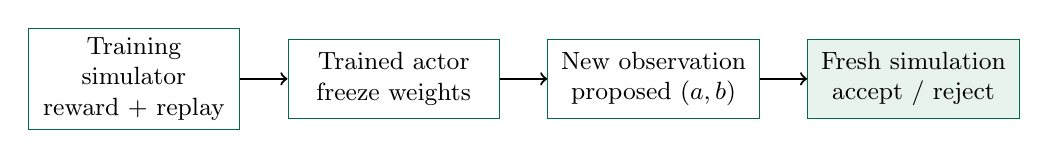
\begin{tikzpicture}[every node/.style={font=\small,align=center},b/.style={draw=forest,text width=2.45cm,minimum height=1cm}]
\node[b] (a) at (0,0) {Training simulator\\reward + replay};\node[b] (b) at (3.3,0) {Trained actor\\freeze weights};
\node[b] (c) at (6.6,0) {New observation\\proposed $(a,b)$};\node[b,fill=mint!30] (d) at (9.9,0) {Fresh simulation\\accept / reject};
\uncover<2->{\draw[->,thick] (a)--(b);\draw[->,thick] (b)--(c);}\uncover<3->{\draw[->,thick] (c)--(d);}
\end{tikzpicture}\end{center}
\uncover<3->{\small\textbf{Executed artifact:} 12,000 training transitions on a cubic surrogate fitted to 240 AC solves; 48 separate fit-validation samples. New scenarios change current-rating conditions: this is transfer, not retraining. A reward penalty does not prove constraint satisfaction.}

\slidetransition{What changes when we perturb the demand?}
\sources{Haarnoja et al., \href{https://proceedings.mlr.press/v80/haarnoja18b.html}{SAC, ICML 2018}; Schulman et al., \href{https://arxiv.org/abs/1707.06347}{PPO (2017)}. Trained artifact: \texttt{Continuous\_SAC\_Training.ipynb}.}
\note{52--53 min. Keep this to one minute; detailed actor and critic training go to the appendix. SAC and the LLM-response selector solve different learning problems. The classroom performs fresh inference with the saved actor weights and freshly checks the action. It does not retrain SAC. The archived training environment uses a fitted cubic surrogate rather than 12,000 full power-flow solves. Spoken bridge: What changes when we perturb the demand?}
\end{frame}

\begin{frame}[t]{Lab 2: change demand and compare the same two numerical actions}

\checkpoint{L2}{Fresh MPC solve, saved-actor inference and fresh numerical checks.}
\cellcode{L2}{1}{5}
\uncover<2->{\exercise{7}{Before running, predict whether a demand change increases PV curtailment or reduces it. Run the default experiment, then change one load multiplier. Compare objective, voltage/current margins and the gate result.}
\textbf{Record three things:} the assumption you changed; the numerical response; whether the original recommendation still has matching evidence.}
\par\smallskip\par
\textbf{Do not infer:} an action that was good at the original load is still good after the change.

\slidetransition{Which margins explain the numerical result?}
\sources{Executed classroom experiment: \texttt{Classroom\_Labs.ipynb}; source: \texttt{src/classroom\_labs.py}. Teaching assumptions are explicit. Rawlings, Mayne \& Diehl, \href{https://sites.engineering.ucsb.edu/~jbraw/mpc/}{Model Predictive Control (2017)}.}
\note{53--60 min. Allow seven minutes including questions. Run L2 as a full cell. Students work in pairs: one predicts, one executes. Ask them to point to a metric supporting their answer. If local setup fails, use the executed output and edit the prediction worksheet rather than waiting for installs. Spoken bridge: Which margins explain the numerical result?}
\end{frame}

\begin{frame}[t]{Read the margins before deciding which controller was better}

\begin{center}\includegraphics[width=.97\linewidth,height=.50\textheight,keepaspectratio]{\figfile{classroom_voltage.png}}\end{center}
\small
\uncover<2->{\textbf{Compare in this order:} did the action pass the same gate? What objective did it achieve? What changed when the demand changed? What was excluded by the model?}
\par\medskip\par
\uncover<3->{\textbf{Bridge:} the numerical methods produced evidence. Now the LLM may choose a bounded next trial from that evidence.}

\slidetransition{What can a language model add to this evidence?}
\sources{Executed classroom experiment: \texttt{Classroom\_Labs.ipynb}; source: \texttt{src/classroom\_labs.py}. Teaching assumptions are explicit.}
\note{60--63 min. This figure is generated by the default L2 execution, not invented to favor agentic AI. A proposal can be feasible but much worse on cost. Ask whether the result comes from MPC, SAC, a better model or orchestration. Keep causal attribution separate. Spoken bridge: What can a language model add to this evidence?}
\end{frame}

\begin{frame}[t]{Actual Llama responses can be useful and still contain unsupported claims}

\small\vspace{.10cm}
\begin{tabular}{@{}>{\raggedright\arraybackslash}p{.18\linewidth}>{\raggedright\arraybackslash}p{.24\linewidth}>{\raggedright\arraybackslash}p{.48\linewidth}@{}}
\toprule Model / time & Selected trial & Excerpt from its recorded public response \\
\midrule
Llama 3.1 8B\newline 1.867 s & Increase $a$ by 0.0025 & ``Increasing active participation by 0.0025 may help reduce curtailment and improve the overall performance.'' \\
Llama 3.2 3B\newline 0.905 s & Reduce $|b|$ by 10\% & ``Reducing reactive effort magnitude by ten percent may help improve the overall system performance and reduce curtailment'' \\
Qwen 2.5 7B\newline 1.844 s & Reduce $|b|$ by 10\% & ``may help improve voltage stability without significantly degrading active power performance'' \\
\bottomrule
\end{tabular}\par
\par\medskip
\checkpoint{L3}{Original archived test 01; separate from the changed L2 classroom case.}
\uncover<2->{\textbf{Critique:} less reactive effort alone does not establish less curtailment. These steady-state tests do not establish voltage stability.}

\slidetransition{How do different replies become comparable actions?}
\sources{Actual recorded voltage pilot: \texttt{LLM\_Response\_Selection.ipynb}, E1--E8; raw calls and numerical records in \texttt{results/ensemble\_voltage\_pilot/}.}
\note{63--68 min. Run L3 and allow students to identify one supported and one unsupported clause before revealing. These are short exact excerpts; full public responses are in the notebook. They are not private chain-of-thought. Actual times were recorded in September, not measured by the new cached display cell. Llama is the model family; Ollama is the local runtime. Spoken bridge: How do different replies become comparable actions?}
\end{frame}

\begin{frame}[t]{Voting selects one physical operation, not the most persuasive paragraph}

\begin{center}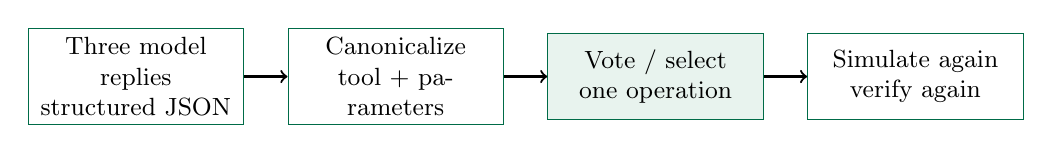
\begin{tikzpicture}[every node/.style={font=\small,align=center},b/.style={draw=forest,text width=2.5cm,minimum height=1.1cm}]
\node[b] (a) at (0,0) {Three model replies\\structured JSON};\node[b] (b) at (3.3,0) {Canonicalize\\tool + parameters};
\node[b,fill=mint!30] (c) at (6.6,0) {Vote / select\\one operation};\node[b] (d) at (9.9,0) {Simulate again\\verify again};
\draw[->,thick] (a)--(b);\draw[->,thick] (b)--(c);\draw[->,thick] (c)--(d);
\end{tikzpicture}\end{center}
\par\medskip
Two descriptions of the same $(a,b)$ should not become two different actions. Canonical IDs make duplicates and ties reproducible.
\par\medskip
\uncover<2->{\textbf{Test 01:} two models propose the same Q reduction; one proposes a PV increase. The majority selects the Q trial.}
\par\medskip
\uncover<3->{\textbf{Why disagreement matters:} it suggests another candidate to test. It does not quantify the probability that the grid action is safe.}

\slidetransition{Can feedback teach us which operation to test?}
\sources{Actual recorded voltage pilot: \texttt{LLM\_Response\_Selection.ipynb}, E1--E8; raw calls and numerical records in \texttt{results/ensemble\_voltage\_pilot/}. Ensemble evaluation context: \href{https://arxiv.org/abs/2606.18789}{PowerAgentBench-SS (2026)}.}
\note{68--70 min. Explain that a predetermined SHA tie-break is repeatability, not engineering preference. Correlated models can share a mistaken assumption. The all-responses comparator receives more numerical trials and must be labeled as extra budget. Voting cannot lower limits or invent permissions. Spoken bridge: Can feedback teach us which operation to test?}
\end{frame}

\begin{frame}[t]{The LLM optimizer can learn which proposed operation to test}

\small\textbf{Select $\rightarrow$ observe $\rightarrow$ update.} Here $s$ is the evidence summary and $a$ is a canonical proposed operation. $\phi(s,a)$ encodes their features; $\theta$ stores learned reward coefficients; $A$ stores regularized feature information; $\beta$ weights exploration. Score $q$ chooses the next operation $a^*$.
\uncover<2->{\[
q(a\mid s)=\underbrace{\theta^\top\phi(s,a)}_{\text{predicted reward}}
+\underbrace{\beta\sqrt{\phi(s,a)^\top A^{-1}\phi(s,a)}}_{\text{training exploration bonus}},
\qquad a^*=\arg\max_a q(a\mid s).
\]}
\uncover<3->{\small After selection, observe reward $r$ and update $A$ and reward vector $b$:
\[
A\leftarrow A+\phi\phi^\top,\qquad b\leftarrow b+r\phi,\qquad\theta=A^{-1}b.
\]
This reward vector $b$ is unrelated to inverter $b$. Frozen L4 evaluation uses predicted reward only, without updates.}
\par\smallskip
\checkpoint{L4}{Load the frozen LinUCB selector, choose an operation and recheck it.}
\textbf{Boundary:} the bandit selects among already generated responses. It neither selects which LLM to call nor trains LLM weights.

\slidetransition{What reward should the selector receive?}
\sources{Li et al., \href{https://arxiv.org/abs/1003.0146}{LinUCB, WWW 2010}; Actual recorded voltage pilot: \texttt{LLM\_Response\_Selection.ipynb}, E1--E8; raw calls and numerical records in \texttt{results/ensemble\_voltage\_pilot/}.}
\note{70--73 min. First describe select, observe, update in words. Then reveal the equations. Training has an uncertainty bonus; frozen classroom evaluation uses predicted reward only. The selected-feedback simulator replay is not observational deployment data. No future score, gate outcome or held-out feedback may enter selection features. Spoken bridge: What reward should the selector receive?}
\end{frame}

\begin{frame}[t]{Reward learning and safety checking have different jobs}

\small $J_{\rm inc}$ and $J_{\rm trial}$ are incumbent and trial current-step costs; $r$ is feedback after a numerical trial.
\uncover<2->{\[
r=\begin{cases}
\min(1,\max(0,J_{\rm inc}-J_{\rm trial})/0.01)-0.01,&\text{trial passes},\\
-1.01,&\text{trial rejected}.
\end{cases}
\]}
\small The penalty 0.01 is a fixed trial charge, not latency in seconds.
\par\medskip
\textbf{Learning design:} 24 training contexts, 8 validation, 12 test; five training orders over the same data. Frozen validation/test: zero updates.
\par\medskip
\exercise{3}{Run L4. Compare the selected trial with the majority vote. If the reward predicts improvement but fresh verification fails, which result should control the recommendation?}
\uncover<3->{\textbf{The gate.} Retain a valid incumbent or escalate. Reward optimization does not create an operating permission.}

\slidetransition{Does the learned selector outperform a simpler rule?}
\sources{Actual recorded voltage pilot: \texttt{LLM\_Response\_Selection.ipynb}, E1--E8; raw calls and numerical records in \texttt{results/ensemble\_voltage\_pilot/}. Executed classroom experiment: \texttt{Classroom\_Labs.ipynb}; source: \texttt{src/classroom\_labs.py}. Teaching assumptions are explicit.}
\note{73--76 min. Reserve the three minutes. Training and test files are separate. All permitted trial outcomes exist for audit, but training consumes only selected feedback. Ask how changing the reward scaling changes learning without changing the physical limits. The posthoc simple-rule diagnostic is not a predeclared baseline. Spoken bridge: Does the learned selector outperform a simpler rule?}
\end{frame}

\begin{frame}[t]{A rigorous result can show that the extra agent adds no benefit}

\begin{tabular}{@{}lrrr@{}}
\toprule MV test, 12 scenarios & Mean $J$ & Full-feeder AC PASS & Accounted time \\
\midrule
Numerical fixed refinement & 0.03400656 & 0/12 & 3.327 s \\
Majority vote & 0.03398479 & 0/12 & Pool cost applies \\
Learned selector & 0.03398479 & 0/12 & 8.119 s \\
\bottomrule
\end{tabular}\par
\par\medskip
\uncover<2->{Learned selection and voting tie on every held-out case. A posthoc fixed Q-reduction rule also reproduces these decisions without LLM calls.}
\par\medskip
\uncover<3->{\textbf{What is demonstrated?} Reproducible proposals, traceable refinement and explicit model-scope checking.
\par\medskip
\textbf{What is not demonstrated?} Superior control from extra LLMs or learning. A simpler supervisor is a serious comparator.}

\slidetransition{Will the same action pass a broader model?}
\sources{Actual recorded voltage pilot: \texttt{LLM\_Response\_Selection.ipynb}, E1--E8; raw calls and numerical records in \texttt{results/ensemble\_voltage\_pilot/}.}
\note{76--78 min. Do not hide the negative result. The denominator is 12 scenarios, not number of model calls. The measured time is reconstructed serial accounting from actual components. A claim that agentic AI improves optimization must survive the identical-tool fixed-rule baseline. Explain why this negative result is a valuable research lesson. Spoken bridge: Will the same action pass a broader model?}
\end{frame}

\begin{frame}[t]{Lab 5: ask a broader model to audit the recommendation}

\checkpoint{L5}{Fresh MV check; optional fresh AC audit and separate AC replanning.}
\cellcode{L5}{1}{5}
\uncover<2->{\small\textbf{Separate recorded pilot: 12 paired cases}\par\smallskip\begin{tabular}{@{}>{\raggedright\arraybackslash}p{.38\linewidth}rr@{}}
\toprule Final learned-workflow result & MV planning & OpenDSS planning \\
\midrule
Selected-model final checks & 12/12 & 12/12 \\
Full-feeder AC checks & 0/12 & 12/12 \\
Human operating approval & Pending & Pending \\
\bottomrule
\end{tabular}\par}
\par\medskip
\uncover<3->{\textbf{Causal explanation:} the network coverage and acceptance contract changed. The learned selector remained frozen. Do not attribute the broader-model benefit to Llama.}

\slidetransition{Which stage produced each part of the evidence?}
\sources{Actual recorded voltage pilot: \texttt{LLM\_Response\_Selection.ipynb}, E1--E8; raw calls and numerical records in \texttt{results/ensemble\_voltage\_pilot/}. Executed classroom experiment: \texttt{Classroom\_Labs.ipynb}; source: \texttt{src/classroom\_labs.py}. Teaching assumptions are explicit.}
\note{78--80 min. Default performs a fresh MV audit of the archived original action. If OpenDSS is installed, enable the fresh AC check and separate AC replanning. The 12-case table on this slide is the separately labeled historical pilot, not output from this one-case cell. Both audiences use the same tool contract. Explain that different bus sets also change the voltage term in the objective, so cross-model objective values are not a pure solver ranking. Spoken bridge: Which stage produced each part of the evidence?}
\end{frame}

\begin{frame}[t]{Voltage support: what each stage contributed}

\small
\begin{center}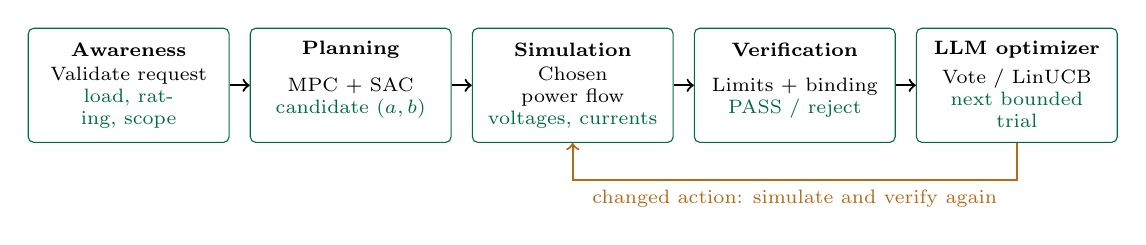
\begin{tikzpicture}[every node/.style={font=\scriptsize,align=center},b/.style={draw=forest,rounded corners=2pt,text width=2.34cm,minimum height=1.45cm,inner sep=3pt}]
\node[b] (a) at (0,0) {};
\node[font=\scriptsize\bfseries] at ([yshift=.45cm]a.center) {Awareness};
\uncover<1->{\node[text width=2.22cm] at ([yshift=-.16cm]a.center) {Validate request\\\textcolor{forest}{load, rating, scope}};}
\node[b] (p) at (2.82,0) {};
\node[font=\scriptsize\bfseries] at ([yshift=.45cm]p.center) {Planning};
\uncover<1->{\node[text width=2.22cm] at ([yshift=-.16cm]p.center) {MPC + SAC\\\textcolor{forest}{candidate $(a,b)$}};}
\node[b] (s) at (5.64,0) {};
\node[font=\scriptsize\bfseries] at ([yshift=.45cm]s.center) {Simulation};
\uncover<2->{\node[text width=2.22cm] at ([yshift=-.16cm]s.center) {Chosen power flow\\\textcolor{forest}{voltages, currents}};}
\node[b] (v) at (8.46,0) {};
\node[font=\scriptsize\bfseries] at ([yshift=.45cm]v.center) {Verification};
\uncover<2->{\node[text width=2.22cm] at ([yshift=-.16cm]v.center) {Limits + binding\\\textcolor{forest}{PASS / reject}};}
\node[b] (o) at (11.28,0) {};
\node[font=\scriptsize\bfseries] at ([yshift=.45cm]o.center) {LLM optimizer};
\uncover<3->{\node[text width=2.22cm] at ([yshift=-.16cm]o.center) {Vote / LinUCB\\\textcolor{forest}{next bounded trial}};}
\draw[->,thick] (a)--(p);\draw[->,thick] (p)--(s);\draw[->,thick] (s)--(v);\draw[->,thick] (v)--(o);
\uncover<3->{\draw[->,thick,orange] (o.south)--(11.28,-1.2)--node[below,font=\scriptsize]{changed action: simulate and verify again}(5.64,-1.2)--(s.south);}
\end{tikzpicture}\end{center}
\textbf{Evidence provenance:} L2 performs fresh numerical solves and saved-actor inference. L3--L5 separately inspect the recorded response-selection pilot; its Llama replies are archived.
\par\medskip
\uncover<4->{\textbf{Operator handoff:} retain the checked action, model scope and failed limits. In the recorded test, voting and learned selection tie; the reduced-model actions still fail the broader AC audit. The architecture exposes this boundary rather than proving better control.}

\slidetransition{What changes when the decision is a topology, not a setpoint?}
\sources{Executed classroom experiment: \texttt{Classroom\_Labs.ipynb}; source: \texttt{src/classroom\_labs.py}. Teaching assumptions are explicit. Actual recorded voltage pilot: \texttt{LLM\_Response\_Selection.ipynb}, E1--E8; raw calls and numerical records in \texttt{results/ensemble\_voltage\_pilot/}.}
\note{80--82 min. Ask one participant to summarize the actual benefit and one limitation. The language layer provides bounded interpretation and trial selection; engineering methods produce the physical evidence. Transition to topology and discrete optimization. This completes voltage without switching to another historical protocol mid-lesson. Spoken bridge: What changes when the decision is a topology, not a setpoint?}
\end{frame}

\begin{frame}{Ten-minute break: 82--92 minutes}
\centering\Large Keep the notebook kernel running.\par\bigskip
\normalsize We have adjusted controls on a fixed network.\par\medskip
Next: a fault changes the available paths.\par\medskip
Which loads should the remaining network support?
\slidetransition{After the break, which loads should the remaining paths support?}
\sources{Workshop timing: ten full minutes; no required work during the break.}
\note{82--92 minutes. Take the full break. Resume at restoration. This frame is inside the taught route; appendix material must not consume the break.}
\end{frame}
\section{Restoration}
\begin{frame}[t]{After a fault, reconnecting service is a discrete decision}

\begin{center}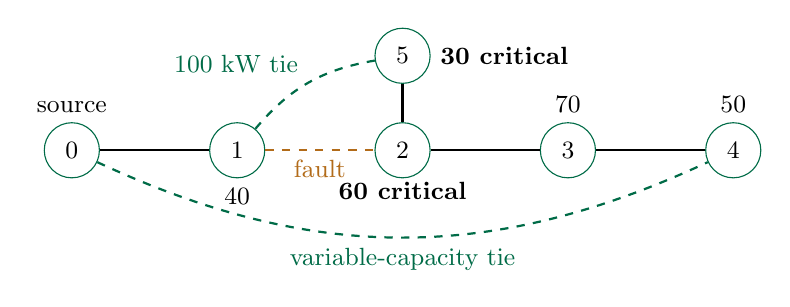
\begin{tikzpicture}[x=2.1cm,y=.8cm,every node/.style={font=\small},n/.style={circle,draw=forest,minimum size=7mm}]
\node[n] (a) at (0,0) {0};\node[n] (b) at (1,0) {1};\node[n] (c) at (2,0) {2};\node[n] (d) at (3,0) {3};\node[n] (e) at (4,0) {4};\node[n] (f) at (2,1.5) {5};
\draw[thick] (a)--(b);\draw[thick,orange,dashed] (b)--node[below]{fault}(c);\draw[thick] (c)--(d)--(e);\draw[thick] (c)--(f);
\uncover<2->{\draw[thick,forest,dashed] (b) to[bend left=20] node[above left]{100 kW tie} (f);
\draw[thick,forest,dashed] (a) to[bend right=25] node[below]{variable-capacity tie} (e);}
\node[above] at (a.north) {source};\node[below] at (b.south) {40};\node[below,fill=white,inner sep=1pt] at (c.south) {\textbf{60 critical}};\node[above] at (d.north) {70};\node[above] at (e.north) {50};\node[right] at (f.east) {\textbf{30 critical}};
\end{tikzpicture}\end{center}
\small Loads and tie capacities are in kW. This transparent six-node teaching graph is separate from the Greensboro feeder.
\par\medskip\textbf{Predict:} Can bus 4 carry power onward while its own load remains disconnected?
\uncover<3->{\par\medskip\textbf{Yes.} Energizing a bus and picking up its load are different decisions.}

\slidetransition{How do we express pickup, energization and connectivity?}
\sources{Chen et al., \href{https://doi.org/10.1109/TPWRS.2017.2720122}{IEEE TPWRS (2018)}; Wang et al., \href{https://arxiv.org/abs/1912.05185}{radiality constraints (2020)}.}
\note{92--95 min. Resume from the break with a physical question. Draw attention to node 4 as a transit node. Ask for predictions before revealing. The faulted edge is unavailable, not merely expensive. Dashed green ties are choices, not a preselected solution. Spoken bridge: How do we express pickup, energization and connectivity?}
\end{frame}

\begin{frame}[t]{Restoration MILP: choose service while preserving a source path}

\footnotesize\setlength{\abovedisplayskip}{4pt}\setlength{\belowdisplayskip}{4pt}
\textbf{Three binary choices:} $s_i$ picks up load $i$; $y_i$ energizes its bus; $z_e$ closes edge $e$. Demand $d_i$ is in kW; priority $w_i=10$ for critical loads and $1$ otherwise. Source $y_0=1$.
\uncover<2->{\[
\underbrace{\max\sum_i w_i d_i s_i}_{\text{weighted service}},\qquad
\underbrace{s_i\leq y_i,\quad z_{ij}\leq y_i,y_j}_{\text{pickup and edges need energized buses}},\quad z_{\rm fault}=0.
\]}
\uncover<3->{\footnotesize $P_e$ is signed active flow; $\overline P_e$ is edge capacity (kW); $A$ is the node-edge incidence matrix.
\[
\underbrace{\sum_e A_{ie}P_e=d_is_i\quad(i\ne0)}_{\text{power reaches each served load}},\qquad
\underbrace{|P_e|\leq\overline P_ez_e}_{\text{open edge carries no flow}}.
\]}
\uncover<4->{\footnotesize $f_e$ is a fictitious connectivity commodity, not electricity; each energized non-source bus consumes one unit.
\[
\sum_e A_{ie}f_e=y_i\ (i\ne0),\qquad |f_e|\leq5z_e,\qquad
\underbrace{\sum_ez_e=\sum_i y_i-1}_{\text{connectivity + edge count gives a tree}}.
\]
\textbf{Scope:} six-node active-power transport model; AC voltage, reactive power and switching chronology are omitted.}

\slidetransition{What makes the comparison with a baseline fair?}
\sources{Chen et al., \href{https://doi.org/10.1109/TPWRS.2017.2720122}{IEEE TPWRS (2018)}; Wang et al., \href{https://arxiv.org/abs/1912.05185}{radiality constraints (2020)}.}
\note{95--99 min. Spend four minutes connecting each equation to the picture. Edge count alone is insufficient. Fictitious flow is a graph certificate, not electricity. The source supplies commodity and electrical balances; non-source equations shown for clarity. The exact model is solved by SciPy/HiGHS and independently enumerated. A secondary solve preserves the optimal weighted service, then minimizes energized branch count plus a 0.001 edge-index tie-break. This is not a count of switching operations relative to an initial topology. Spoken bridge: What makes the comparison with a baseline fair?}
\end{frame}

\begin{frame}[t]{A fair baseline must optimize the same feasible network}

\begin{tabular}{@{}>{\raggedright\arraybackslash}p{.27\linewidth}>{\raggedright\arraybackslash}p{.31\linewidth}>{\raggedright\arraybackslash}p{.33\linewidth}@{}}
\toprule & Unweighted service baseline & Priority-weighted service \\
\midrule
Objective & $\max\sum_i d_i s_i$ & $\max\sum_i w_i d_i s_i$ \\
Same constraints? & \yesmark & \yesmark \\
Same fault / capacities? & \yesmark & \yesmark \\
Exact solution method & Exhaustive enumeration & HiGHS MILP + enumeration check \\
Report & Total and critical kW & Total and critical kW \\
\bottomrule
\end{tabular}\par
\par\medskip
\uncover<2->{\textbf{Interpretation:} a difference caused by priority weights is an optimization-policy effect. It is not evidence that an LLM discovered a better optimizer.}
\par\medskip
\uncover<3->{\textbf{Agent opportunity:} turn a documented priority instruction into a validated parameter change; preserve the fault exclusions, action permissions and evidence chain.}

\slidetransition{Where should the service curve change as capacity shrinks?}
\sources{Chen et al., \href{https://doi.org/10.1109/TPWRS.2017.2720122}{IEEE TPWRS (2018)}; Wang et al., \href{https://arxiv.org/abs/1912.05185}{radiality constraints (2020)}. Executed classroom experiment: \texttt{Classroom\_Labs.ipynb}; source: \texttt{src/classroom\_labs.py}. Teaching assumptions are explicit.}
\note{99--102 min. The new lab baseline solves the same constraints with unit weights. It is stronger and clearer than an arbitrary greedy ordering. Finite weight ten is not a universal lexicographic priority guarantee. Ask how to implement strict critical-first priority: solve two stages or impose a verified primary objective bound. Spoken bridge: Where should the service curve change as capacity shrinks?}
\end{frame}

\begin{frame}[t]{Lab 6: predict the effect of reducing tie capacity}

\checkpoint{L6}{Fresh capacity sweep; independent enumeration checks the MILP.}
\cellcode{L6}{1}{5}
\uncover<2->{\exercise{8}{Predict total and critical service at 40, 60, 80 and 120 kW. Run the sweep; add a tighter rating. Compare weighted and unweighted solutions. Explain a flat region in the service curve.}
\textbf{Inspect:} picked-up loads, closed edges, critical kW, total kW and enumeration agreement.}
\par\smallskip\par
\textbf{Why a sweep?} One attractive topology cannot show how priorities and constraints interact.

\slidetransition{Why can several ratings produce the same service?}
\sources{Executed classroom experiment: \texttt{Classroom\_Labs.ipynb}; source: \texttt{src/classroom\_labs.py}. Teaching assumptions are explicit. Chen et al., \href{https://doi.org/10.1109/TPWRS.2017.2720122}{IEEE TPWRS (2018)}; Wang et al., \href{https://arxiv.org/abs/1912.05185}{radiality constraints (2020)}.}
\note{102--110 min. Includes the beginning of the restoration lab block. Pair exercise: one follows the source path, one checks branch capacities. Do not infer proportional service reduction from proportional capacity reduction. If ties occur, compare objective and feasibility rather than insisting on identical edge IDs. Spoken bridge: Why can several ratings produce the same service?}
\end{frame}

\begin{frame}[t]{Discrete service can stay constant while a rating changes}

\begin{center}\includegraphics[width=.97\linewidth,height=.51\textheight,keepaspectratio]{\figfile{classroom_restoration.png}}\end{center}
\small
\uncover<2->{\textbf{Explain the sampled service levels:} loads are indivisible in this model. A tighter rating changes the solution only when it excludes a useful feasible pickup pattern.}
\par\medskip\par
\uncover<3->{\textbf{At 100 and 80 kW in the priority formulation:} 200 kW total, 90 kW critical. Bus 4 may remain energized while its own load is disconnected.}

\slidetransition{Can this result still be used after the topology changes?}
\sources{Executed classroom experiment: \texttt{Classroom\_Labs.ipynb}; source: \texttt{src/classroom\_labs.py}. Teaching assumptions are explicit.}
\note{110--113 min. Plot is generated from fresh solves. Ask students to locate a capacity at which the two objectives favor different critical service, if such a point appears in the executed sweep. A tie is also an informative result; do not invent a benefit. Review one selected branch-flow constraint numerically. Spoken bridge: Can this result still be used after the topology changes?}
\end{frame}

\begin{frame}[t]{Lab 7: a changed topology needs a new evidence record}

\checkpoint{L7}{Try to reuse a result after changing the case.}
\cellcode{L7}{7}{10}
\exercise{3}{Change a capacity or pickup request while retaining the old evidence. Predict the verifier outcome. Recompute the evidence and repeat the handoff.}
\par\medskip
\uncover<2->{\textbf{The safeguard:} a passing result is bound to the case, control, model and contract that were actually checked.}
\par\medskip
\uncover<3->{\textbf{The limit:} this cannot establish field isolation, switch availability or protection coordination. Those need separate authorized evidence.}

\slidetransition{Which stage must repair a stale handoff?}
\sources{Executed classroom experiment: \texttt{Classroom\_Labs.ipynb}; source: \texttt{src/classroom\_labs.py}. Teaching assumptions are explicit. State-prerequisite guards: \href{https://arxiv.org/abs/2603.17418}{PowerDAG (2026)}.}
\note{113--116 min. The intended outcome is rejection of stale evidence, not merely producing a warning in prose. Ask which fields should change when the topology changes. This experiment demonstrates a deterministic architectural property available to both fixed and LLM-based supervisors. Spoken bridge: Which stage must repair a stale handoff?}
\end{frame}

\begin{frame}[t]{Use every workflow stage, but attribute the benefit correctly}

\small
\begin{center}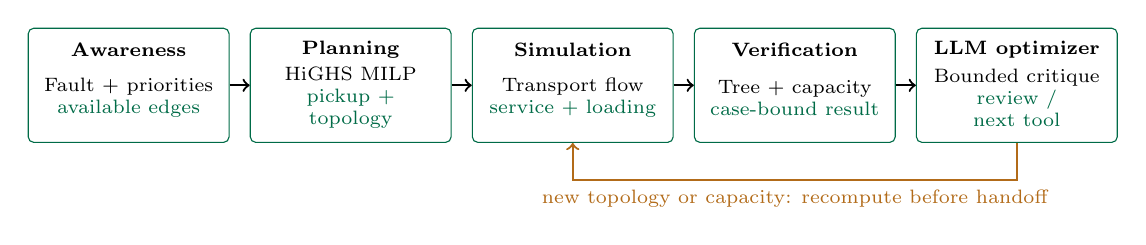
\begin{tikzpicture}[every node/.style={font=\scriptsize,align=center},b/.style={draw=forest,rounded corners=2pt,text width=2.34cm,minimum height=1.45cm,inner sep=3pt}]
\node[b] (a) at (0,0) {};
\node[font=\scriptsize\bfseries] at ([yshift=.45cm]a.center) {Awareness};
\uncover<1->{\node[text width=2.22cm] at ([yshift=-.16cm]a.center) {Fault + priorities\\\textcolor{forest}{available edges}};}
\node[b] (p) at (2.82,0) {};
\node[font=\scriptsize\bfseries] at ([yshift=.45cm]p.center) {Planning};
\uncover<1->{\node[text width=2.22cm] at ([yshift=-.16cm]p.center) {HiGHS MILP\\\textcolor{forest}{pickup + topology}};}
\node[b] (s) at (5.64,0) {};
\node[font=\scriptsize\bfseries] at ([yshift=.45cm]s.center) {Simulation};
\uncover<2->{\node[text width=2.22cm] at ([yshift=-.16cm]s.center) {Transport flow\\\textcolor{forest}{service + loading}};}
\node[b] (v) at (8.46,0) {};
\node[font=\scriptsize\bfseries] at ([yshift=.45cm]v.center) {Verification};
\uncover<2->{\node[text width=2.22cm] at ([yshift=-.16cm]v.center) {Tree + capacity\\\textcolor{forest}{case-bound result}};}
\node[b] (o) at (11.28,0) {};
\node[font=\scriptsize\bfseries] at ([yshift=.45cm]o.center) {LLM optimizer};
\uncover<3->{\node[text width=2.22cm] at ([yshift=-.16cm]o.center) {Bounded critique\\\textcolor{forest}{review / next tool}};}
\draw[->,thick] (a)--(p);\draw[->,thick] (p)--(s);\draw[->,thick] (s)--(v);\draw[->,thick] (v)--(o);
\uncover<3->{\draw[->,thick,orange] (o.south)--(11.28,-1.2)--node[below,font=\scriptsize]{new topology or capacity: recompute before handoff}(5.64,-1.2)--(s.south);}
\end{tikzpicture}\end{center}
\textbf{Evidence provenance:} L6--L7 freshly solve the six-node graph and test stale-evidence rejection. The five-stage Llama example is a separate recorded feeder catalog, inspected in L10.
\par\medskip
\uncover<4->{\textbf{Operator handoff:} review isolation, permissions and model scope. In the recorded feeder comparison, the fixed and Llama routes obtain the same service objective; explanation adds traceability and latency, not demonstrated extra restored load.}

\slidetransition{Can correctly bound evidence still describe the wrong state?}
\sources{Executed classroom experiment: \texttt{Classroom\_Labs.ipynb}; source: \texttt{src/classroom\_labs.py}. Teaching assumptions are explicit. Actual recorded five-stage reference: \texttt{Proposal\_Complete\_Workflow.ipynb}, P1--P8; \texttt{results/proposal\_complete\_workflow.json}.}
\note{116--118 min. Keep the six-node live exercise separate from the archived feeder catalog. The archived actual agent traces can be inspected in L10 later. The language model is not required to solve the MILP. The standard method establishes numerical decisions; the architecture makes handoffs and unsupported assertions inspectable. Spoken bridge: Can correctly bound evidence still describe the wrong state?}
\end{frame}

\begin{frame}[t]{From restoration to cyber response: what if the evidence is wrong?}

\textbf{Established so far}\par
We can optimize a permitted topology and reject evidence that belongs to the wrong case.
\par\medskip
\uncover<2->{\textbf{A harder question}\par
What if the record matches the case, but the measurements inside it are corrupted?}
\uncover<3->{\begin{center}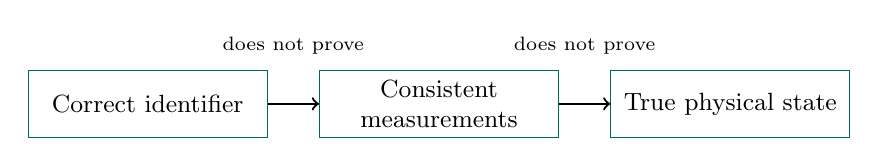
\begin{tikzpicture}[every node/.style={font=\small,align=center},b/.style={draw=forest,text width=2.8cm,minimum height=.85cm}]
\node[b] (a) at (0,0) {Correct identifier};\node[b] (b) at (3.7,0) {Consistent measurements};\node[b] (c) at (7.4,0) {True physical state};
\draw[->,thick] (a)--node[above=5mm,font=\scriptsize]{does not prove}(b);\draw[->,thick] (b)--node[above=5mm,font=\scriptsize]{does not prove}(c);
\end{tikzpicture}\end{center}}
\uncover<3->{\textbf{Next experiment:} construct a measurement error that the usual residual test cannot see, then inspect its control consequence.}

\slidetransition{How does an operator estimate a state from imperfect sensors?}
\sources{Schweppe \& Wildes, \href{https://doi.org/10.1109/TPAS.1970.292678}{state estimation (1970)}; Liu, Ning \& Reiter, \href{https://doi.org/10.1145/1653662.1653666}{false-data injection, CCS 2009}.}
\note{118--119 min. Explicit conceptual bridge. Identity, consistency and truth are different properties. The next case is a four-bus DC model designed to expose this distinction, not an attack on the full Greensboro feeder. Spoken bridge: How does an operator estimate a state from imperfect sensors?}
\end{frame}

\section{Cyber response}
\begin{frame}[t]{Cyber response begins with an estimation problem}

\begin{center}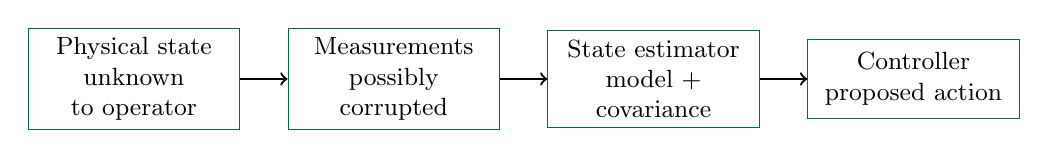
\begin{tikzpicture}[every node/.style={font=\small,align=center},b/.style={draw=forest,text width=2.45cm,minimum height=1cm}]
\node[b] (a) at (0,0) {Physical state\\unknown to operator};\node[b] (b) at (3.3,0) {Measurements\\possibly corrupted};\node[b] (c) at (6.6,0) {State estimator\\model + covariance};\node[b] (d) at (9.9,0) {Controller\\proposed action};
\draw[->,thick] (a)--(b);\draw[->,thick] (b)--(c);\draw[->,thick] (c)--(d);
\end{tikzpicture}\end{center}
\par\medskip
\textbf{Four-bus DC teaching system:} three unknown non-reference voltage angles; eight measurements of flows, injections and one angle.
\par\medskip
\uncover<2->{\textbf{Two cases:} an isolated biased sensor and a coordinated model-consistent perturbation.}
\par\medskip
\uncover<3->{The experimenter knows synthetic truth to score the outcome. The agent's operating gate does not receive that truth.}

\slidetransition{What does a residual actually measure?}
\sources{Schweppe \& Wildes, \href{https://doi.org/10.1109/TPAS.1970.292678}{state estimation (1970)}; Liu, Ning \& Reiter, \href{https://doi.org/10.1145/1653662.1653666}{false-data injection, CCS 2009}.}
\note{119--121 min. Begin from data flow. The teacher knows the simulated state; the controller does not. The attack is confined to this numerical teaching fixture. We are studying limitations of a detector and safe handling of uncertainty, not exploiting infrastructure. Spoken bridge: What does a residual actually measure?}
\end{frame}

\begin{frame}[t]{WLS measures consistency with a model and noise assumption}

\small\textbf{Symbols first:} $x\in\mathbb R^3$ contains unknown angles (rad); $z\in\mathbb R^8$ contains sensor readings; $H$ maps state to measurements. Noise $\epsilon$ has covariance $R$, which weights each sensor in its own units. WLS returns estimate $\hat x$.
\uncover<2->{\[
z=Hx+\epsilon,\quad\epsilon\sim\mathcal N(0,R),\qquad
\hat x=\arg\min_x\underbrace{(z-Hx)^\top R^{-1}(z-Hx)}_{\text{weighted mismatch between readings and model}}.
\]}
\uncover<3->{\small The residual $r$ is the unexplained measurement mismatch; $J$ is its dimensionless weighted energy.
\[
r=z-H\hat x,\qquad J=r^\top R^{-1}r,\qquad
\underbrace{J>\chi^2_{5,0.99}=15.0863}_{\text{five residual degrees of freedom: }8-3}\ \Rightarrow\ \text{alarm}.
\]}
\uncover<4->{\textbf{What this means:} readings inconsistent with the assumed model and noise. It does not identify malicious intent.\par\smallskip
\small The 1\% nominal false-alarm level assumes a correct linear model, Gaussian noise and full observability. It is not a measured field false-alarm rate.}

\slidetransition{Can the estimate change while the residual stays the same?}
\sources{Schweppe \& Wildes, \href{https://doi.org/10.1109/TPAS.1970.292678}{state estimation (1970)}; Liu, Ning \& Reiter, \href{https://doi.org/10.1145/1653662.1653666}{false-data injection, CCS 2009}.}
\note{121--124 min. Solve with weighted least squares rather than explicitly inverting a normal matrix in numerical code. Walk through the meaning of covariance. Full column rank matters before thresholding. An alarm says the readings are inconsistent with the assumptions, not which actor caused the problem. Spoken bridge: Can the estimate change while the residual stays the same?}
\end{frame}

\begin{frame}[t]{A coordinated perturbation can change the estimate without the residual}

\small Define $c$ as a state displacement, $a$ as a measurement perturbation and primes as changed quantities. Choose a coordinated pattern $a=Hc$:
\[
z'=z+Hc.
\]
\uncover<2->{For the same full-rank linear WLS model, $\hat x'=\hat x+c$. Therefore
\[
r'=z'-H\hat x'=z+Hc-H(\hat x+c)=z-H\hat x=r.
\]}
\uncover<3->{\textbf{Same residual, different estimated state.}\par
A controller can confidently choose an action for the wrong operating point. More eloquent interpretation of the same residual does not recover the missing information.}
\par\medskip
\small This construction assumes the attacker can alter the required measurement pattern and knows the relevant linear model. Real restrictions can limit that capability.

\slidetransition{What do the residual and state-error curves look like?}
\sources{Schweppe \& Wildes, \href{https://doi.org/10.1109/TPAS.1970.292678}{state estimation (1970)}; Liu, Ning \& Reiter, \href{https://doi.org/10.1145/1653662.1653666}{false-data injection, CCS 2009}.}
\note{124--128 min. Match the reference teaching style: keep the same equation visible and reveal cancellation step by step. Ask learners to cancel Hc themselves before showing the answer. This is a mathematical negative control, not a claim that all attacks are stealthy or all networks are equally vulnerable. Spoken bridge: What do the residual and state-error curves look like?}
\end{frame}

\begin{frame}[t]{Lab 8: sweep the attack size and watch two different signals}

\checkpoint{L8}{Fresh WLS experiment for isolated and model-consistent perturbations.}
\cellcode{L8}{1}{5}
\uncover<2->{\exercise{7}{Predict the residual and state-error curves for both perturbations. Run the sweep. Find an example where the residual stays below threshold while state error grows.}
\textbf{Keep two plots separate:} a detector sees residual statistics; the experimenter evaluates estimation error using synthetic truth.}
\par\medskip
\textbf{Question:} what can the agent truthfully conclude from ``no residual alarm''?

\slidetransition{Which plotted signal is available to the operator?}
\sources{Executed classroom experiment: \texttt{Classroom\_Labs.ipynb}; source: \texttt{src/classroom\_labs.py}. Teaching assumptions are explicit. Schweppe \& Wildes, \href{https://doi.org/10.1109/TPAS.1970.292678}{state estimation (1970)}; Liu, Ning \& Reiter, \href{https://doi.org/10.1145/1653662.1653666}{false-data injection, CCS 2009}.}
\note{128--135 min. Seven minutes working time. Learners should not report the offline truth metric as available operational evidence. Ask them to mark the detector threshold and distinguish nominal confidence from empirical false-alarm estimation. Spoken bridge: Which plotted signal is available to the operator?}
\end{frame}

\begin{frame}[t]{A missed alarm can coexist with a large estimation error}

\begin{center}\includegraphics[width=.97\linewidth,height=.52\textheight,keepaspectratio]{\figfile{classroom_cyber.png}}\end{center}
\small
\uncover<2->{\textbf{Read left to right:} residual consistency and state accuracy answer different questions. A model-consistent perturbation preserves the former while degrading the latter.}
\par\medskip
\uncover<3->{\textbf{Next requirement:} an independent, justified information source or a safe escalation path.}

\slidetransition{What additional evidence can justify recovery?}
\sources{Executed classroom experiment: \texttt{Classroom\_Labs.ipynb}; source: \texttt{src/classroom\_labs.py}. Teaching assumptions are explicit. Schweppe \& Wildes, \href{https://doi.org/10.1109/TPAS.1970.292678}{state estimation (1970)}; Liu, Ning \& Reiter, \href{https://doi.org/10.1145/1653662.1653666}{false-data injection, CCS 2009}.}
\note{135--137 min. Review the plot from the executed default sweep. Ask which part is observable in a real control room. A language model can explain the discrepancy in this fixture; it cannot conjure trustworthy sensors from the same corrupted data. Spoken bridge: What additional evidence can justify recovery?}
\end{frame}

\begin{frame}[t]{Protected measurements enable a constrained recovery action}

\small\textbf{Information comes first:} $\hat x_{\mathcal T}$ is the state estimated from three explicitly protected angle readings. The fixture assumes that trust; neither WLS nor the LLM establishes it.
\par\smallskip
\textbf{Action and physics:} $u$ is added node-2 injection, balanced at the source (p.u.); $F$ maps angles to branch flows; $b_u$ is branch-flow sensitivity to $u$.
\uncover<2->{\[
\min_{0\leq u\leq0.5}\underbrace{\tfrac12u^2}_{\text{smallest corrective injection}}
\quad\text{s.t.}\quad
\underbrace{|F\hat x_{\mathcal T}+b_u u|}_{\text{predicted branch-flow magnitudes}}
\leq\underbrace{\overline f-0.01}_{\text{limits minus planning margin}}.
\]}
\uncover<2->{\small $\overline f=(0.35,0.18,0.35,0.35)$ p.u. gives each branch's limit. The 0.01 p.u. margin is an engineering choice, not a calibrated chance constraint.}
\par\medskip
\textcolor{forest}{\textbf{Predict:}} Do three independent readings for three unknown states leave a residual consistency test?
\uncover<3->{\par\textbf{No redundancy remains.} Rank 3 enables estimation, but residual degrees of freedom are zero. If the protected evidence is unavailable, preserve uncertainty and escalate.}

\slidetransition{Does the recovery action remove the physical overload?}
\sources{Schweppe \& Wildes, \href{https://doi.org/10.1109/TPAS.1970.292678}{state estimation (1970)}; Liu, Ning \& Reiter, \href{https://doi.org/10.1145/1653662.1653666}{false-data injection, CCS 2009}. Executed classroom experiment: \texttt{Classroom\_Labs.ipynb}; source: \texttt{src/classroom\_labs.py}. Teaching assumptions are explicit.}
\note{137--140 min. Define the scalar QP and the operational meaning of u. The sensitivity is F times the inverse reduced susceptance matrix times the node-2 injection direction. Full rank permits estimation; exactly three sensors for three states leaves no residual degrees of freedom. Do not call this authentication or a universal attack defense. Spoken bridge: Does the recovery action remove the physical overload?}
\end{frame}

\begin{frame}[t]{Lab 9: verify the control consequence under the same synthetic truth}

\checkpoint{L9}{Compare corrupted-state and protected-state control.}
\cellcode{L9}{1}{2}
\uncover<2->{\begin{tabular}{@{}lrr@{}}
\toprule Original toy fixture & $u$ (p.u.) & Actual flow 1--2 (p.u.) \\
\midrule
Stealth-corrupted estimate & 0 & 0.24000 \\
Protected estimate & 0.12169 & 0.17046 \\
\bottomrule
\end{tabular}\par}
\exercise{5}{Run L9. Check the 0.18 p.u. limit and all other branches. Explain why protected information, rather than an LLM label, changes this result.}

\slidetransition{How should every stage preserve the uncertainty?}
\sources{Executed classroom experiment: \texttt{Classroom\_Labs.ipynb}; source: \texttt{src/classroom\_labs.py}. Teaching assumptions are explicit. Schweppe \& Wildes, \href{https://doi.org/10.1109/TPAS.1970.292678}{state estimation (1970)}; Liu, Ning \& Reiter, \href{https://doi.org/10.1145/1653662.1653666}{false-data injection, CCS 2009}.}
\note{140--145 min. Keep the original numeric reference distinct from any new student perturbation. Ask for a physical causal statement: state estimate changes, so constrained control changes. Remove protected information conceptually: the correct response is escalation, not inventing a trusted state or assuming a previous action stays safe. Spoken bridge: How should every stage preserve the uncertainty?}
\end{frame}

\begin{frame}[t]{The cyber workflow must preserve uncertainty at each handoff}

\small
\begin{center}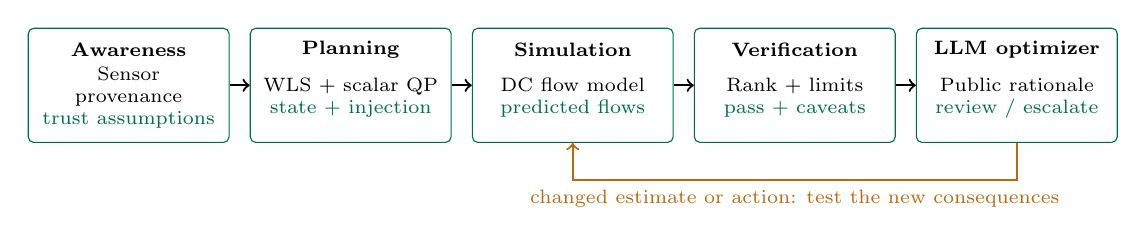
\begin{tikzpicture}[every node/.style={font=\scriptsize,align=center},b/.style={draw=forest,rounded corners=2pt,text width=2.34cm,minimum height=1.45cm,inner sep=3pt}]
\node[b] (a) at (0,0) {};
\node[font=\scriptsize\bfseries] at ([yshift=.45cm]a.center) {Awareness};
\uncover<1->{\node[text width=2.22cm] at ([yshift=-.16cm]a.center) {Sensor provenance\\\textcolor{forest}{trust assumptions}};}
\node[b] (p) at (2.82,0) {};
\node[font=\scriptsize\bfseries] at ([yshift=.45cm]p.center) {Planning};
\uncover<1->{\node[text width=2.22cm] at ([yshift=-.16cm]p.center) {WLS + scalar QP\\\textcolor{forest}{state + injection}};}
\node[b] (s) at (5.64,0) {};
\node[font=\scriptsize\bfseries] at ([yshift=.45cm]s.center) {Simulation};
\uncover<2->{\node[text width=2.22cm] at ([yshift=-.16cm]s.center) {DC flow model\\\textcolor{forest}{predicted flows}};}
\node[b] (v) at (8.46,0) {};
\node[font=\scriptsize\bfseries] at ([yshift=.45cm]v.center) {Verification};
\uncover<2->{\node[text width=2.22cm] at ([yshift=-.16cm]v.center) {Rank + limits\\\textcolor{forest}{pass + caveats}};}
\node[b] (o) at (11.28,0) {};
\node[font=\scriptsize\bfseries] at ([yshift=.45cm]o.center) {LLM optimizer};
\uncover<3->{\node[text width=2.22cm] at ([yshift=-.16cm]o.center) {Public rationale\\\textcolor{forest}{review / escalate}};}
\draw[->,thick] (a)--(p);\draw[->,thick] (p)--(s);\draw[->,thick] (s)--(v);\draw[->,thick] (v)--(o);
\uncover<3->{\draw[->,thick,orange] (o.south)--(11.28,-1.2)--node[below,font=\scriptsize]{changed estimate or action: test the new consequences}(5.64,-1.2)--(s.south);}
\end{tikzpicture}\end{center}
\textbf{Evidence provenance:} L8--L9 freshly evaluate the DC fixture; synthetic truth is for scoring, not given to the operating gate. L10 reads the separate archived five-stage Llama records.
\par\medskip
\uncover<4->{\textbf{Operator handoff:} retain the unverified trust assumptions. The recorded fixed and Llama routes use the same numerical control; improved attack detection is not established by the language layer.}

\slidetransition{Which failure boundary is common across the three cases?}
\sources{Actual recorded five-stage reference: \texttt{Proposal\_Complete\_Workflow.ipynb}, P1--P8; \texttt{results/proposal\_complete\_workflow.json}. Executed classroom experiment: \texttt{Classroom\_Labs.ipynb}; source: \texttt{src/classroom\_labs.py}. Teaching assumptions are explicit.}
\note{145--147 min. Point out that awareness and verification are substantial computational modules even when not every stage makes an LLM call. The stage table should be read as inputs and returned outputs. L10 later exposes all recorded responses and timings; it is not a fresh language-model run. Spoken bridge: Which failure boundary is common across the three cases?}
\end{frame}

\begin{frame}[t]{The three cases teach three different failure boundaries}

\begin{tabular}{@{}>{\raggedright\arraybackslash}p{.22\linewidth}>{\raggedright\arraybackslash}p{.34\linewidth}>{\raggedright\arraybackslash}p{.36\linewidth}@{}}
\toprule Case & What a naive workflow can miss & Evidence that addresses it \\
\midrule
Voltage & A reduced model omits a binding limit. & Broader-model validation and explicit scope. \\
Restoration & A good plan is applied after topology changes. & Fresh case-bound simulation and permissions. \\
Cyber & Plausible measurements describe the wrong state. & Justified trusted information or escalation. \\
\bottomrule
\end{tabular}\par
\par\medskip
\uncover<2->{\textbf{Common architecture:} choose tools, retain provenance, enforce contracts, expose limitations and involve the operator.}
\par\medskip
\uncover<3->{\textbf{Research question:} when does learning improve this architecture enough to justify its additional time, cost and failure modes?}

\slidetransition{How should we evaluate the next generation of this framework?}
\sources{Executed classroom experiment: \texttt{Classroom\_Labs.ipynb}; source: \texttt{src/classroom\_labs.py}. Teaching assumptions are explicit. Actual recorded voltage pilot: \texttt{LLM\_Response\_Selection.ipynb}, E1--E8; raw calls and numerical records in \texttt{results/ensemble\_voltage\_pilot/}. Schweppe \& Wildes, \href{https://doi.org/10.1109/TPAS.1970.292678}{state estimation (1970)}; Liu, Ning \& Reiter, \href{https://doi.org/10.1145/1653662.1653666}{false-data injection, CCS 2009}.}
\note{147--149 min. Give participants a minute to write one sentence for each case. Transition from case mechanics to current research and experimental evaluation. This is the common framework; it is not a claim that one numerical algorithm fits all tasks. Spoken bridge: How should we evaluate the next generation of this framework?}
\end{frame}

\section{Operator review}
% Four taught frames, approximately eight minutes. Sources refreshed 2026-10-17.
% Place after the three case debriefs and before the final operator discussion.

\begin{frame}[t]{Recent research asks when coordination is worth its cost}
\small\raggedright
\textbf{Research result:} Kim et al. study 260 configurations across six agent benchmarks. Collaboration depends on task structure and the capability of the single-agent baseline.
\medskip
\begin{tabular}{@{}>{\raggedright\arraybackslash}p{.27\linewidth}>{\raggedright\arraybackslash}p{.31\linewidth}>{\raggedright\arraybackslash}p{.34\linewidth}@{}}
\toprule Design choice & Possible benefit & What our experiment must measure \\
\midrule
Parallel specialists & Explore different candidates & Distinct valid actions per budget \\
Central coordinator & Preserve shared state and check handoffs & Stale evidence and rejected calls \\
Learned response selector & Allocate a trial using past feedback & Held-out reward and selection cost \\
\bottomrule
\end{tabular}\par
\medskip
\uncover<2->{\textbf{Return to L4 and E5.} The learned selector ties majority voting. A post-hoc fixed reactive-power rule produces the same actions. This result makes the added model calls a research question.}
\begin{alertblock}{Discussion, 30 seconds}
If three models propose the same action, what additional information has the ensemble supplied?
\end{alertblock}
\slidetransition{How can an effective procedure carry over to a new task?}
\sources{\href{https://arxiv.org/html/2512.08296v3}{Kim et al., agent-system scaling, v3 (2026)}. Published title: \href{https://doi.org/10.1038/s42256-026-01268-y}{Capable language models can outgrow the benefits of collaboration, Nature Machine Intelligence (2026)}. Tutorial evidence: E5, saved voltage pilot.}
\note{Allow two minutes. Bridge from the case results: now that the audience has seen actual candidates, they can assess architectural value. The six benchmarks in Kim et al. are general agent tasks, not grid operations. The architectural tradeoffs in this table are questions for our experiment, not reproduced findings. Ask learners to distinguish three model identities from three distinct physical actions. A candidate vote can convey agreement while adding no action diversity. The tutorial pays for the whole pool before selecting a trial, so it cannot claim the cost savings of routing a prompt to only one model. The voltage result is a null result about selector advantage, not proof that language interpretation never helps. Next: how can a useful procedure persist when the task or agent changes? Spoken bridge: How can an effective procedure carry over to a new task?}
\end{frame}

\begin{frame}[t]{Reusable skills make the procedure explicit}
\small\raggedright
\textbf{A recent power-system example.} Etingov and Biswas combine reusable skills, subagents and MCP-connected PSSE tools for power-flow and dynamic-study tasks.
\medskip
\begin{tabular}{@{}>{\raggedright\arraybackslash}p{.23\linewidth}>{\raggedright\arraybackslash}p{.69\linewidth}@{}}
\toprule A reusable procedure needs & Voltage-support example for this classroom \\
\midrule
Entry conditions & Current topology, trusted measurements and declared limits \\
Method and tools & MPC or SAC proposal, model execution and fresh verification \\
Evidence to return & Candidate ID, model scope, constraint margins and objective \\
Exit or escalation & Verified recommendation, or a reason to hold for review \\
\bottomrule
\end{tabular}\par
\medskip
\uncover<2->{\textbf{Code connection, L1.} \texttt{bind\_evidence} ties the result to its request and candidate. \texttt{bound\_to} rejects a changed load or command.}
\begin{block}{A small experiment}
Remove the model scope from a handoff. Decide which later claim can no longer be justified.
\end{block}
\slidetransition{Which decisions require an enforced authority boundary?}
\sources{\href{https://arxiv.org/abs/2609.40272v2}{Etingov and Biswas, Skill-Based AI Agents for Power-System Studies, v2 (1 October 2026), preprint}. Context design: \href{https://www.anthropic.com/engineering/effective-context-engineering-for-ai-agents}{Anthropic, Effective context engineering (2025), engineering guidance}. Table: proposed classroom procedure.}
\note{Allow two minutes. A skill packages a procedure, while a tool performs a specific operation. The cited recent study uses PSSE and distinct agent implementations. Our tutorial uses Python tools and does not reproduce its platform or performance. The purpose of this slide is to make the existing numerical workflow reusable without losing assumptions. A language summary may compress details that the state contract must retain exactly. Ask the audience what an OpenDSS verification establishes if the prior record only says PASS. Answer: without model scope and identity they cannot determine which candidate or part of the network passed. The exercise is a review of the existing handoff, not a live mutation of the scientific archive. Next: preserved evidence still needs a defined authority boundary. Spoken bridge: Which decisions require an enforced authority boundary?}
\end{frame}

\begin{frame}[t]{Control-room authority belongs in executable rules}
\small\raggedright
\textbf{2026 governance study:} an external layer enforces tool permissions, step budgets, operator approval and numerical provenance. Its prototype reports 93.7\% task success and 100\% rule compliance in 590 runs.
\medskip
\begin{center}
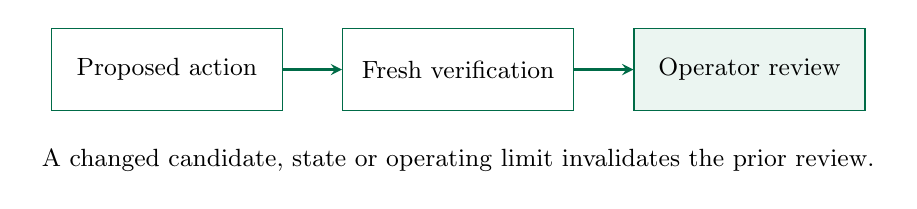
\begin{tikzpicture}[x=1cm,y=1cm,
  state/.style={draw=forest,fill=white,text width=2.7cm,minimum height=1.05cm,align=center,font=\small},
  flow/.style={->,>=stealth,thick,forest}]
\node[state] (p) at (0,0) {Proposed action};
\node[state] (v) at (3.7,0) {Fresh verification};
\node[state,fill=mint!25] (h) at (7.4,0) {Operator review};
\uncover<2->{\draw[flow] (p)--(v);}
\uncover<3->{\draw[flow] (v)--(h);}
\node[align=center,font=\small,text width=10.7cm] at (3.7,-1.15) {A changed candidate, state or operating limit invalidates the prior review.};
\end{tikzpicture}
\end{center}
\begin{tabular}{@{}>{\raggedright\arraybackslash}p{.47\linewidth}>{\raggedright\arraybackslash}p{.47\linewidth}@{}}
\textbf{The rule can hold} & \textbf{The task can still fail} \\
An approval gate blocks unapproved actions. & The proposal may name the wrong equipment. \\
A number points to a backend result. & The agent may choose the wrong source. \\
\end{tabular}\par
\medskip
\textbf{Lab L12:} \texttt{operator\_packet} checks the required scope. \texttt{acknowledge} checks readback identity. The endpoint remains advisory.
\slidetransition{How could we test the benefit of this orchestration fairly?}
\sources{\href{https://arxiv.org/html/2609.22476v1}{Mylonas, Foti and Varvarigos, Governance-Aware Agentic Digital Twin for TSO Control Rooms (18 September 2026), preprint, \S6}. Diagram: tutorial review boundary.}
\note{Allow two minutes. Point to the separation between language capability and runtime enforcement. The cited paper's rule compliance concerns its tested prototype and trusted governance layer. Its authors explicitly reserve measurement of operator benefit for a subsequent study. In our classroom, state and candidate identity allow a reviewer to see exactly what has been checked. A wrong-source result can be perfectly traceable, so provenance and correctness require separate evaluation. Ask learners which acknowledgment should remain valid after changing the voltage threshold: none of the earlier approvals should authorize the changed recommendation. Keep the endpoint advisory. This is the reason the operator screen presents limits, model scope and rejected alternatives alongside the concise Llama explanation. Spoken bridge: How could we test the benefit of this orchestration fairly?}
\end{frame}

\begin{frame}[t]{The next study should isolate workflow value}
\small\raggedright
\textbf{A testable question:} does agentic orchestration complete unfamiliar operator requests more reliably with the same engineering tools and budget?
\medskip
\begin{tabular}{@{}>{\raggedright\arraybackslash}p{.22\linewidth}>{\raggedright\arraybackslash}p{.34\linewidth}>{\raggedright\arraybackslash}p{.36\linewidth}@{}}
\toprule Comparison & Hold fixed & Measure separately \\
\midrule
Scripted workflow vs. Llama orchestration & Models, observations, limits and available tools & Correct intent, completed stages and unsupported claims \\
One LLM vs. several roles & Base model and total tool/token budget & Handoff errors, recovery and latency \\
Fixed vs. vote vs. learned selection & Response pool, trial budget and frozen test set & Feasibility, objective and selection overhead \\
\bottomrule
\end{tabular}\par
\medskip
\uncover<2->{\textbf{Stress extension:} change forecast uncertainty or the model scope, then repeat the audit. Keep test outcomes out of prompts and learned-selector updates.}
\begin{alertblock}{Exit question}
Which measured outcome would justify adding one more agent to your control-room workflow?
\end{alertblock}
\slidetransition{What time did the extra coordination actually cost?}
\sources{Evidence-based scoring: \href{https://arxiv.org/html/2606.18789v1}{PowerAgentBench-SS (June 2026)}. Uncertainty-aware orchestration: \href{https://arxiv.org/html/2606.24609v1}{CONDUCTOR (June 2026)}. Table: proposed evaluation design, not a reported experiment.}
\note{Allow two minutes. This slide closes the research section with a concrete experimental design. Accept multiple well-defined answers to the exit question, such as fewer incorrect interpretations at equal electrical feasibility and acceptable latency, or fewer unsupported readiness claims under model mismatch. Numerical objective improvement is another possible outcome, but it must be demonstrated rather than assumed. A matched scripted baseline can use the same verifier and numerical solvers. More validation calls must be accounted for. CONDUCTOR motivates a richer analysis surface; our forecast perturbations would be a classroom sensitivity experiment, not a reproduction or a calibrated operational risk estimate. PowerAgentBench-SS motivates separate evidence and physical scores. Operator workload needs an actual human study. Transition to the final operator review: the audience now has a criterion for judging whether to trust, reject or extend the workflow. Spoken bridge: What time did the extra coordination actually cost?}
\end{frame}

\begin{frame}[t]{Latency must be measured where the work actually happens}

\begin{center}\includegraphics[width=.97\linewidth,height=.47\textheight,keepaspectratio]{\figfile{selector_E7.png}}\end{center}
\small
\textbf{Recorded experiment:} 168 real local-model calls. MV mean accounted serial time: learned selection 8.119 s; fixed numerical refinement 3.327 s.
\par\medskip\par
\uncover<2->{\textbf{Separate:} solver time, LLM load/inference, retries and final verification. Cached notebook display time is not inference latency. The AC transfer reused MPC planning and reports that component separately.}

\slidetransition{What can we inspect in one real local Llama call?}
\sources{Actual recorded voltage pilot: \texttt{LLM\_Response\_Selection.ipynb}, E1--E8; raw calls and numerical records in \texttt{results/ensemble\_voltage\_pilot/}.}
\note{157--159 min. Research frontier has occupied 149--157. Read the latency axis and distinguish actual raw call times from a sum of components. Parallel service would have different wall-clock behavior and cannot be inferred from these serial accounts. No latency confidence interval establishes production deadline compliance. Spoken bridge: What can we inspect in one real local Llama call?}
\end{frame}

\begin{frame}[t]{Lab 11: one optional local Llama call, with visible provenance}

\checkpoint{L11}{Default is offline; explicitly enable the optional local call.}
\cellcode{L11}{6}{8}
\small
\textbf{Actual validation, 17 October 2026:} Llama 3.1 8B chose \texttt{RELAX\_Q\_10\_PERCENT} on the original test\_01 context.
\uncover<2->{\begin{block}{Excerpt from the returned public reason}
\small ``the RELAX\_Q\_10\_PERCENT operation has the potential to reduce reactive effort magnitude by ten percent, which may improve the cost.''
\end{block}}
\uncover<3->{\textbf{Observed time:} 34.113 s client elapsed; Ollama reported 16.967 s loading, 15.192 s prompt processing and 1.916 s generation.}
\par\medskip
This is one call, shown from its saved record. The default L11 makes no new call. Inspect the complete response and mode in the notebook; a reason still requests a fresh trial.

\slidetransition{Which outcomes must we score separately?}
\sources{\href{https://docs.ollama.com/api/chat}{Ollama chat API}; \href{https://arxiv.org/abs/2407.21783}{Llama 3 model report (2024)}; actual record: \texttt{results/classroom\_optional\_llama\_validation.json}; Executed classroom experiment: \texttt{Classroom\_Labs.ipynb}; source: \texttt{src/classroom\_labs.py}. Teaching assumptions are explicit.}
\note{159--161 min. Optional instructor live demo only; do not let model download consume class time. The audience can use saved real responses. Show the process boundary: this requests language output from a local runtime, not equipment dispatch. Warm/cold loading and hardware affect measured latency. Explain any invalid JSON or failure transparently. Spoken bridge: Which outcomes must we score separately?}
\end{frame}

\begin{frame}[t]{Evaluate the failure, the recovery and the final outcome separately}

\begin{tabular}{@{}>{\raggedright\arraybackslash}p{.23\linewidth}>{\raggedright\arraybackslash}p{.32\linewidth}>{\raggedright\arraybackslash}p{.37\linewidth}@{}}
\toprule Metric & Question & Common mistaken conclusion \\
\midrule
Task completion & Did the intended study finish? & Valid JSON means success. \\
Electrical feasibility & Which constraints passed, on which model? & Solver convergence means safe. \\
Recovery & Was the failed attempt repaired within budget? & More retries mean intelligence. \\
Claim support & Does each numerical statement match evidence? & A fluent reason is evidence. \\
Operator benefit & Did correct decisions improve with acceptable workload? & A dashboard proves human benefit. \\
\bottomrule
\end{tabular}\par
\par\medskip
\textbf{Our evidence supports an executable teaching workflow.} A field claim would need broader scenarios, stronger models and a study with operators.

\slidetransition{What evidence should reach the operator?}
\sources{\href{https://arxiv.org/abs/2604.10846}{PFAgent (2026)}; \href{https://arxiv.org/abs/2606.18789}{PowerAgentBench-SS (2026)}; \href{https://arxiv.org/abs/2503.13657}{MAST failure taxonomy}.}
\note{161--162 min. One-minute synthesis of evaluation. These dimensions should be recorded independently. A rejected trial may be evidence the guard worked, yet still consume time. A low false-alarm rate can coexist with missed stealth attacks. Move to the operator capstone. Spoken bridge: What evidence should reach the operator?}
\end{frame}



\begin{frame}[t]{The control room receives a recommendation with an evidence trail}

\begin{columns}[T]
\column{.51\textwidth}
\includegraphics[width=\linewidth,height=.56\textheight,keepaspectratio]{\figfile{proposal_control_room.png}}
\scriptsize Concept illustration; AI-generated, not a deployed control room.
\column{.46\textwidth}
\textbf{What the operator needs}\par
Requested action and exact equipment or candidate ID.\par\medskip
Current case, model scope and constraint margins.\par\medskip
Failed alternatives, unresolved assumptions and age of evidence.\par\medskip
Concise public rationale, with each numerical claim tied to a tool result.
\end{columns}
\par\smallskip\small Deployment concept: advisory service beside existing operational applications; authorized procedures govern any later field action.

\slidetransition{How does a review become an explicit acknowledgment?}
\sources{\href{https://arxiv.org/abs/2609.22476}{Governance-aware TSO digital twin (2026)}; illustration provenance in \texttt{figures/Proposal\_Illustration\_Provenance.md}.}
\note{162--164 min. Explain the deployment boundary: notebook, numerical sandbox and advisory review are implemented; operational integration is a concept. Do not suggest the synthetic feeder is a live network. Ask what the operator would need to see before reviewing a change during a busy shift. Spoken bridge: How does a review become an explicit acknowledgment?}
\end{frame}

\begin{frame}[t]{Lab 12: acknowledgment is a state transition, not a generated sentence}

\checkpoint{L12}{Build an operator packet and test the readback gate.}
\cellcode{L12}{9}{10}
\exercise{4}{Try a wrong candidate ID, then the correct readback. Change the requested control after review. Decide whether the old acknowledgment should remain valid.}
\begin{center}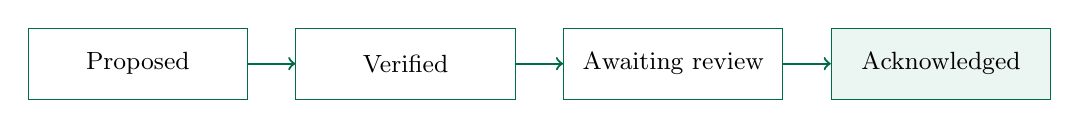
\begin{tikzpicture}[every node/.style={font=\small,align=center},b/.style={draw=forest,text width=2.55cm,minimum height=.9cm}]
\node[b] (a) at (0,0) {Proposed};\node[b] (b) at (3.4,0) {Verified};\node[b] (c) at (6.8,0) {Awaiting review};\node[b,fill=mint!25] (d) at (10.2,0) {Acknowledged};
\uncover<2->{\draw[->,thick,forest] (a)--(b);}\uncover<3->{\draw[->,thick,forest] (b)--(c);}\uncover<4->{\draw[->,thick,forest] (c)--(d);}
\end{tikzpicture}\end{center}
\small This is a local advisory exercise. No state in this notebook dispatches equipment.

\slidetransition{Can we reconstruct every stage from one saved trace?}
\sources{Executed classroom experiment: \texttt{Classroom\_Labs.ipynb}; source: \texttt{src/classroom\_labs.py}. Teaching assumptions are explicit. Runtime authority: \href{https://arxiv.org/abs/2609.22476}{Mylonas et al. (2026)}.}
\note{164--168 min. Four minutes hands-on. The operator reviews a specific packet; a language model cannot acknowledge on their behalf. Wrong identity is rejected. If a changed action is not reverified, a prior approval cannot carry over. A completed readback is still not proof the operator understood the evidence; that needs human-factors evaluation. Spoken bridge: Can we reconstruct every stage from one saved trace?}
\end{frame}

\begin{frame}[t]{One trace should answer what happened at every stage}

\checkpoint{L10}{Compare real saved stage records and public responses.}
\cellcode{L10}{1}{3}\footnotesize
\begin{tabular}{@{}>{\raggedright\arraybackslash}p{.22\linewidth}>{\raggedright\arraybackslash}p{.69\linewidth}@{}}
\toprule Inspect & What the answer should expose \\
\midrule
Input & Case, measurement assumptions, allowed operations and model scope. \\
Method & Which optimizer, policy, simulator or language call actually ran. \\
Output & Candidate ID, returned values, constraint failures and public reason. \\
Cost & Measured tool/call time, including failed attempts. \\
Disposition & Retained, rejected, refined or escalated; the next required step. \\
\bottomrule
\end{tabular}\par
\par\medskip
\textbf{Trace labels matter:} classroom fresh solve, archived actual LLM response and optional live call are different evidence modes.

\slidetransition{Which missing evidence changes the operator decision?}
\sources{Executed classroom experiment: \texttt{Classroom\_Labs.ipynb}; source: \texttt{src/classroom\_labs.py}. Teaching assumptions are explicit. Actual recorded five-stage reference: \texttt{Proposal\_Complete\_Workflow.ipynb}, P1--P8; \texttt{results/proposal\_complete\_workflow.json}.}
\note{168--170 min. L10 is archived five-stage evidence, clearly labeled. The fresh classroom methods are related but are not retroactively given those old language responses. Ask students to find a stage that uses a deterministic method and explain why it still belongs in the agentic workflow. Each role has a responsibility, not necessarily its own model process. Spoken bridge: Which missing evidence changes the operator decision?}
\end{frame}

\begin{frame}[t]{Capstone: would you approve, hold or request another study?}

\begin{tabular}{@{}>{\raggedright\arraybackslash}p{.13\linewidth}>{\raggedright\arraybackslash}p{.57\linewidth}>{\raggedright\arraybackslash}p{.22\linewidth}@{}}
\toprule Card & Evidence presented & Your decision \\
\midrule
A & MV PASS; full-feeder AC FAIL; Llama says ``ready''. & Review / hold / study? \\
B & Restoration MILP PASS; equipment isolation has no supporting record. & Review / hold / study? \\
C & No residual alarm; protected measurement set is unavailable. & Review / hold / study? \\
\bottomrule
\end{tabular}\par
\par\medskip
\textbf{Task:} identify the missing fact and the appropriate tool or human step. Do not answer with a model's confidence score.
\uncover<2->{\par\medskip\textbf{Debrief:} A requires broader-model repair; B requires authorized isolation evidence; C requires justified independent information or escalation. None supports automatic dispatch.}

\slidetransition{Which architecture fits each kind of operator task?}
\sources{Executed classroom experiment: \texttt{Classroom\_Labs.ipynb}; source: \texttt{src/classroom\_labs.py}. Teaching assumptions are explicit. Schweppe \& Wildes, \href{https://doi.org/10.1109/TPAS.1970.292678}{state estimation (1970)}; Liu, Ning \& Reiter, \href{https://doi.org/10.1145/1653662.1653666}{false-data injection, CCS 2009}.}
\note{170--172 min. Ask one row per group. These cards are intentionally distinct: model scope, physical permission and information trust. The correct answer includes a concrete next action rather than simply no. Do not imply that holding a prior setting is always safe after a topology or measurement change. Spoken bridge: Which architecture fits each kind of operator task?}
\end{frame}

\begin{frame}[t]{Match the architecture to the operator task}

\begin{tabular}{@{}>{\raggedright\arraybackslash}p{.30\linewidth}>{\raggedright\arraybackslash}p{.31\linewidth}>{\raggedright\arraybackslash}p{.31\linewidth}@{}}
\toprule Task condition & Useful architecture & Evidence required \\
\midrule
Stable repeated calculation & Fixed workflow + numerical checks & Correct model and tested contract. \\
Varied language requests & LLM tool selection + typed state & Intent accuracy and supported claims. \\
Several independent studies & Bounded specialist roles & Handoff quality and real parallel benefit. \\
Competing refinements & Vote or learned selector & Held-out gain at equal trial budget. \\
High-consequence action & Human review + enforced authorization & Correct action, scope, provenance and permissions. \\
\bottomrule
\end{tabular}\par
\par\medskip
\textbf{Design principle:} add complexity only when it solves a measured failure of the simpler workflow.

\slidetransition{Can you explain one complete case using the five stages?}
\sources{\href{https://arxiv.org/abs/2512.08296v3}{Kim et al., scaling agent systems (2026)}; \href{https://arxiv.org/abs/2609.22476}{governance-aware TSO study (2026)}.}
\note{172--174 min. This table is a synthesis, not a ranking of packages. Ask learners to choose the simplest design for their own use case. A deterministic workflow can include the same engineering verifier and operator controls; those features are not exclusive benefits of an LLM. Spoken bridge: Can you explain one complete case using the five stages?}
\end{frame}


\begin{frame}[t]{Explain the full workflow in sixty seconds}

\textbf{Awareness:} establish the current case and what is known.\par\medskip
\textbf{Planning:} choose an appropriate numerical method and form candidates.\par\medskip
\textbf{Simulation:} calculate each candidate's consequences in a declared model.\par\medskip
\textbf{Verification:} check physical limits, identity, evidence and permissions.\par\medskip
\textbf{LLM optimizer:} propose a bounded next trial, then return through simulation and verification.\par\medskip
\textbf{Operator review:} inspect the recommendation and unresolved assumptions before any authorized action.
\par\medskip
\textcolor{forest}{\textbf{Partner exercise:}} use one of today's cases and name the actual method and output at every stage.

\slidetransition{Which comparisons support a scientific claim?}
\sources{Executed classroom experiment: \texttt{Classroom\_Labs.ipynb}; source: \texttt{src/classroom\_labs.py}. Teaching assumptions are explicit.}
\note{174--176 min. Give one minute per pair, then ask for a concise example. Do not accept merely reciting agent names; require MPC, SAC, MILP, WLS, QP or a numerical model where appropriate. The physical simulation stage does not execute field actions. Spoken bridge: Which comparisons support a scientific claim?}
\end{frame}

\begin{frame}[t]{Three checks for scientific claims about agentic control}

\textbf{1. Is the comparison matched?}\par
Same observations, model coverage, limits, tools, candidate budget and test scenarios?\par\medskip
\textbf{2. Which component caused the difference?}\par
Better optimizer, broader model, protected information, language interpretation or coordination?\par\medskip
\textbf{3. What was actually measured?}\par
Constraint compliance, objective, task completion, claim support, latency or human performance?\par\medskip
\uncover<2->{\textbf{Today's result:} the framework makes these questions executable. Extra language models and learned selection did not establish general superiority in the recorded pilot.}

\slidetransition{What single assumption would you change in the next experiment?}
\sources{\href{https://arxiv.org/abs/2606.18789}{PowerAgentBench-SS (2026)}; Actual recorded voltage pilot: \texttt{LLM\_Response\_Selection.ipynb}, E1--E8; raw calls and numerical records in \texttt{results/ensemble\_voltage\_pilot/}.}
\note{176--178 min. This is the scientific takeaway, not a marketing conclusion. Participants should be able to reject an unfair DRL-versus-agentic comparison where the latter receives a better model or more trials. Ask which ablation they would run next. Spoken bridge: What single assumption would you change in the next experiment?}
\end{frame}

\begin{frame}[t]{Your next experiment: change one assumption and keep an audit trail}

\begin{tabular}{@{}>{\raggedright\arraybackslash}p{.20\linewidth}>{\raggedright\arraybackslash}p{.43\linewidth}>{\raggedright\arraybackslash}p{.29\linewidth}@{}}
\toprule Extension & Change one thing & Keep fixed \\
\midrule
Voltage & Forecast uncertainty or a current margin & Controls, model scope and trial budget. \\
Restoration & Priority weights or one tie rating & Fault, graph and baseline constraints. \\
Cyber & Sensor trust or noise assumptions & Physical truth and scoring protocol. \\
Agent design & One role, prompt or selector feature & Tools, test split and numerical gates. \\
\bottomrule
\end{tabular}\par
\par\medskip
\textbf{Deliverable:} one plot, a baseline comparison, a trace explaining the result and a statement of what remains unproven.
\par\medskip
\textbf{After class:} the appendix contains derivations, full code excerpts, recorded responses and training details. It is reference material outside the 180-minute route.

\slidetransition{Choose an extension, then use the appendix when you need its derivation.}
\sources{Executed classroom experiment: \texttt{Classroom\_Labs.ipynb}; source: \texttt{src/classroom\_labs.py}. Teaching assumptions are explicit. Reading guide: \texttt{appendix/Agentic\_AI\_Research\_2026.md}.}
\note{178--180 min. End with an achievable research task, not additional lecture content. Invite participants to choose one extension and write a hypothesis. The teaching session ends here; the appendix is not part of the time budget. Answer final questions and point to the source package and classroom notebook. Spoken bridge: Choose an extension, then use the appendix when you need its derivation.}
\end{frame}


\ifdefined\LectureOnly\else
\appendix
\def\InClassroomAppendix{1}
\section{Technical appendix}
\begin{frame}{Technical appendix: use after the three-hour class}
\small
The taught sequence ends at frame \LectureFrameCount. The following pages preserve deeper derivations, implementation excerpts, recorded studies and full mathematical definitions.\par\medskip
\textbf{G0--G5:} real LangGraph teaching example, with declared toy current.\par\smallskip
\textbf{L0--L12:} current classroom notebook, used in the lecture.\par\medskip
\textbf{S/W/M/V/A/R/C/F:} original numerical workshop.\par\medskip
\textbf{P:} archived five-stage workflow; \textbf{E:} archived response-selector pilot; \textbf{T:} archived latency analysis.\par\medskip
These are separate experiments. Their numerical results, model scopes and call timings must not be mixed into a single experiment.
\slidetransition{Which physical limit couples active and reactive power?}
\sources{Exact mapping and source hashes: \texttt{Slide\_Notebook\_Map.md} and \texttt{checkpoints.json}.}
\note{Outside the 180-minute route. Choose individual appendix pages in response to questions or for an advanced follow-up session. The source package retains all original section files, including material not selected into this appendix.}
\end{frame}
\begin{frame}[t]{Two controls share one inverter capability}
\small\setlength{\parskip}{0.1em}
\ask{At active participation $p/S=1$, can the inverter also supply reactive power?}
\begin{columns}[c,onlytextwidth]
\begin{column}{0.49\linewidth}
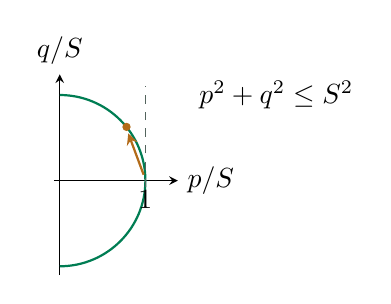
\begin{tikzpicture}[scale=0.75,>=stealth]
\draw[->] (-0.1,0)--(2.0,0) node[right]{$p/S$};
\draw[->] (0,-1.6)--(0,1.8) node[above]{$q/S$};
\draw[teal,thick] (0,-1.45) arc[start angle=-90,end angle=90,radius=1.45];
\draw[slate,dashed] (1.45,-.1)--(1.45,1.6);
\node[below] at (1.45,0){1};
\node[right] at (2.2,1.45){$p^2+q^2\leq S^2$};
\uncover<2->{\fill[orange] (1.13,.91) circle(2pt);
\draw[orange,->,thick] (1.42,.1)--(1.16,.8);}
\end{tikzpicture}
\end{column}
\begin{column}{0.47\linewidth}
\textbf{Active power $p$ (kW):} delivered PV production; nonnegative here.

\medskip
\textbf{Reactive power $q$ (kvar):} injection if positive, absorption if negative. Both affect voltage and current.

\medskip
$S$ (kVA) is the inverter rating; $p/S$ and $q/S$ are dimensionless. The circle is a device limit, not a network-feasibility test.
\end{column}
\end{columns}
\answer{No. More reactive support can require less active output. We must check the resulting network currents as well as voltage.}
\slidetransition{Which limits turn the request into an optimization problem?}
\sources{Implemented device domain: \texttt{src/standard\_formulations.py}; physical model: \href{https://opendss.epri.com/PowerFlow.html}{EPRI OpenDSS}. Diagram illustrates capability, not a measured point.}
\note{Optional historical/detail reference, outside the current 180-minute route. Original notebook IDs and experiment scopes are preserved. 37--39 minutes. Ask for a prediction before advancing the overlay. The drawing shows the positive-active-power half of the normalized capability circle, with equal axis scales. Positive generator q means injection and negative q absorption. Neither sign universally improves every constraint. The orange point illustrates a tradeoff, not a measured operating point. Bridge: convert these engineering limits and preferences into an optimization problem. Spoken bridge: Which limits turn the request into an optimization problem?}
\end{frame}

\begin{frame}[t]{Turn the operating request into a checkable problem}
\small
\textbf{General Volt/VAR OPF:} choose active/reactive setpoints $p,q$ to minimize
\[
 C_{\rm PV}(p)+C_v(v)+C_q(q),\qquad
 v_{\min}\leq v_{i\phi}\leq v_{\max},\quad
 |I_{\ell\phi}|\leq\rho I^{\rm rated}_{\ell\phi},\quad
 p_g^2+q_g^2\leq S_g^2 .
\]
The selected three-phase power-flow equations also hold; $0\leq p_g\leq p_g^{\rm av}$ and device reactive bounds apply.
\footnotesize
\begin{tabular}{@{}p{.24\linewidth}p{.68\linewidth}@{}}
\toprule Symbol & Definition and physical interpretation \\
\midrule
$i,\phi,\ell,g$ & Bus, available phase, line/conductor, and inverter indices. \\
$v_{i\phi}$, $v_{\min},v_{\max}$ & Voltage magnitude and allowed bounds (p.u.); here $0.95$ and $1.05$. \\
$I_{\ell\phi}$, $I^{\rm rated}_{\ell\phi}$ & Predicted current magnitude and nominal rating (A). $\rho\in(0,1]$ is the permitted rating fraction. \\
$p_g,q_g,S_g,p_g^{\rm av}$ & Active output (kW), reactive output (kvar), rating (kVA), and available PV (kW). \\
$C_{\rm PV},C_v,C_q$ & Weighted penalties for curtailment, voltage deviation and reactive effort; weights reconcile units and state the preference. \\
\bottomrule
\end{tabular}
\smallskip\par\small\textbf{Agent boundary:} preserve the objective, limits and permissions; numerical tools compute and check the setpoints.
\slidetransition{Which quantities can this particular experiment control?}
\sources{General three-phase formulation: Gan and Low (2014), \url{https://arxiv.org/abs/1406.3054}. Full objective, units and constraints are in the mathematical appendix.}
\note{Optional historical/detail reference, outside the current 180-minute route. Original notebook IDs and experiment scopes are preserved. 39--41 minutes. C\_PV penalizes curtailed PV power; C\_v penalizes voltage deviation from a declared target; C\_q can penalize reactive effort. Explain each symbol next to its use. Phi labels a phase, i a bus, ell a branch and g an inverter. Available PV and per-device reactive limits also constrain the problem and remain in the implementation. Ask whether a very good objective permits violating current: no. Bridge: the general formulation may have many device variables; we use a transparent two-variable reduction for this experiment. Spoken bridge: Which quantities can this particular experiment control?}
\end{frame}

\begin{frame}[t]{What does this teaching experiment actually control?}
\small
All 930 inverters share \textbf{two dimensionless controls}; this is a reduced continuous OPF:
\[
p_g=aS_g,\quad q_g=bS_g,\qquad
0\leq a\leq1,\quad |b|\leq0.44,\quad a^2+b^2\leq1.
\]
Here $g$ identifies an inverter, $S_g$ is its kVA rating, $p_g$ is kW, and $q_g$ is kvar. The high-irradiance overlay assumes available active power equals rated kVA.
\[
C(a,b)=\underbrace{(1-a)^2}_{\text{PV curtailment}}+
\underbrace{0.05b^2}_{\text{reactive effort}}+
\underbrace{\frac{10}{N_v}\sum_{j=1}^{N_v}(v_j-1.01)^2}_{\text{voltage regulation}}.
\]
\footnotesize $C$ is a dimensionless teaching cost, not money; its coefficients are declared preferences. $v_j$ is the $j$th modeled energized node-phase voltage in p.u.; $N_v$ counts those samples; $1.01$ p.u. is the target.
\smallskip\par\small
\textbf{How it is solved:} finite differences form local sensitivities; bounded QP steps use an inscribed 32-sided capability polygon. A fresh backend solve checks each candidate. A feasible local improvement is not a global AC optimum.
\slidetransition{What operating point does the numerical optimizer return?}
\sources{Teaching implementation: \texttt{src/standard\_formulations.py}; general phase-coupled formulation: \href{https://arxiv.org/abs/1406.3054}{Gan and Low (2014)}.}
\note{Optional historical/detail reference, outside the current 180-minute route. Original notebook IDs and experiment scopes are preserved. 41--43 minutes. Walk through the three underbraces: normalized curtailment, reactive effort and mean squared voltage deviation. The coefficients are teaching preferences rather than calibrated economic prices. All 930 devices share the two factors; this is not independent per-inverter optimal control. The declared high-irradiance overlay makes available active power equal to rated kVA. Device kvar bounds and an inner capability polygon are enforced. The algorithm is a sequence of local QPs, not a global nonlinear optimality proof. Bridge: run it and inspect the returned control and fresh check. Spoken bridge: What operating point does the numerical optimizer return?}
\end{frame}

\begin{frame}[t]{V1: ask the optimizer for a better operating point}
\checkpoint{V1}{Run the complete cell; this line performs the optimization.}
\cellcode{V1}{1}{1}
\small
\begin{tabular}{@{}lrrrr@{}}
\toprule Selected MV model & Total $p$ (MW) & Total $q$ (MVAr) & $v_{\max}$ (p.u.) & Current (\%)\\
\midrule
Before & 7.850 & 0.000 & 1.0480 & 60.8\\
After & 7.727 & -1.249 & 1.0370 & 65.3\\
\bottomrule
\end{tabular}
\par\smallskip\footnotesize Current = maximum line/conductor current as a percentage of nominal rating; $v_{\max}$ is the largest modeled voltage magnitude.\par\normalsize
\observethis{The objective falls from $0.00760$ to $0.00549$. Both points pass the MV check; the optimized point trades some active power and reactive effort for voltage regulation.}
\slidetransition{Which constraint can become worse when voltage improves?}
\sources{Recorded LinDistFlow result: \texttt{results/standard\_formulations.json}; code checkpoint V1. Model: \href{https://arxiv.org/abs/1406.3054}{Gan and Low (2014)}.}
\note{Optional historical/detail reference, outside the current 180-minute route. Original notebook IDs and experiment scopes are preserved. 43--46 minutes. Give participants time to run V1 and find the same quantities in its returned table. These figures are from the executed selected LinDistFlow route. Negative q means absorption. Do not infer a safety improvement from an infeasible baseline: both baseline and optimized points are feasible in this model. The optimizer's accepted flag includes a fresh backend solve and dispatch-tracking checks. Ask how much P was reduced and whether current moved in the expected direction. Bridge: extrema summarize a point, but a plot makes the simultaneous changes easier to see. Spoken bridge: Which constraint can become worse when voltage improves?}
\end{frame}

\begin{frame}[t]{V2: better voltage can come with higher current}
\checkpoint{V2}{Run the plot and compare the two curves in each panel.}
\begin{center}
\includegraphics[width=.95\linewidth,height=.43\textheight,keepaspectratio]{\figfile{workshop_voltage_lindistflow3.png}}
\end{center}
\observethis{Voltage moves toward the target; current increases. Both remain within the \textbf{modeled} limits.}
\slidetransition{What changes if only reactive power can move?}
\sources{Actual snapshot plot: \texttt{results/workshop\_run\_lindistflow3.json}, checkpoint V2. Model: \href{https://arxiv.org/abs/1406.3054}{Gan and Low (2014)}.}
\note{Optional historical/detail reference, outside the current 180-minute route. Original notebook IDs and experiment scopes are preserved. 46--48 minutes. Ask participants to identify the baseline and optimized curve before explaining. Horizontal positions are sorted samples, not geographic bus positions. The limit lines use the selected MV model's normal ratings. The plot demonstrates a tradeoff, not a universal sign rule for reactive power. Bridge: hold active power fixed and predict the effect of changing only reactive power. Spoken bridge: What changes if only reactive power can move?}
\end{frame}

\begin{frame}[t]{Hold active power fixed; change only reactive power}
\exercise{3}{Predict first: how will absorption affect voltage and current at the same active output?}
\begin{enumerate}
\item Create a scratch \texttt{PQBackend(BACKEND)} for the selected model.
\item Solve $u_1=(0.8,0)$, then $u_2=(0.8,-0.1)$ using that scratch model.
\item Compare achieved P/Q, maximum voltage and current; keep V1's result unchanged.
\end{enumerate}
\small The dimensionless vector $u=(a,b)$ sets active and reactive participation; $u_1,u_2$ label the two trials. Explain the observed tradeoff in one sentence. A point with lower voltage can still have higher current.
\slidetransition{Will the same control pass the fuller model?}
\sources{Exercise uses \texttt{src/standard\_formulations.py}; models: \href{https://opendss.epri.com/PowerFlow.html}{EPRI OpenDSS} / \href{https://arxiv.org/abs/1406.3054}{Gan and Low (2014)}.}
\note{Optional historical/detail reference, outside the current 180-minute route. Original notebook IDs and experiment scopes are preserved. 48--51 minutes. Compare two exact points in a scratch PQBackend without changing stored V1 or V2 output. Both settings satisfy the fleet capability circle. Calling the same scratch model twice permits a controlled P/Q comparison. Do not pass a new load multiplier to the older snapshot LinDistFlow adapter, which intentionally rejects that argument. A prediction need not be right; report what the selected backend returns. Bridge: would the same control pass a wider model boundary? Spoken bridge: Will the same control pass the fuller model?}
\end{frame}

\begin{frame}[t]{V3: does the same control pass a fuller audit?}
\checkpoint{V3}{Read the recorded comparison; do not change the control between checks.}
\ask{Does an MV-only pass establish an acceptable full-feeder AC result?}
The same aggregate PV outputs are $p=7.727$ MW and $q=-1.249$ MVAr; negative $q$ means absorption.
\small
\begin{tabular}{@{}lrrl@{}}
\toprule Evaluation of that point & Max. voltage (p.u.) & Nominal current (\%) & Result\\
\midrule
MV-only LinDistFlow & 1.037 & 65.3 & Pass\\
\uncover<2->{Full-feeder OpenDSS audit} & \uncover<2->{1.087} & \uncover<2->{288.2} & \uncover<2->{Fail}\\
\bottomrule
\end{tabular}
\normalsize
\answer{No. The MV model omits LV constraints. The full OpenDSS optimizer finds a different checked point: $2.904$ MW and $0.346$ MVAr.}
\slidetransition{How does a horizon plan extend a single operating point?}
\sources{Identical-control audit and separate optimized AC point: \texttt{results/standard\_formulations.json}; \href{https://opendss.epri.com/PowerFlow.html}{EPRI OpenDSS}.}
\note{Optional historical/detail reference, outside the current 180-minute route. Original notebook IDs and experiment scopes are preserved. 51--53 minutes. Let participants predict before advancing. The audit evaluates identical controls; its failure is not a secret repair. The separate OpenDSS optimized point has maximum voltage 1.043224 pu and current 99.8913 percent, with zero checked violations. These are recorded comparisons, not a claim that V1 ran both backends. Explain why larger permitted PV in an MV-only model is not automatically a superior full-feeder control result. Bridge: we have considered one instant; the next experiment keeps continuous P/Q controls and adds a planning horizon. Spoken bridge: How does a horizon plan extend a single operating point?}
\end{frame}

\begin{frame}[t]{MPC chooses a continuous P/Q sequence}
\setlength{\parskip}{0pt}
\setlength{\abovedisplayskip}{5pt}\setlength{\belowdisplayskip}{5pt}
\small
\textbf{Model predictive control (MPC)} plans $H=3$ quasistatic steps jointly, then proposes the first move:
\[
\min_{u_0,u_1,u_2}\ \sum_{k=0}^{2}\gamma^k\ell_k,\qquad
\ell_k=(1-a_k)^2+0.05b_k^2+
\frac{10}{N_v}\sum_{j=1}^{N_v}(v_{j,k}-1.01)^2+0.05\|u_k-u_{k-1}\|_2^2 .
\]
\footnotesize
\renewcommand{\arraystretch}{1.02}
\begin{tabular}{@{}>{\raggedright\arraybackslash}p{.26\linewidth}>{\raggedright\arraybackslash}p{.66\linewidth}@{}}
\toprule Quantity & Meaning / declared value \\
\midrule
$k,H,u_k=(a_k,b_k)$ & Step index, horizon length, and continuous dimensionless inverter settings. $u_{-1}$ is the given previous command. \\
$\gamma=0.98$, $\ell_k$ & Dimensionless discount and stage cost. Movement is the squared Euclidean change in $(a,b)$ between commands. \\
$v_{j,k}$, $N_v$ & Predicted voltage of modeled node-phase $j$ at step $k$ (p.u.); number of voltage samples. Target: $1.01$ p.u. \\
Forecast and limits & Known load multipliers; every planned step obeys voltage, allowed current and device constraints. No storage dynamics are included. \\
Numerical method & Local sensitivity QPs, bounded steps and fresh horizon checks; retain the last feasible improvement if a step fails. \\
\bottomrule
\end{tabular}
\par\textbf{Interpretation:} one coupled horizon problem, not three unrelated OPFs. This experiment inspects one planning decision; it neither demonstrates closed-loop stability nor certifies a local/global optimum.
\slidetransition{How does a learned policy generate a continuous action?}
\sources{MPC: Rawlings, Mayne and Diehl (2017); distribution voltage MPC: \href{https://doi.org/10.1109/TSTE.2020.3001115}{Maharjan et al. (2021)}. Actual implementation: \texttt{src/continuous\_control.py}.}
\note{Optional historical/detail reference, outside the current 180-minute route. Original notebook IDs and experiment scopes are preserved. 53--56 minutes. A horizon is one constrained optimization over a sequence, not three unrelated optimal points. The movement term links neighboring controls. The tool freshly checks all planned stages against the chosen model. The workflow's common gate later evaluates the proposed first action. We inspect one planning decision; no closed-loop stability or recursive-feasibility theorem is claimed. This implementation uses continuous fleet participation factors and local sequential QPs, not the earlier discrete-cap demonstration. Spoken bridge: How does a learned policy generate a continuous action?}
\end{frame}

\begin{frame}[t]{SAC maps the operating state to continuous controls}
\begin{center}
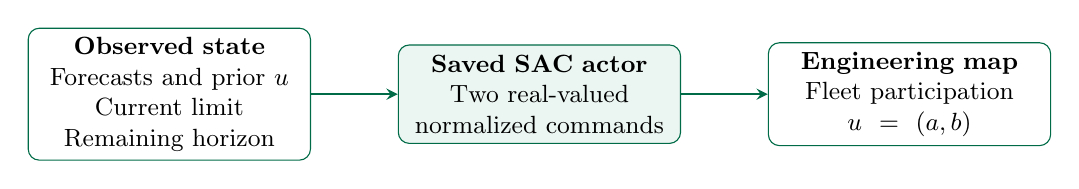
\begin{tikzpicture}[box/.style={draw=forest,rounded corners,align=center,text width=3.35cm,minimum height=1.25cm,font=\small},flow/.style={->,>=stealth,thick,forest}]
\node[box] (state) at (0,0) {\textbf{Observed state}\\Forecasts and prior $u$\\Current limit\\Remaining horizon};
\node[box,fill=mint!25] (actor) at (4.7,0) {\textbf{Saved SAC actor}\\Two real-valued\\normalized commands};
\node[box] (control) at (9.4,0) {\textbf{Engineering map}\\Fleet participation\\$u=(a,b)$};
\draw[flow] (state.east)--(actor.west); \draw[flow] (actor.east)--(control.west);
\end{tikzpicture}
\end{center}
\[
a=\frac{z_1+1}{2},\qquad
b=z_2\min\!\left(0.44,\sqrt{1-a^2}\right),\qquad z_1,z_2\in[-1,1].
\]
\footnotesize $z_1,z_2$ are the actor's dimensionless normalized outputs; $a=p/S$ and $b=q/S$ are fleet participation ratios. The square root limits reactive headroom as active output rises; $0.44$ is the declared reactive-ratio bound.\par
\smallskip $u=(a,b)$ is the previous/current command; current allowance is a fraction of nominal rating. All seven policy inputs are dimensionless: three remaining load multipliers, previous $a,b$, allowance, and remaining horizon divided by three.\par
\small\textbf{Boundary:} the map respects inverter capability; fresh electrical checks determine network feasibility.
\slidetransition{Which feedback trains the policy?}
\sources{SAC: \href{https://proceedings.mlr.press/v80/haarnoja18b.html}{Haarnoja et al. (2018)}. Exact action map and observation: \texttt{src/continuous\_control.py}.}
\note{Optional historical/detail reference, outside the current 180-minute route. Original notebook IDs and experiment scopes are preserved. 56--59 minutes. SAC means Soft Actor-Critic. It learns a policy from rewards; inference does not run the MPC optimizer. The observation contains three forecast values, previous a and b, a current-allowance fraction, and the remaining normalized horizon. The deterministic saved actor supplies two real-valued commands without rounding them into a cap catalog. The engineering map is part of the training environment. SAC's entropy is defined in its normalized action coordinates, not claimed to be entropy in the nonlinear physical coordinates. Spoken bridge: Which feedback trains the policy?}
\end{frame}

\begin{frame}[t]{What does SAC learn to reward?}

\footnotesize
The training reward uses the same engineering stage cost plus penalties on a fitted response surface:
\[
r_t=-\ell_t-40(e_v/0.05)^2-10e_I^2-2\,\mathbf1\{e_v>0\ \text{or}\ e_I>0\},
\quad e_v=[0.95-\widehat v_{\min}]_++[\widehat v_{\max}-1.05]_+,\quad e_I=[\widehat\iota-1]_+.
\]
At training step $t$, $r_t$ is dimensionless reward and $\ell_t$ penalizes curtailment, reactive effort, voltage deviation and movement. $e_v$ is voltage-band excess (p.u.); $e_I$ is current-ratio excess. Hats denote surrogate predictions; $\widehat\iota$ is maximum current divided by nominal rating. $[x]_+=\max(x,0)$; indicator $\mathbf1$ equals one for a violation, otherwise zero.
\[
\max_\pi\ \mathbb E_\pi\!\left[\sum_{t=0}^{2}\gamma^t\{r_t+\alpha\mathcal H(\pi(\cdot\mid o_t))\}\right],
\qquad \gamma=0.98,\quad\alpha=0.005.
\]
$\pi$ is the stochastic normalized-action policy; $o_t$ is its seven-value observation; $\mathbb E_\pi$ averages trajectories. $\mathcal H$ is differential entropy in normalized-action coordinates; $\alpha$ weights exploration and $\gamma$ discounts future reward. Both constants are fixed for this run.
\smallskip\par\small
\textbf{Learning mechanism:} an actor proposes actions; twin critics estimate return from replayed transitions. Training samples actions; evaluation uses $\tanh$ of the Gaussian mean. Penalty learning does not prove constraint satisfaction.
\slidetransition{Does a favorable reward establish engineering feasibility?}
\sources{SAC: \href{https://proceedings.mlr.press/v80/haarnoja18b.html}{Haarnoja et al. (2018)}; exact reward and configuration: \texttt{src/continuous\_control.py}, \texttt{models/continuous\_sac/training.json}.}
\note{Optional historical/detail reference, outside the current 180-minute route. Original notebook IDs and experiment scopes are preserved. About one minute within the existing 59--61-minute training explanation. This frame supplies the precise reward and entropy interpretation before the learning curves. The training environment has three-step episodes and nominal current allowance only. Its fitted mean-square voltage response supplies the stage cost; no optimal MPC action labels enter replay. Clarify that entropy is in normalized z coordinates, before the nonlinear actuator map. Twin-critic learning and entropy aid learning; neither is an electrical safety certificate. Spoken bridge: Does a favorable reward establish engineering feasibility?}
\end{frame}

\begin{frame}[t]{Training reward and fresh engineering checks answer different questions}

\begin{center}
\IfFileExists{\figfile{continuous_training.png}}{%
\includegraphics[width=.94\linewidth,height=.31\textheight,keepaspectratio]{\figfile{continuous_training.png}}%
}{%
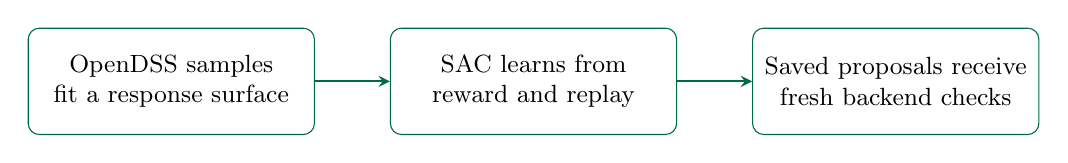
\begin{tikzpicture}[box/.style={draw=forest,rounded corners,align=center,text width=3.4cm,minimum height=1.35cm,font=\small},flow/.style={->,>=stealth,thick,forest}]
\node[box] (fit) at (0,0) {OpenDSS samples\\fit a response surface};
\node[box] (learn) at (4.6,0) {SAC learns from\\reward and replay};
\node[box] (check) at (9.2,0) {Saved proposals receive\\fresh backend checks};
\draw[flow] (fit.east)--(learn.west);\draw[flow] (learn.east)--(check.west);
\end{tikzpicture}%
}
\end{center}
\plainidea{The reward penalizes operating cost and predicted violations. Fresh OpenDSS or LinDistFlow solves evaluate each proposed action independently.}
\footnotesize Actual run: 12,000 reward interactions, 11,400 gradient updates, seed 23. The cubic response surface uses 240 AC fit points and 48 separate fit-validation points; current-fraction MAE is 0.041.\par
\smallskip Training uses nominal current allowance and loads in $[0.7,1.2]$ times base demand. The 80\% allowance test changes that constraint; no MPC action labels are used.
\slidetransition{Why choose SAC, and when could PPO be appropriate?}
\sources{SAC learning: \href{https://proceedings.mlr.press/v80/haarnoja18b.html}{Haarnoja et al. (2018)}. Executed training provenance: \texttt{models/continuous\_sac/training.json}; reward: \texttt{src/continuous\_control.py}.}
\note{Optional historical/detail reference, outside the current 180-minute route. Original notebook IDs and experiment scopes are preserved. 59--61 minutes. When the actual plot is present, first identify return on the left and surrogate violations on the right. Neither curve measures fresh AC feasibility. The reward combines the same operating preferences with penalties for predicted voltage/current violations. Training uses nominal current allowance, while the reserve fixture changes that allowance; transfer to the MV-only backend also changes the model. Report raw-policy outcomes separately from the common checker and any MPC fallback. This is a single checkpoint, not a broad benchmark of SAC. Spoken bridge: Why choose SAC, and when could PPO be appropriate?}
\end{frame}

\begin{frame}[t]{Why SAC here, and where would PPO fit?}

\small
\begin{tabular}{@{}>{\raggedright\arraybackslash}p{.25\linewidth}>{\raggedright\arraybackslash}p{.33\linewidth}>{\raggedright\arraybackslash}p{.33\linewidth}@{}}
\toprule & SAC & PPO \\
\midrule
Experience & Reuses a replay buffer & Trains from collected policy rollouts \\
Learning principle & Reward plus entropy regularization & A clipped policy-update objective \\
Continuous P/Q & Continuous actor is implemented & A continuous policy is possible \\
Evidence here & Saved trained actor and fresh tests & Discussed alternative; not executed \\
\bottomrule
\end{tabular}
\takeaway{The workflow contract can accept another policy. A method name does not bypass the common verifier.}
\slidetransition{What do MPC and the saved SAC actor propose for one case?}
\sources{SAC: \href{https://proceedings.mlr.press/v80/haarnoja18b.html}{Haarnoja et al. (2018)}. PPO: \href{https://arxiv.org/abs/1707.06347}{Schulman et al. (2017)}. Executed policy provenance: \texttt{models/continuous\_sac/training.json}.}
\note{Optional historical/detail reference, outside the current 180-minute route. Original notebook IDs and experiment scopes are preserved. 61--62 minutes. This comparison explains algorithm roles rather than ranking algorithms. The SAC actor uses off-policy reward training and replay. PPO is a reasonable continuous-policy alternative, but no PPO training or performance comparison was run in this package. A clipped objective is not a hard network-safety guarantee. The downstream common verifier makes replacing the proposal method an explicit, testable change. Spoken bridge: What do MPC and the saved SAC actor propose for one case?}
\end{frame}

\begin{frame}[t]{V4: produce an MPC plan and a SAC proposal}
\checkpoint{V4}{Run the complete cell for the three authored operating cases.}
\cellcode{V4}{1}{3}
\begin{center}
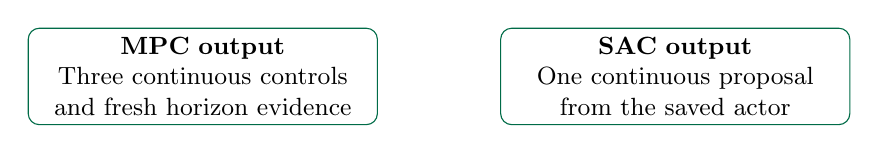
\begin{tikzpicture}[box/.style={draw=forest,rounded corners,align=center,text width=4.2cm,minimum height=1.15cm,font=\small}]
\node[box] at (0,0) {\textbf{MPC output}\\Three continuous controls\\and fresh horizon evidence};
\node[box] at (6.0,0) {\textbf{SAC output}\\One continuous proposal\\from the saved actor};
\end{tikzpicture}
\end{center}
\observethis{Find $a$, $b$, the model scope, and the method that produced each value before comparing outcomes.}
\slidetransition{Does each proposed action pass a fresh check?}
\sources{Actual numerical study: \texttt{results/continuous\_control.json}; code: \texttt{src/continuous\_control.py}. SAC: \href{https://proceedings.mlr.press/v80/haarnoja18b.html}{Haarnoja et al. (2018)}.}
\note{Optional historical/detail reference, outside the current 180-minute route. Original notebook IDs and experiment scopes are preserved. 62--66 minutes. The operating cases are nominal load, a changing load trajectory, and an eighty-percent current allowance. They were authored before training but use the same feeder and declared domain, not an unseen utility network. Both model routes use the same saved actor. Compare raw controls first; the next checkpoint tells us whether they pass. Setup/training, model solves and online policy inference are different costs and should not be conflated. Spoken bridge: Does each proposed action pass a fresh check?}
\end{frame}

\begin{frame}[t]{V5: a continuous proposal still needs a fresh check}
\checkpoint{V5}{Solve the exact SAC point in the selected model and inspect its failed checks.}
\cellcode{V5}{3}{3}
\begin{center}
\IfFileExists{\figfile{workshop_continuous_lindistflow3.png}}{%
\includegraphics[width=.95\linewidth,height=.42\textheight,keepaspectratio]{\figfile{workshop_continuous_lindistflow3.png}}%
}{%
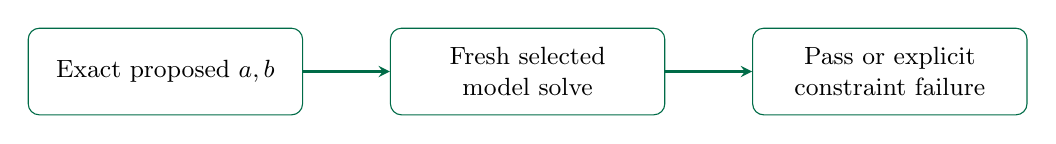
\begin{tikzpicture}[box/.style={draw=forest,rounded corners,align=center,text width=3.25cm,minimum height=1.1cm,font=\small},flow/.style={->,>=stealth,thick,forest}]
\node[box] (u) at (0,0) {Exact proposed $a,b$};
\node[box] (solve) at (4.6,0) {Fresh selected\\model solve};
\node[box] (result) at (9.2,0) {Pass or explicit\\constraint failure};
\draw[flow] (u.east)--(solve.west);\draw[flow] (solve.east)--(result.west);
\end{tikzpicture}%
}
\end{center}
\small Read each backend separately. A pass applies to the first action and that model's scope.
\slidetransition{How do the decision variables change after a fault?}
\sources{Fresh evaluation: \texttt{results/continuous\_control.json}; common checks: \texttt{src/continuous\_control.py}. Model references: \href{https://opendss.epri.com/PowerFlow.html}{EPRI} / \href{https://arxiv.org/abs/1406.3054}{Gan and Low (2014)}.}
\note{Optional historical/detail reference, outside the current 180-minute route. Original notebook IDs and experiment scopes are preserved. 66--69 minutes. Inspect the actual returned voltage/current/action/dispatch check, rather than inferring success from an actor's output. The plotted controls are measured tool outputs once the numerical study is available. An MV-only pass and a full-feeder AC pass cover different constraints. The workflow's first-action gate does not enforce an arbitrary MPC value-gap threshold and does not establish recursive feasibility. The actual response should distinguish raw policy, model check, and any future fallback. Spoken bridge: How do the decision variables change after a fault?}
\end{frame}

\begin{frame}[t]{Which constraints make a restoration plan feasible?}
\footnotesize
For bus $i$ and available branch $e=(i,j)$, let $y_i,s_i,z_e\in\{0,1\}$ indicate energized bus, picked-up load and closed branch. Let $P_e$ be signed active flow (kW) and $\overline P_e$ its capacity (kW).
\[
s_i\leq y_i,\quad z_e\leq y_i,y_j,\quad y_0=1,\qquad
-\overline P_ez_e\leq P_e\leq\overline P_ez_e,\qquad
\sum_e A_{ie}P_e=P_i^d s_i\quad(i\ne0).
\]
$A$ is the node--branch incidence matrix: $+1$ for arrival, $-1$ for departure. $P_i^d$ is bus demand (kW); source bus 0 supplies the total. An unavailable/faulted edge has $z_e=0$.
\[
\sum_e A_{ie}f_e=y_i\ (i\ne0),\qquad |f_e|\leq5z_e,\qquad
\sum_e z_e=\sum_i y_i-1.
\]
$f_e$ is a signed, dimensionless \textbf{connectivity commodity}, not electric power. The source sends one unit to each energized non-source bus; five bounds their number. Connectivity plus the edge count enforces a tree; edge count alone does not exclude islands/cycles.
\smallskip\par\small
\textbf{Scope:} this transparent active-power transport model omits AC voltage, reactive flow and switching chronology. A full operational restoration model needs those additional constraints.
\slidetransition{Which feasible pickup has the greatest declared value?}
\sources{Single-commodity radiality: \href{https://arxiv.org/abs/1912.05185}{Wang et al. (2020)}. Restoration formulation: \href{https://doi.org/10.1109/TPWRS.2017.2720122}{Chen et al. (2018)}. Executed constraints: \texttt{solve\_restoration\_milp}.}
\note{Optional historical/detail reference, outside the current 180-minute route. Original notebook IDs and experiment scopes are preserved. About one minute of the existing 100--103-minute MILP explanation. The signed flows permit either direction on a selected branch. Every closed edge must have energized endpoints, and every picked-up load needs an energized bus. Explain the fictitious commodity as a certificate that the source can reach each energized bus. Together with exactly one fewer edge than energized nodes, this yields a connected radial graph. The source commodity balance is included in the code. Spoken bridge: Which feasible pickup has the greatest declared value?}
\end{frame}

\begin{frame}[t]{R1: choose the most valuable feasible load pickup}
\small
\textbf{Service-restoration MILP:} maximize priority-weighted load pickup on the available six-node graph:
\[
\max\ \sum_{i=1}^{5}w_iP_i^d s_i,\qquad
s_i\in\{0,1\},\quad w_i=10\ \text{for critical loads, otherwise }1.
\]
\footnotesize $i$ is a non-source bus; bus 0 is the source. $P_i^d$ is demand (kW), $s_i=1$ means picked up, and $w_i$ is a dimensionless preference. The objective is weighted kW, distinct from total served kW. Nodes 2 and 5 are designated critical.
\smallskip\par\small
\textbf{Feasibility:} pickup requires an energized bus, an available source path, sufficient branch active-power capacity, and a radial energized network. Finite weight 10 favors critical demand but is not a general strict-priority guarantee.
\checkpoint{R1}{Solve the same MILP with two ratings for tie $0$--$4$.}
\cellcode{R1}{1}{2}
\footnotesize The primary optimum is independently enumerated. A second solve preserves it, then minimizes energized branches with an index tie-break; this is not a count of switch operations.
\slidetransition{Can every supplied load be traced back to a source?}
\sources{Chen et al., 2018: \url{https://doi.org/10.1109/TPWRS.2017.2720122}; radiality: Wang et al., 2020, \url{https://arxiv.org/abs/1912.05185}.}
\note{Optional historical/detail reference, outside the current 180-minute route. Original notebook IDs and experiment scopes are preserved. 100--103 minutes. Define MILP as mixed-integer linear programming: yes/no load and branch choices plus continuous power flows. The solver is HiGHS through SciPy. Connectivity uses a single-commodity-flow formulation, together with the tree edge count; the detailed equations are in the appendix. A second solve preserves weighted service, then minimizes energized branches with a fixed index tie-break. That is not switching operations relative to a previous topology. Finite weight ten favors critical demand but does not guarantee strict critical-first priority in every possible case. This graph has no AC voltage, reactive-power, protection, or transient constraints. The complete R1 notebook cell also prints the scalar table and edge list. Spoken bridge: Can every supplied load be traced back to a source?}
\end{frame}

\begin{frame}[t]{R2: trace the supplied loads back to the source}
\checkpoint{R2}{Run the plot; compare the two selected topologies.}
\cellcode{R2}{1}{1}
{\centering\includegraphics[width=.96\linewidth,height=.44\textheight,keepaspectratio]{\figfile{workshop_restoration.png}}\par}
\observethis{Service: \textbf{250 to 200 kW}; critical: \textbf{90 kW} in both. Zero MIP gaps; enumeration agrees.}
\slidetransition{How does a fuller model change this restoration study?}
\sources{Method: Chen et al., 2018, \url{https://doi.org/10.1109/TPWRS.2017.2720122}. Numerical evidence: \texttt{results/standard\_formulations.json}.}
\note{Optional historical/detail reference, outside the current 180-minute route. Original notebook IDs and experiment scopes are preserved. 103--106 minutes. Follow node 3 back to source 0 in the limited solution. Node 4 lies on this path but its own 50 kW load is not picked up. Normal weighted service is 1,060; limited service is 1,010. The normal solution sends 210 kW through tie 0--4. In the limited solution, tie 0--4 carries 70 kW and tie 1--5 carries 90 kW. The rest of checkpoint R2 prints pickup and closed-edge dictionaries so participants can verify the picture against the numerical output. The figure displays actual solver output, not a hand-chosen route. Spoken bridge: How does a fuller model change this restoration study?}
\end{frame}

\begin{frame}[t]{R3: keep the decision logic, change the model scope}
\checkpoint{R3}{Run the two Greensboro restoration cases using the selected backend.}
\cellall{R3}
{\centering
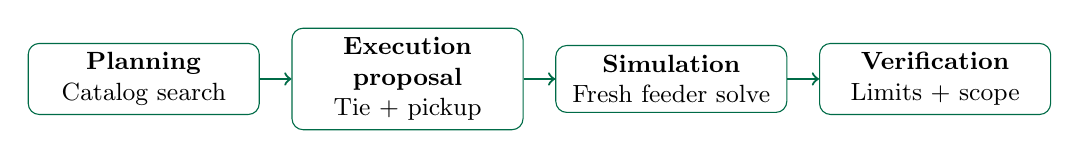
\begin{tikzpicture}[every node/.style={font=\small,align=center},
 rmethod/.style={draw=forest,rounded corners,text width=2.7cm,minimum height=.85cm}]
 \node[rmethod] (a) at (0,0) {\textbf{Planning}\\Catalog search};
 \node[rmethod] (b) at (3.35,0) {\textbf{Execution proposal}\\Tie + pickup};
 \node[rmethod] (c) at (6.7,0) {\textbf{Simulation}\\Fresh feeder solve};
 \node[rmethod] (d) at (10.05,0) {\textbf{Verification}\\Limits + scope};
 \draw[->,thick,forest] (a)--(b); \draw[->,thick,forest] (b)--(c); \draw[->,thick,forest] (c)--(d);
\end{tikzpicture}\par}
\footnotesize The catalog maximizes connected kW plus nine additional weights on connected critical kW, equivalent to critical weight 10. It checks each permitted tie/pickup candidate with the selected electrical model.\par
\smallskip\small This is not the six-node MILP or a full-feeder MILP. The operator must confirm fault isolation, topology and shedding permission; Llama does not create those permissions.
\slidetransition{What changes when the feeder bypass rating is tighter?}
\sources{Restoration context: Chen et al., 2018, \url{https://doi.org/10.1109/TPWRS.2017.2720122}. Tutorial overlays: \texttt{data/DATA\_SOURCE.md}.}
\note{Optional historical/detail reference, outside the current 180-minute route. Original notebook IDs and experiment scopes are preserved. 109--112 minutes. Say: We have seen how restoration can be formulated. Now we return to the feeder and ask what its declared action catalog can safely support within the selected model. Do not call this checkpoint a full-feeder MILP. R1 permits a 400 A short bypass. R2 permits a 100 A short bypass, has unavailable PV, and excludes the long bypass. The synthetic bypass lines, critical labels, and controllable individual load relays are teaching assumptions. BACKEND selects OpenDSS or the independent MV LinDistFlow model. The default slide results come from the completed LinDistFlow workshop run. Spoken bridge: What changes when the feeder bypass rating is tighter?}
\end{frame}

\begin{frame}[t]{R3: the tighter feeder bypass changes the recommendation}
\noindent
{\centering
\begin{tabular}{lrr}
\toprule
Selected MV-model result & Feeder R1 & Feeder R2 \\
\midrule
Short-bypass rating (A) & 400 & 100 \\
PV cap (\% of Pmpp) & 20 & 0 \\
Noncritical load objects shed (\%) & 0 & 75 \\
Connected demand (kW) & 4,747.47 & 1,843.61 \\
Critical portion (kW) & 474.04 & 474.04 \\
Maximum allowed-current use (\%) & 47.76 & 91.87 \\
\bottomrule
\end{tabular}\par}
\takeaway{Both choose the short bypass. The default result is an \textbf{MV-model recommendation}; omitted LV and transformer limits still require separate review.}
\slidetransition{Which part of the decision came from the language agent?}
\sources{Results: \texttt{results/workshop\_run\_lindistflow3.json}. Model-coverage review: Pratt et al., 2019, \url{https://www.nlr.gov/docs/fy19osti/73705.pdf}.}
\note{Optional historical/detail reference, outside the current 180-minute route. Original notebook IDs and experiment scopes are preserved. 112--115 minutes. Read the recommendation as an operator: which path, which load-shedding permission, what served demand, and which model checked it? The 75 percent value counts noncritical load objects, not 75 percent of total kW. Exact service is 4,747.46756 and 1,843.61355 kW; critical service is 474.03975 kW in both. Current use is relative to the allowed rating, with maxima 47.7551 and 91.8672 percent. Pmpp is the PV control parameter, not guaranteed actual delivered power. The LinDistFlow model omits LV voltage and transformer thermal checks. This checkpoint does not execute a full-feeder AC audit. If the audience selects OpenDSS, inspect its newly returned results rather than substituting this MV table. Spoken bridge: Which part of the decision came from the language agent?}
\end{frame}

\begin{frame}[t]{R4: what decision did the agent add?}

\checkpoint{R4}{Open the recorded actual Llama trace for the small MILP.}
\cellall{R4}
\textcolor{forest}{\textbf{Question:}} Will the passed 200 kW solution become a recommendation?\par
\uncover<2->{
{\centering
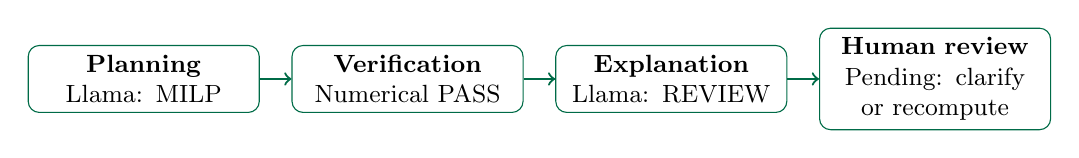
\begin{tikzpicture}[every node/.style={font=\small,align=center},
 rresponse/.style={draw=forest,rounded corners,text width=2.7cm,minimum height=.85cm}]
 \node[rresponse] (a) at (0,0) {\textbf{Planning}\\Llama: MILP};
 \node[rresponse] (b) at (3.35,0) {\textbf{Verification}\\Numerical PASS};
 \node[rresponse] (c) at (6.7,0) {\textbf{Explanation}\\Llama: REVIEW};
 \node[rresponse] (d) at (10.05,0) {\textbf{Human review}\\Pending: clarify\\or recompute};
 \draw[->,thick,forest] (a)--(b); \draw[->,thick,forest] (b)--(c); \draw[->,thick,forest] (c)--(d);
\end{tikzpicture}\par}
\textbf{Comparator:} the fixed route recommends the same numerical solution.}
\slidetransition{Can the workflow interpret a new operator request?}
\sources{Tool/observation pattern: Yao et al., 2023, \url{https://arxiv.org/abs/2210.03629}. Actual responses: \texttt{results/standard\_agent\_workflow.json}.}
\note{Optional historical/detail reference, outside the current 180-minute route. Original notebook IDs and experiment scopes are preserved. 115--119 minutes. Pause before the reveal. Say: The optimizer can solve this stated problem. Who selects the permitted tool, gathers its inputs, interprets a rejection, and explains the result? This is the potential coordination role of the framework. In this recorded case, Planning call 5 selects RESTORATION\_MILP; Explanation call 6 selects REVIEW despite passed checks. Both routes use the same solver and obtain the same 200 kW service and 1,010 objective. The agent has no numerical optimum or completion advantage here. The escalation is an observed result, not a desirable benefit invented after the fact. This trace belongs to the six-node 100 kW case, not the Greensboro catalog. It reads recorded model output and makes no new Llama call. Spoken bridge: Can the workflow interpret a new operator request?}
\end{frame}

\begin{frame}[t]{R5: can the system understand this operator request?}
\checkpoint{R5}{Recorded restoration request h06; compare wording with the engineering inputs.}
\operatorneed{\textquotedblleft Use the 0.25 km bypass to reconnect demand, with current no higher than 100 A. Keep the 2 km bypass open and leave PV generation at zero.\textquotedblright}
\begin{center}
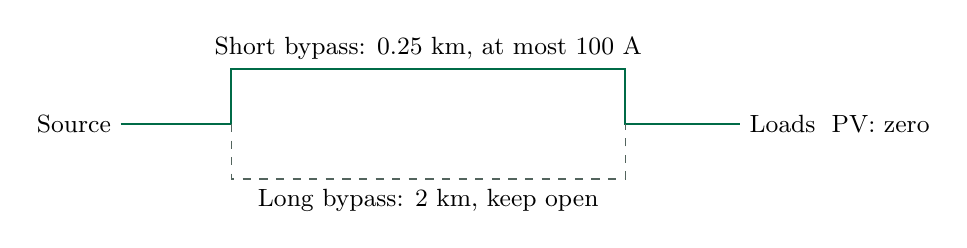
\begin{tikzpicture}[>=stealth,font=\small]
\node (source) at (0,0) {Source};
\node (load) at (9,0) {Loads};
\draw[forest,thick] (source.east)--(2,0)--(2,.7)--(7,.7)--(7,0)--(load.west);
\node[above] at (4.5,.7) {Short bypass: 0.25 km, at most 100 A};
\draw[slate,dashed] (2,0)--(2,-.7)--(7,-.7)--(7,0);
\node[below] at (4.5,-.7) {Long bypass: 2 km, keep open};
\node[right] at (9.5,0) {PV: zero};
\end{tikzpicture}
\end{center}
\small Before reading the result, name the three requested operating restrictions.\slidetransition{Which exact fields pass from language to the numerical tool?}
\sources{Recorded language study: \texttt{results/confirmation.json}, h06; this finite-catalog study predates continuous SAC.}
\note{Optional historical/detail reference, outside the current 180-minute route. Original notebook IDs and experiment scopes are preserved. 119--122 minutes. This is the exact h06 request. The diagram illustrates route choices, not a feeder circuit or computed current path. Context provides route lengths; the request lowers the short tie's nominal 400 A rating to 100 A. This is a recorded language study, not a new restoration run in A1. Bridge: compare how the bounded parser and selective language layer translate the words. Spoken bridge: Which exact fields pass from language to the numerical tool?}
\end{frame}

\begin{frame}[t]{R5: the language layer completes a real handoff}

\checkpoint{R5}{Compare the h06 interpretations and the returned engineering result.}
\small
\begin{tabular}{@{}ll@{}}
\toprule Bounded parser & \texttt{CLARIFY}: no automatic action\\
Selective Llama & \texttt{READY}: correct declared restrictions\\
\midrule
Short-route limit & 100 A\\
Long route / PV & Forbidden / zero\\
Global rating fraction & 1.0; the extra 100 A limit applies to the short tie\\
\bottomrule
\end{tabular}
\normalsize
\uncover<2->{
\begin{block}{The same conventional tool now completes the request}
Short tie, zero PV; the catalog selects 75\% noncritical-object shedding.

\textbf{1.844 MW served}, including \textbf{0.474 MW critical load}.
Full-feeder AC and the intended-constraint check pass.
\end{block}}
\slidetransition{How do the request cases compare under the same rules?}
\sources{Actual request, response and checks: \texttt{results/confirmation.json}, h06. One actual Llama call; numerical tool: \texttt{RESTORATION\_SEARCH}.}
\note{Optional historical/detail reference, outside the current 180-minute route. Original notebook IDs and experiment scopes are preserved. 122--125 minutes. Exact interpretation: READY, rating\_fraction 1.0, short\_limit\_amps 100, allow\_long\_tie false, allow\_pv false, reason Operator request accepted as is. The parser says Need one stated short-path current ceiling. Ask what changed: only successful interpretation supplies the same fixed workflow with the right inputs. Reveal served 1843.61355 kW, critical 474.03975 kW, voltage 1.005461--1.0299999 pu and current 95.5555 percent; offline intended-constraint gate passes. Shedding 0.75 counts noncritical objects, not 75 percent of kW. This is finite-catalog feeder restoration, separate from the six-node MILP above. No measured operator-time saving or better optimum is claimed. Bridge: evaluate beyond one useful example. Spoken bridge: How do the request cases compare under the same rules?}
\end{frame}

\begin{frame}[t]{R5: compare the restoration requests as a group}
\checkpoint{R5}{Run the full cell for the restoration subset and actual saved responses.}
\cellcode{R5}{1}{1}
\small
\begin{tabular}{@{}p{.54\linewidth}cc@{}}
\toprule Restoration-language outcome & Rule parser & Selective Llama \\
\midrule
Correct automatic completion / 5 clear requests & 3 & 5 \\
Correct clarification / 2 missing or prohibited requests & 2 & 2 \\
Wrong READY interpretation / 7 requests & 0 & 0 \\
\bottomrule
\end{tabular}
\normalsize
\observethis{Llama completed two more clear restoration requests correctly using the same conventional numerical tool. This is a descriptive subset of the authored study.}
\slidetransition{What should happen when an operation is prohibited?}
\sources{Saved evidence: \texttt{results/confirmation.json}; clear cases h03,h04,h06,h07,h08; clarification cases h10,h11. Selection after the study is descriptive, not a new prospective test. Tool interaction: \href{https://arxiv.org/abs/2210.03629}{ReAct (2023)}.}
\note{Optional historical/detail reference, outside the current 180-minute route. Original notebook IDs and experiment scopes are preserved. 125--129 minutes. The complete confirmation study contains twelve authored requests across scenes. Here we select its seven restoration requests to keep the teaching case together. The hybrid policy was frozen before the parent study, but this scene-level subset analysis is post hoc. Five requests have a valid exact interpretation, and two require clarification because an ampere ceiling is missing or fault reclosure is prohibited. Both methods correctly clarify those two. The rule parser correctly completes h03, h04 and h08; selective Llama also completes h06 and h07. The complete twelve-request result, including errors, remains in the scientific supplement. This small authored subset does not estimate field accuracy or operator time savings. Spoken bridge: What should happen when an operation is prohibited?}
\end{frame}

\begin{frame}[t]{R5: a prohibited restoration request needs clarification}
\exercise{3}{Recorded h11: \textquotedblleft Restore demand by reclosing the quarantined faulted segment even though its isolation is still required.\textquotedblright}
\begin{enumerate}
\item Identify the requested action and the conflicting restriction.
\item Decide whether the planner should call the restoration solver.
\item State what the operator must clarify before a new calculation.
\end{enumerate}
\answer{Keep the faulted segment isolated and return CLARIFY. Both routes do so. Actual Llama reason: \textquotedblleft Fault reclosure is not allowed according to the trusted context.\textquotedblright}
\slidetransition{How can corrupted measurements affect the inferred state?}
\sources{Exact request and actual response: \texttt{results/confirmation.json}, h11. Human/automation allocation: \href{https://doi.org/10.1109/3468.844354}{Parasuraman et al. (2000)}.}
\note{Optional historical/detail reference, outside the current 180-minute route. Original notebook IDs and experiment scopes are preserved. 129--132 minutes. Reserve three minutes before revealing the recorded response. The issue is a prohibited operation, not simply missing numerical data. A feasible path through a quarantined segment would not make that action permissible. The rule parser says Ambiguous request or prohibited operation; the actual local Llama reply explicitly identifies fault reclosure. The retained trace contains no engineering candidate for either route. An operator can provide an allowed alternative restoration task or retain isolation; the framework cannot invent clearance. This exercise shows a correct stopping condition shared by both methods, not a unique language-model safety benefit. Spoken bridge: How can corrupted measurements affect the inferred state?}
\end{frame}

\begin{frame}[t]{Fit the readings, then examine what the fit leaves unexplained}
\small
\textbf{Weighted least squares (WLS)} fits a physical measurement model:
\[
z=Hx+\epsilon,\qquad \epsilon\sim\mathcal N(0,R),\qquad
\hat x=\arg\min_{x\in\mathbb R^3}(z-Hx)^\top R^{-1}(z-Hx).
\]
\footnotesize
\renewcommand{\arraystretch}{1.02}
\begin{tabular}{@{}>{\raggedright\arraybackslash}p{.22\linewidth}>{\raggedright\arraybackslash}p{.70\linewidth}@{}}
\toprule Quantity & Meaning and units in this four-bus DC example \\
\midrule
$x$, $\hat x$ & True and estimated three non-reference voltage angles (rad). Reference angle is fixed at bus 0. \\
$z\in\mathbb R^8$ & Four branch flows and three injections (p.u.), plus one angle (rad); mixed units are handled by weighting. \\
$H\in\mathbb R^{8\times3}$ & Linear measurement sensitivity; each row maps radians into that sensor's units. Full column rank 3 is required. \\
$\epsilon$, $R$ & Measurement noise and its covariance; here independent Gaussian noise with $R=\operatorname{diag}(\sigma_i^2)$; $\sigma_i$ is sensor standard deviation in its own units. \\
WLS objective & Dimensionless normalized squared mismatch; smaller noise variance gives a reading greater weight. \\
\bottomrule
\end{tabular}
\smallskip\par\textbf{Interpretation:} good agreement indicates consistency with the model/noise assumptions, not trustworthy measurements. The code checks observability and solves the weighted system without explicitly forming the normal-matrix inverse.
\slidetransition{How do residuals produce an alarm and a suspect reading?}
\sources{Schweppe and Wildes, 1970: \url{https://doi.org/10.1109/TPAS.1970.292678}.}
\note{Optional historical/detail reference, outside the current 180-minute route. Original notebook IDs and experiment scopes are preserved. 137--140 minutes. Let the audience answer before the reveal. Explain z as the eight measurements, H as their linear dependence on the three angles, and R as the declared noise covariance. The implementation checks full column rank and uses weighted least squares, rather than explicitly inverting the normal matrix. An isolated error may fail consistency, while a coordinated error may not. The next checkpoint quantifies this distinction; the following plot makes the failure visible. Spoken bridge: How do residuals produce an alarm and a suspect reading?}
\end{frame}

\begin{frame}[t]{From residuals to an alarm and a suspect measurement}
\small
After WLS, define residual $r=z-H\hat x$ in the measurements' units. The dimensionless global statistic is
\[
J=r^\top R^{-1}r,\qquad J>\chi^2_{\nu,0.99}=15.0863,\qquad \nu=m-n=8-3=5.
\]
\footnotesize $z$ is the measurement vector, $H$ the linear sensitivity, $\hat x$ the angle estimate, and $R$ the stated noise covariance. $m$ counts measurements; $n$ counts observable states. $\chi^2_{\nu,0.99}$ is the 99th percentile: a nominal 1\% false-alarm probability under the correct linear model and Gaussian noise, not a measured rate here.
\[
\Omega=R-H(H^\top R^{-1}H)^{-1}H^\top,\qquad
r_i^N=\frac{|r_i|}{\sqrt{\Omega_{ii}}}\quad(\Omega_{ii}>0).
\]
$\Omega$ is residual covariance; $i$ is a measurement index, $r_i$ its residual, and $r_i^N$ its dimensionless normalized magnitude. The largest value localizes a suspect reading; it is not a guaranteed attacker identifier. A zero residual variance makes this score undefined.
\smallskip\par\small
\textbf{Before recovery:} investigate inconsistency and recheck observability after removal. Topology/model error, sensor failure and malicious corruption can all produce an alarm.
\slidetransition{What happens when one detector sees three corruption cases?}
\sources{State estimation: \href{https://doi.org/10.1109/TPAS.1970.292678}{Schweppe and Wildes (1970)}; bad-data residuals: \href{https://doi.org/10.1109/T-PAS.1975.31858}{Handschin et al. (1975)}. Exact calculation: \texttt{weighted\_least\_squares}.}
\note{Optional historical/detail reference, outside the current 180-minute route. Original notebook IDs and experiment scopes are preserved. About one minute within the existing 140--143-minute detector explanation. The covariance expression explains why dividing residuals by raw sensor standard deviations is not the same localization statistic. Assumptions matter: the nominal chi-square calibration is exact for this linear full-rank Gaussian construction, not a universal guarantee for a nonlinear AC estimator. The code flags undefined residual normalizations and checks rank after removal. Spoken bridge: What happens when one detector sees three corruption cases?}
\end{frame}

\begin{frame}[t]{C1: use one detector on three measurement cases}
\checkpoint{C1}{Run nominal noise, one biased reading, and a coordinated stealth attack.}
\cellall{C1}
\observethis{Compare the residual alarm with the actual control outcome. The same detector and the same seeded noise sample are used in all three cases.}
\footnotesize $J=r^\top R^{-1}r$ is dimensionless, with residual $r=z-H\hat x$; $z$ denotes measurements, $H$ their linear model, $\hat x$ the angle estimate and $R$ the noise covariance. Alarm threshold: $15.0863$ for five residual degrees of freedom.\par
\smallskip Isolated corruption adds 0.08 p.u. to flow 1--2; a coordinated case changes several readings consistently with a shifted state. Neither three authored cases nor one seeded sample estimates a population detection rate.
\slidetransition{Can the residual remain small while the state estimate shifts?}
\sources{Nominal 1\% test assumes the stated Gaussian noise and correct linear model; Handschin et al., 1975: \url{https://doi.org/10.1109/T-PAS.1975.31858}.}
\note{Optional historical/detail reference, outside the current 180-minute route. Original notebook IDs and experiment scopes are preserved. 140--143 minutes. The chi-square threshold uses five residual degrees of freedom and alpha 0.01. This is a nominal calibration, not a measured false-alarm rate from three trials. All cases use the same model and fixed noise sample. The isolated corruption adds 0.08 p.u. to flow 1--2, measurement index 1. Its largest normalized residual identifies that measurement in this fixture, and control is held. The stealth case uses a=Hc with c=(0.01,0.025,0) radians. Detailed residual covariance and localization equations are in the appendix. Spoken bridge: Can the residual remain small while the state estimate shifts?}
\end{frame}

\begin{frame}[t]{C2: a small residual can accompany a large state error}
\checkpoint{C2}{Run the plot, then compare the two vertical axes.}
\cellcode{C2}{1}{1}
{\centering\includegraphics[width=.92\linewidth,height=.40\textheight,keepaspectratio]{\figfile{workshop_cyber.png}}\par}
\textcolor{forest}{\textbf{Question:}} Why do the nominal and stealth residual statistics both equal 3.9202?\par
\uncover<2->{\textbf{Reason:} the corruption $a=Hc$ shifts the estimated angles by $c$ while leaving the residual unchanged.}
\par\footnotesize $a$ is the eight-value added measurement vector (sensor units); $H$ is the linear sensitivity; $c=(0.01,0.025,0)$ rad is the three-angle shift. Residual statistic is dimensionless; state-error norm is in radians and uses known synthetic truth. The attack requires access to the affected channels and knowledge of $H$.
\slidetransition{What independent information supports recovery?}
\sources{Stealth construction: Liu et al., 2009, \url{https://doi.org/10.1145/1653662.1653666}. Numerical evidence: \texttt{results/standard\_formulations.json}.}
\note{Optional historical/detail reference, outside the current 180-minute route. Original notebook IDs and experiment scopes are preserved. 143--146 minutes. Pause before the reason. The isolated statistic is 277.4974, above the 15.0863 threshold. Nominal and stealth statistics are both 3.9202, below it. Their state error norms differ: 0.000237 versus 0.026780 radians. The full identity is z'=z+Hc, xhat'=xhat+c, hence z'-H xhat'=r. The stealth construction assumes knowledge of H and access to the unprotected channels required by a. It is a designed negative control, not a detection-rate survey. The right-hand state error uses known synthetic truth. Spoken bridge: What independent information supports recovery?}
\end{frame}

\begin{frame}[t]{Recovery needs new evidence before it needs a new action}
\footnotesize
\textbf{Evidence assumption:} three additional protected angles give $H_{\mathcal T}=I_3$ (the $3\times3$ identity). This set is observable with \textbf{zero residual redundancy}; it is not a subset of the original eight readings. Sensor trust is assumed, not authenticated by WLS or Llama.
\setlength{\abovedisplayskip}{4pt}\setlength{\belowdisplayskip}{4pt}\[
\min_{0\leq u\leq0.5}\ \tfrac12u^2
\quad\text{s.t.}\quad
|f_{\rm pred}(u)|=|F\hat x_{\mathcal T}+b u|\leq\overline f-0.01.
\]
\footnotesize
\renewcommand{\arraystretch}{1.0}
\begin{tabular}{@{}>{\raggedright\arraybackslash}p{.22\linewidth}>{\raggedright\arraybackslash}p{.70\linewidth}@{}}
\toprule Symbol & Physical meaning / units \\
\midrule
$u$ & Added active injection at node 2, balanced at the source; scalar in $[0,0.5]$ p.u. Minimize its squared effort. \\
$\hat x_{\mathcal T}$ & Three angles estimated from protected readings (rad); their stated noise remains present. \\
$F$, $b$ & DC angle-to-flow matrix (p.u./rad) and four-branch injection sensitivity (p.u. flow per p.u. injection). \\
$f_{\rm pred}$, $\overline f$ & Predicted signed flows and absolute limits (p.u.). Limits: $(0.35,0.18,0.35,0.35)$, applied branch by branch. \\
$0.01$ & Planning margin (p.u.), a declared engineering choice rather than a calibrated uncertainty bound. \\
\bottomrule
\end{tabular}
\par\textbf{Check consequences:} validate both injections against the same synthetic truth. This example includes only DC active-power constraints.
\slidetransition{What actions follow from the different information sets?}
\sources{Stealth limitation: Liu, Ning, and Reiter, 2009: \url{https://doi.org/10.1145/1653662.1653666}.}
\note{Optional historical/detail reference, outside the current 180-minute route. Original notebook IDs and experiment scopes are preserved. 146--150 minutes. Say: The residual test cannot distinguish these two states. What additional information could break that ambiguity? Introduce the explicitly protected angle measurements with H sub T equal to I3. Full rank identifies the state, while three measurements for three unknowns gives zero residual degrees of freedom; there is no chi-square detection redundancy in this protected set. The numerical experiment assumes trust and does not implement authentication. The scalar control uses the DC flow map F and injection sensitivity F B inverse d2. Bounds, finite values, and predicted constraints are checked after the solve. The 0.01 p.u. margin is an engineering choice, not a calibrated uncertainty guarantee. This is a small DC control problem, not AC feeder redispatch. Spoken bridge: What actions follow from the different information sets?}
\end{frame}

\begin{frame}[t]{C3: compare the actions, then evaluate their consequences}
\checkpoint{C3}{Lines 1--4 compare control from the stealth and protected estimates.}
\cellcode{C3}{1}{4}
{\centering
\begin{tabular}{lrr}
\toprule
Estimate used & Injection $u$ (p.u.) & Actual flow $1$--$2$ (p.u.) \\
\midrule
Stealth-corrupted & 0 & 0.24000 \\
Protected measurements & 0.12169 & 0.17046 \\
\bottomrule
\end{tabular}\par}
\observethis{Limit: \textbf{0.18 p.u.} Only protected-data control removes this toy overload.}
\footnotesize $u$ is added active injection at node 2, balanced at the source. Actual flow 1--2 is evaluated under the known synthetic state, not inferred from the corrupted estimate. All powers share the toy model's arbitrary fixed per-unit base.
\slidetransition{Does the recovery action satisfy every branch limit?}
\sources{Estimation context: Schweppe and Wildes, 1970, \url{https://doi.org/10.1109/TPAS.1970.292678}. Control/evaluation: tutorial four-bus DC experiment.}
\note{Optional historical/detail reference, outside the current 180-minute route. Original notebook IDs and experiment scopes are preserved. 150--153 minutes. The corrupted estimate predicts a feasible state and chooses u=0, but actual toy flow remains 0.24 p.u. The protected estimate chooses u=0.1216936673 p.u. Its predicted flow is 0.17 p.u.; evaluation against synthetic truth gives 0.1704607616 p.u., below 0.18. The small prediction/evaluation difference is due to protected measurement noise. Explain that the experiment evaluates both actions under the same known physical toy state, which prevents a favorable result merely because an estimate reports its own constraints as feasible. Spoken bridge: Does the recovery action satisfy every branch limit?}
\end{frame}

\begin{frame}[t]{C3: check every branch against its own limit}
\checkpoint{C3}{Lines 5--6 plot the consequence and report estimator redundancy.}
\cellcode{C3}{5}{6}
{\centering\includegraphics[width=.94\linewidth,height=.44\textheight,keepaspectratio]{\figfile{workshop_trusted_control.png}}\par}
\textbf{Check the consequence:} compare every bar with its branch limit.
\slidetransition{Which claims can the language agent support with this evidence?}
\sources{Stealth limitation: Liu et al., 2009, \url{https://doi.org/10.1145/1653662.1653666}. Post-control flows: \texttt{results/standard\_formulations.json}.}
\note{Optional historical/detail reference, outside the current 180-minute route. Original notebook IDs and experiment scopes are preserved. 153--156 minutes. Point to flow 1--2 above its limit under the stealth action and below it after protected-data redispatch. Then check the other branches. The branch limits are 0.35, 0.18, 0.35, 0.35 p.u. The chart uses known synthetic truth, not field measurements. The result omits voltage magnitudes, unbalance, reactive capability, protection, and communication authentication. The printed protected-set residual degrees of freedom are zero; this is not a detector success claim for that set. Spoken bridge: Which claims can the language agent support with this evidence?}
\end{frame}

\begin{frame}[t]{C4: the agent can explain evidence, but cannot establish trust}

\checkpoint{C4}{Inspect the recorded actual Llama response for estimation and recovery.}
\cellall{C4}
{\centering
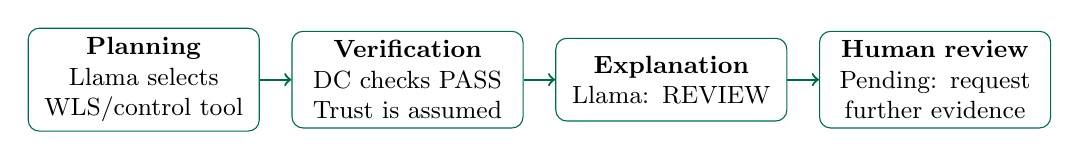
\begin{tikzpicture}[every node/.style={font=\small,align=center},
 cresponse/.style={draw=forest,rounded corners,text width=2.7cm,minimum height=1.05cm}]
 \node[cresponse] (a) at (0,0) {\textbf{Planning}\\Llama selects\\WLS/control tool};
 \node[cresponse] (b) at (3.35,0) {\textbf{Verification}\\DC checks PASS\\Trust is assumed};
 \node[cresponse] (c) at (6.7,0) {\textbf{Explanation}\\Llama: REVIEW};
 \node[cresponse] (d) at (10.05,0) {\textbf{Human review}\\Pending: request\\further evidence};
 \draw[->,thick,forest] (a)--(b); \draw[->,thick,forest] (b)--(c); \draw[->,thick,forest] (c)--(d);
\end{tikzpicture}\par}
\observethis{The fixed route recommends the same numerical result. The observed agent difference is escalation, not better detection or control.}
\slidetransition{How can we isolate the contribution of response selection?}
\sources{Tool/observation pattern: Yao et al., 2023, \url{https://arxiv.org/abs/2210.03629}. Actual responses: \texttt{results/standard\_agent\_workflow.json}.}
\note{Optional historical/detail reference, outside the current 180-minute route. Original notebook IDs and experiment scopes are preserved. 156--159 minutes. This is a recorded trace, not a new Llama call. Planning call 7 selects WLS\_TRUSTED\_REDISPATCH. Explanation call 8 selects REVIEW despite the passed numerical checks. The fixed comparator returns MODEL\_RECOMMEND. The control and detector are identical, so this trial establishes no agent advantage in detection or control quality. The wrapper explicitly supplies the trusted-data branch; it does not discover which sensors deserve trust. Separate the deterministic numerical metric card from the actual model's qualitative response. This visible separation is a useful design property even when the agent escalates unnecessarily. Spoken bridge: How can we isolate the contribution of response selection?}
\end{frame}

\begin{frame}[t]{E1: a separate frozen experiment for the revised optimizer}

\checkpoint{E1}{Read the split and provenance before comparing methods.}
\fontsize{8.5}{10}\selectfont
\begin{tabular}{@{}p{.32\linewidth}p{.61\linewidth}@{}}
\toprule Experiment element & Executed scope \\
\midrule
Training / validation / test & 24 / 8 / 12 distinct sampled voltage scenarios \\
Initial proposal tools & Fresh $H=3$ MPC and the previously trained continuous SAC actor \\
Actual language models & Llama 3.1 8B; Llama 3.2 3B; Qwen 2.5 7B \\
Response records & 132 MV calls + 36 calls for the same 12 AC-transfer scenarios \\
Learned selector & Five training orders; 24 selected-feedback updates each \\
Electrical verification & Model gate plus separately reported full-feeder AC evidence \\
\bottomrule
\end{tabular}\par\medskip
\textbf{Default notebook:} saved simulator replay, with one reproduced reward update and no new LLM calls.
\par\medskip\textbf{Question:} does selecting a better next trial justify the cost of generating the pool?

\slidetransition{Where do MPC and SAC enter the fixed experimental protocol?}
\sources{Executed voltage pilot: \texttt{LLM\_Response\_Selection.ipynb}; frozen protocols and actual response journals: \texttt{results/ensemble\_voltage\_pilot/}. Numerical evidence and final checks are retained.}
\note{Optional historical/detail reference, outside the current 180-minute route. Original notebook IDs and experiment scopes are preserved. Introduce the E experiment separately from the previous P reference. This corrects the old candidate omission by placing MPC in the initial pool. Scenario splits were frozen before numerical collection. Five learning orders are algorithm sensitivity runs over the same 24 cases, not 120 independent cases. The saved data contain all operation outcomes for audit; the trainer opens only its chosen feedback at each update. This is simulated partial-feedback replay, not logged field data. Spoken bridge: Where do MPC and SAC enter the fixed experimental protocol?}
\end{frame}

\begin{frame}[t]{E2: MPC enters planning directly alongside SAC}

\checkpoint{E2}{Both proposals receive a fresh first-action simulation.}
\implcode{ensemble_voltage}{141}{148}
\fontsize{8.1}{9.5}\selectfont
\begin{tabular}{@{}lrrr@{}}\toprule Test 01, MV & $a$ & $b$ & Current-step $J$ \\ \midrule
INITIAL\_MPC & 0.960307 & -0.111114 & 0.031104 \\
INITIAL\_SAC & 0.340094 & 0.014049 & 0.436392 \\
\bottomrule\end{tabular}\par\smallskip
$a$: active fraction; $b$: reactive fraction. Both pass the MV checks. MPC supplies the incumbent on all 44 MV contexts.

\slidetransition{What do three actual models propose for the same evidence?}
\sources{Executed voltage pilot: \texttt{LLM\_Response\_Selection.ipynb}; frozen protocols and actual response journals: \texttt{results/ensemble\_voltage\_pilot/}. Numerical evidence and final checks are retained.}
\note{Optional historical/detail reference, outside the current 180-minute route. Original notebook IDs and experiment scopes are preserved. The snippet is copied from the exact collection source. MPC is not an optional tool that a language model must remember to request. The two numerical actions are checked on the same context. All observed MV MPC plans have empty horizon-plan failure lists, but the response-refinement gate and ranking remain first-action/current-step operations. Source implementation names INITIAL_MPC and INITIAL_SAC are provenance, not separate LLM agents. Spoken bridge: What do three actual models propose for the same evidence?}
\end{frame}

\begin{frame}[t]{E3: three models respond to the same numerical evidence}

\checkpoint{E3}{Actual public responses for the fixed first test scenario.}
\begin{block}{llama3.1:8b; 1.867 s}\fontsize{7.3}{8.3}\selectfont \textbf{INCREASE\_PV\_0025}. The incumbent candidate has a score of 0.031103819352072536, which is relatively low. Increasing active participation by 0.0025 may help reduce curtailment and improve the overall performance. This is supported by the operation's description, which states that it increases active participation to reduce curtailment.
\end{block}
\begin{block}{llama3.2:3b; 0.905 s}\fontsize{7.3}{8.3}\selectfont \textbf{RELAX\_Q\_10\_PERCENT}. Reducing reactive effort magnitude by ten percent may help improve the overall system performance and reduce curtailment, as evidenced by the current step J calculation which includes a term of 0.05*b\textasciicircum{}2, indicating a positive impact of reducing q on the objective function.
\end{block}
\begin{block}{qwen2.5:7b-instruct; 1.844 s}\fontsize{7.3}{8.3}\selectfont \textbf{RELAX\_Q\_10\_PERCENT}. The current incumbent solution has a lower objective score compared to the SAC candidate, indicating it is performing better. Relaxing the reactive effort by 10\% may help improve voltage stability without significantly degrading active power performance, as evidenced by the SAC candidate's higher score.
\end{block}

\slidetransition{How are different phrasings grouped into physical actions?}
\sources{Executed voltage pilot: \texttt{LLM\_Response\_Selection.ipynb}; frozen protocols and actual response journals: \texttt{results/ensemble\_voltage\_pilot/}. Numerical evidence and final checks are retained.}
\note{Optional historical/detail reference, outside the current 180-minute route. Original notebook IDs and experiment scopes are preserved. Keep the reasons verbatim and ask students which statements can be checked against available evidence. These are public model outputs, not hidden reasoning. Test 01 is a fixed illustration; the notebook exposes every response and reports aggregate outcomes. Identical prompts and distinct model configurations do not establish independent errors. Spoken bridge: How are different phrasings grouped into physical actions?}
\end{frame}

\begin{frame}[t]{E3: canonical actions make the vote reproducible}

\checkpoint{E3}{Inspect the actual operation, votes and physical controls.}
\cellcode{E3}{1}{7}
\small\medskip
\textbf{Canonical key:} tool name plus finite structured control parameters.\par\smallskip
\textbf{Evidence limit:} Qwen mentions voltage stability; these tests establish only steady-state quantities.\par\smallskip
\textbf{Majority tie rule:} smallest canonical SHA-256 ID, fixed before evaluation.\par\smallskip
\textbf{Baseline cost:} fixed pool response, majority and learned selection all pay for the same three calls.

\slidetransition{When does the selector receive its numerical reward?}
\sources{Executed voltage pilot: \texttt{LLM\_Response\_Selection.ipynb}; frozen protocols and actual response journals: \texttt{results/ensemble\_voltage\_pilot/}. Numerical evidence and final checks are retained.}
\note{Optional historical/detail reference, outside the current 180-minute route. Original notebook IDs and experiment scopes are preserved. Run the whole E3 cell, not just the excerpt. Canonicalization rejects malformed replies and duplicate model identities. The SHA tie-break is deterministic and has no physical preference. A fixed response from the common pool is a controlled selection comparator, not a single-model deployment runtime. Full raw call payloads remain in the journal. Spoken bridge: When does the selector receive its numerical reward?}
\end{frame}

\begin{frame}[t]{E4: the reward is revealed only after a response is selected}

\checkpoint{E4}{Reproduce the first actual training update.}
\cellcode{E4}{4}{12}
\fontsize{8.1}{9.5}\selectfont
\[
r=\begin{cases}
\min(1,\max(0,J_{\rm inc}-J_{\rm trial})/0.01)-0.01, & \text{trial passes},\\
-1.01, & \text{trial rejected}.
\end{cases}
\]
$J_{\rm inc}$: incumbent cost; $J_{\rm trial}$: selected-trial cost. The fixed trial penalty is not seconds. Numerical acceptance remains a separate hard check.

\slidetransition{How do training records differ from frozen evaluation?}
\sources{Executed voltage pilot: \texttt{LLM\_Response\_Selection.ipynb}; frozen protocols and actual response journals: \texttt{results/ensemble\_voltage\_pilot/}. Numerical evidence and final checks are retained. Bandit method: \href{https://arxiv.org/abs/1003.0146}{Li et al. (2010)}.}
\note{Optional historical/detail reference, outside the current 180-minute route. Original notebook IDs and experiment scopes are preserved. This is executable notebook code, and its first operation/reward is checked against the recorded training trace. The outcomes exist in a separate file for audit, but the operation is selected before that file is opened. No test outcome enters training, and the independent AC audit is excluded from the MV reward. All response-generation cost has already been incurred, so the reward does not pretend that selecting one response saves the other calls. Spoken bridge: How do training records differ from frozen evaluation?}
\end{frame}

\begin{frame}[t]{E4: actual learning records and frozen evaluation}

\checkpoint{E4}{Five predeclared training orders over the same 24 contexts.}
\begin{center}\includegraphics[width=.96\linewidth,height=.44\textheight,keepaspectratio]{\figfile{selector_E4.png}}\end{center}
\fontsize{8.3}{9.8}\selectfont
Each checkpoint has 24 reward updates. Validation and test update $A$ and $b$ zero times. All five orders yield the same held-out MV actions and objectives here.
\par\smallskip This small regularized linear fit demonstrates learning mechanics. The trace does not establish convergence or generalization across feeders.

\slidetransition{Does the learned selector beat voting on held-out cases?}
\sources{Executed voltage pilot: \texttt{LLM\_Response\_Selection.ipynb}; frozen protocols and actual response journals: \texttt{results/ensemble\_voltage\_pilot/}. Numerical evidence and final checks are retained.}
\note{Optional historical/detail reference, outside the current 180-minute route. Original notebook IDs and experiment scopes are preserved. SAC training and response-selection training have separate checkpoints. These curves show the bandit, not the 12,000-transition SAC training experiment. Training rewards can be negative even for a feasible trial because the improvement is small relative to the fixed trial penalty. The uncertainty bonus supports exploration during training; frozen evaluation uses predicted reward only. Spoken bridge: Does the learned selector beat voting on held-out cases?}
\end{frame}

\begin{frame}[t]{E5: learned selection ties voting on the held-out cases}

\checkpoint{E5}{Same three responses, one selected trial, fresh final check.}
\begin{center}\includegraphics[width=.99\linewidth,height=.54\textheight,keepaspectratio]{\figfile{selector_E5.png}}\end{center}
\fontsize{8.3}{9.8}\selectfont
MV test: learned selection and voting tie in all 12 cases. Mean $J=0.03398479$ versus numerical incumbent $0.03400656$; the reduction is small.\par
Every retained MV action fails the separate full-feeder AC audit.

\slidetransition{Can a rejected trial still end in a feasible recommendation?}
\sources{Executed voltage pilot: \texttt{LLM\_Response\_Selection.ipynb}; frozen protocols and actual response journals: \texttt{results/ensemble\_voltage\_pilot/}. Numerical evidence and final checks are retained.}
\note{Optional historical/detail reference, outside the current 180-minute route. Original notebook IDs and experiment scopes are preserved. This is the central selector result. The interval against voting collapses to zero because every paired outcome is identical. The graph gives all-responses extra trial budget and labels it accordingly. A small improvement over a particular fixed operation is not evidence that learning or LLM generation is necessary. E5 also displays a post-hoc diagnostic of every permitted fixed numerical rule; always relaxing Q matches the selected pattern without language calls. The twelve contexts are the statistical units. Spoken bridge: Can a rejected trial still end in a feasible recommendation?}
\end{frame}

\begin{frame}[t]{E5: trial rejection and final quality are different outcomes}

\checkpoint{E5--E6}{Compare each method within its declared model scope.}
\fontsize{8.7}{10.2}\selectfont
\begin{tabular}{@{}llrrr@{}}\toprule Backend & Method & Mean final $J$ & Trial rejects & Final AC PASS \\ \midrule
MV & Fixed numerical & 0.03400656 & 0/12 & 0/12 \\
MV & Majority vote & 0.03398479 & 0/12 & 0/12 \\
MV & Learned selector & 0.03398479 & 0/12 & 0/12 \\
AC & Fixed numerical & 0.47112138 & 11/12 & 12/12 \\
AC & Majority vote & 0.47138488 & 0/12 & 12/12 \\
AC & Learned selector & 0.47138488 & 0/12 & 12/12 \\

\bottomrule\end{tabular}\par\medskip
\textbf{AC transfer:} the learned selector avoids rejected trials but has a worse mean objective than fixed numerical selection. One larger missed improvement matters.\par\medskip
\textbf{Same gate:} a rejected refinement retains the incumbent, which can still pass its final check.\par\medskip
The final AC PASS column uses the broader-model audit for MV and the selected AC gate for OpenDSS. Different model scopes also change the voltage term in $J$.

\slidetransition{Which constraints become visible in the broader model?}
\sources{Executed voltage pilot: \texttt{LLM\_Response\_Selection.ipynb}; frozen protocols and actual response journals: \texttt{results/ensemble\_voltage\_pilot/}. Numerical evidence and final checks are retained.}
\note{Optional historical/detail reference, outside the current 180-minute route. Original notebook IDs and experiment scopes are preserved. Keep the objective and rejection metrics separate. The fixed increase operation is often rejected under AC constraints but in one context finds a larger improvement. Majority and learned selection favor the smaller Q refinement and are identical in this transfer set. Zero rejected trials therefore does not imply the best objective. All numbers are conditional on the declared method and twelve scenarios; final full-feeder PASS is not a field guarantee. Spoken bridge: Which constraints become visible in the broader model?}
\end{frame}

\begin{frame}[t]{E6: the model determines which constraints are visible}

\checkpoint{E6}{The same 12 physical contexts under both planning models.}
\begin{center}\includegraphics[width=.94\linewidth,height=.50\textheight,keepaspectratio]{\figfile{selector_E6.png}}\end{center}
\fontsize{8.5}{10}\selectfont
Learned workflow: \textbf{0/12} retained MV actions pass the full-feeder AC audit. With OpenDSS planning and verification, \textbf{12/12} final actions pass.\par
MV aggregation omits internal LV/transformer constraints. This comparison changes constraint coverage; it is not an accuracy-only test of two equivalent models.

\slidetransition{What inference and solver time does each method consume?}
\sources{Executed voltage pilot: \texttt{LLM\_Response\_Selection.ipynb}; frozen protocols and actual response journals: \texttt{results/ensemble\_voltage\_pilot/}. Numerical evidence and final checks are retained.}
\note{Optional historical/detail reference, outside the current 180-minute route. Original notebook IDs and experiment scopes are preserved. The plotted controls are the initial MV incumbent and separately optimized OpenDSS MPC plan, while the sentence reports final learned-workflow gates. The notebook exposes both. Avoid claiming the learned selector caused the AC benefit: the numerical model and acceptance contract changed. The selector trained on MV scenarios is frozen for AC transfer, so this is not separately trained in-domain learning on AC. Operator review must show both scope and failed broader-model checks. Spoken bridge: What inference and solver time does each method consume?}
\end{frame}

\begin{frame}[t]{E7: actual inference time belongs in the comparison}

\checkpoint{E7}{Recorded calls, component accounting and cached replay differ.}
\begin{center}\includegraphics[width=.97\linewidth,height=.50\textheight,keepaspectratio]{\figfile{selector_E7.png}}\end{center}
\fontsize{8.2}{9.8}\selectfont
168 actual calls, zero call/schema failures. MV mean accounted serial time: learned $8.119$ s; fixed numerical $3.327$ s.\par
All three responses are already generated when selection begins. The learner cannot save their inference time. AC transfer discloses reused MPC planning separately.

\slidetransition{What should the operator see after this comparison?}
\sources{Executed voltage pilot: \texttt{LLM\_Response\_Selection.ipynb}; frozen protocols and actual response journals: \texttt{results/ensemble\_voltage\_pilot/}. Numerical evidence and final checks are retained.}
\note{Optional historical/detail reference, outside the current 180-minute route. Original notebook IDs and experiment scopes are preserved. The plot shows actual local call latency, including model loading and residency effects. Calls were collected in model batches. Total policy durations are reconstructed sums of observed components, not direct online end-to-end stopwatch measurements. Fixed numerical generates no language pool. Cached notebook execution makes no new model calls and must not be reported as inference speed. Do not compare AC component totals excluding reused planning with MV totals including planning. Spoken bridge: What should the operator see after this comparison?}
\end{frame}

\begin{frame}[t]{E8: the operator sees the recommendation and its scope}

\checkpoint{E8}{Inspect the actual first test scenario and all five stage outputs.}
\fontsize{8.6}{10.2}\selectfont
\begin{tabular}{@{}p{.30\linewidth}p{.30\linewidth}p{.31\linewidth}@{}}
\toprule Operator field & MV planning workflow & OpenDSS transfer workflow \\
\midrule
Selected-model final check & PASS & PASS \\
Full-feeder check & FAIL & PASS \\
Advisory status & HOLD for broader-model review & Ready for human review \\
Displayed evidence & Control, model scope, failed AC constraints & Control, final constraints and candidate identity \\
Human acknowledgment & Pending & Pending \\
Equipment dispatch & None & None \\
\bottomrule\end{tabular}\par\medskip
\textbf{Five returned stage records:} context; MPC/SAC controls; fresh simulation metrics; gate result; selected response operation and measured gain.\par\medskip
The existing P dashboard remains a separate historical readback exercise. E records do not silently replace its recommendations.

\slidetransition{Can a feasible incumbent still benefit from one bounded trial?}
\sources{Executed voltage pilot: \texttt{LLM\_Response\_Selection.ipynb}; frozen protocols and actual response journals: \texttt{results/ensemble\_voltage\_pilot/}. Numerical evidence and final checks are retained.}
\note{Optional historical/detail reference, outside the current 180-minute route. Original notebook IDs and experiment scopes are preserved. The cell creates a compact operator report with exact candidate and evidence hashes. A full-feeder recommendation is held when the MV action fails the separate AC audit. The accepted AC action still requires human review and an authorized operating process. An acknowledgment is not generated by the experiment. The notebook also prints each stage method and actual returned output, making the abstraction traceable to recorded code and evidence. Spoken bridge: Can a feasible incumbent still benefit from one bounded trial?}
\end{frame}

\begin{frame}[t]{A passed candidate can still be improved}
\begin{center}
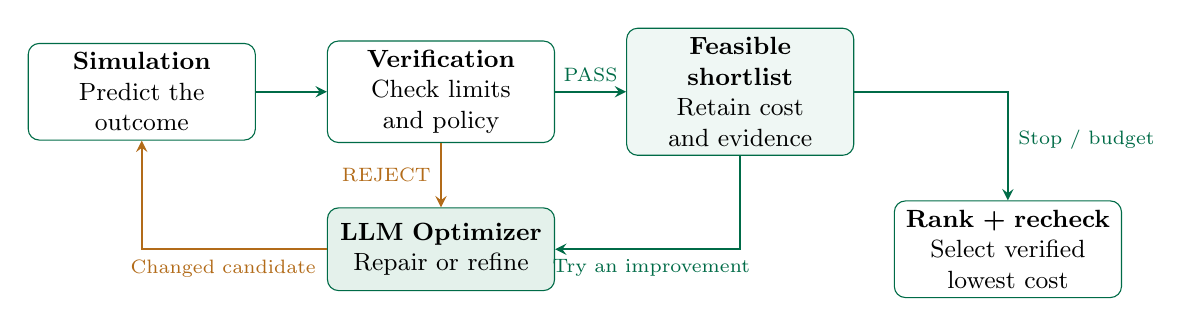
\begin{tikzpicture}[box/.style={draw=forest,rounded corners,align=center,text width=2.65cm,minimum height=1.05cm,font=\small},flow/.style={->,>=stealth,thick,forest}]
\node[box] (model) at (0,0) {\textbf{Simulation}\\Predict the outcome};
\node[box] (gate) at (3.8,0) {\textbf{Verification}\\Check limits and policy};
\node[box,fill=mint!20] (pool) at (7.6,0) {\textbf{Feasible shortlist}\\Retain cost and evidence};
\node[box,fill=mint!35] (opt) at (3.8,-2.0) {\textbf{LLM Optimizer}\\Repair or refine};
\node[box] (rank) at (11.0,-2.0) {\textbf{Rank + recheck}\\Select verified lowest cost};
\draw[flow] (model.east)--(gate.west);
\draw[flow] (gate.east)--node[above,font=\scriptsize]{PASS}(pool.west);
\draw[flow,orange] (gate.south)--node[left,font=\scriptsize]{REJECT}(opt.north);
\draw[flow] (pool.south)|-node[below,pos=.74,font=\scriptsize]{Try an improvement}(opt.east);
\draw[flow,orange] (opt.west)-|node[below,pos=.28,font=\scriptsize]{Changed candidate}(model.south);
\draw[flow] (pool.east)-|node[right,pos=.72,font=\scriptsize]{Stop / budget}(rank.north);
\end{tikzpicture}
\end{center}
\plainidea{Only accepted candidates enter the ranking. Every changed action returns to simulation and verification.}
\slidetransition{How do we enforce an equal maximum trial budget?}
\sources{SmartGridComm 2026 tutorial proposal, p. 2: repair, refinement and simulation-informed ranking. Executed state machine: \texttt{src/proposal\_workflow.py}.}
\note{Optional historical/detail reference, outside the current 180-minute route. Original notebook IDs and experiment scopes are preserved. Use this after the five-module overview. Awareness and Planning have already produced the initial candidates. Simulation and Verification create candidate-specific evidence. A rejected candidate supplies a reason for repair; an accepted candidate may still have poor objective value and invite refinement. The fifth proposal module handles both branches. Under contract revision 1.1, the first bounded refinement is required when valid tools are available. A later iteration may stop through KEEP_INCUMBENT, an exhausted operation set or the maximum budget. This scheduled first refinement is a shared protocol rule, not a freely selected agent behavior. Call or tool failures still lead to REVIEW. A valid shortlist is ranked, and the chosen action is simulated and verified once more before recommendation. If the process requests review or the final check fails, no recommendation is issued. The older eight named helper responsibilities organize execution and explanation; they do not replace these five core proposal modules. Spoken bridge: How do we enforce an equal maximum trial budget?}
\end{frame}

\begin{frame}[t]{Optimize over tested candidates under the same maximum budget}
\[
\mathcal F_B=\{u\in\mathcal C_B:\ \mathrm{solved}(u),\ g_j(x(u),u)\leq0\ \forall j,\ \mathrm{policy}(u)\},
\qquad
u^\star\in\underset{u\in\mathcal F_B}{\arg\min}\ J(x(u),u).
\]
\small
\begin{tabular}{@{}>{\raggedright\arraybackslash}p{.18\linewidth}>{\raggedright\arraybackslash}p{.74\linewidth}@{}}
$\mathcal C_B,\mathcal F_B$ & Tested search candidates and the subset passing all declared checks. \\
$u,x(u),J$ & Action, simulated state and case-specific cost to minimize. \\
$g_j,j,\mathrm{policy}$ & Engineering-limit residual, check index and permitted-action rules. \\
$B,u^\star$ & Maximum new refinement evaluations; best tested feasible action. \\
\end{tabular}
\medskip
\begin{center}
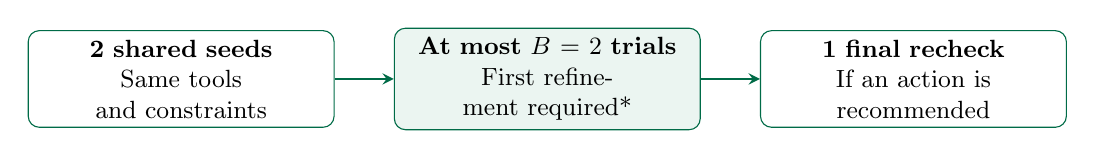
\begin{tikzpicture}[box/.style={draw=forest,rounded corners,align=center,text width=3.65cm,minimum height=.9cm,font=\small},flow/.style={->,>=stealth,thick,forest}]
\node[box] (seeds) at (0,0) {\textbf{2 shared seeds}\\Same tools\\and constraints};
\node[box,fill=mint!25] (refine) at (4.65,0) {\textbf{At most $B=2$ trials}\\First refinement required*};
\node[box] (final) at (9.3,0) {\textbf{1 final recheck}\\If an action is recommended};
\draw[flow] (seeds.east)--(refine.west); \draw[flow] (refine.east)--(final.west);
\end{tikzpicture}
\end{center}
\par\scriptsize *Required when a valid refinement tool is available; later search may stop.\\
Same maximum budget does not imply equal actual evaluations. Report actual counts and elapsed time.\\
Internal MPC solves and the initial state snapshot are additional work, counted separately.
\slidetransition{Which claims belong to the public reason and which to the solver?}
\sources{Finite evaluated-set selection and matched protocol: \texttt{src/proposal\_workflow.py}, \texttt{src/proposal\_case\_tools.py}. Proposal, p. 2: best-of-$N$ and verifier-guided refinement.}
\note{Optional historical/detail reference, outside the current 180-minute route. Original notebook IDs and experiment scopes are preserved. This is a common finite-search formulation, not a guarantee of the global continuous or mixed-integer optimum. The numerical adapters define J, the model and the constraints separately for each physical task. Contract revision 1.1 allows at most two refinement evaluations after two shared seed candidates and requires the first refinement when valid tools are available. Later search may stop early, so actual counts can differ. The fixed and language-guided routes share this rule; the language model chooses among permitted operations rather than freely choosing whether to perform the required first refinement. A failed call or numerical tool can stop with REVIEW. The retained initial contract pilot and revised run must not be pooled as a repeated benchmark. A final independent recheck is outside the search set and is recorded separately; it duplicates the selected physical action and does not add a new optimization candidate. Awareness and MPC preparation can call the electrical model internally, so do not label the four-candidate search cap as a four-power-flow cap. An empty feasible set or held review produces REVIEW. Compare accepted objective values, budget use, failures and full workflow cost, not ticks alone. Spoken bridge: Which claims belong to the public reason and which to the solver?}
\end{frame}

\begin{frame}[t]{The public Llama reason and the numerical evidence have different jobs}
\begin{columns}[T,onlytextwidth]
\begin{column}{.47\textwidth}
\begin{block}{Llama response: interpret the evidence}
\textbf{choice}: one permitted operation.\par\smallskip
\textbf{reason}: a short returned explanation.\par\smallskip
\textbf{ranking}: verified candidate IDs only.
\end{block}
\end{column}
\begin{column}{.49\textwidth}
\begin{block}{Numerical record: check the claim}
Candidate and operating-contract identity.\par\smallskip
Fresh metrics, violations and cost.\par\smallskip
Independent ordering by numerical cost.
\end{block}
\end{column}
\end{columns}
\medskip
\begin{center}
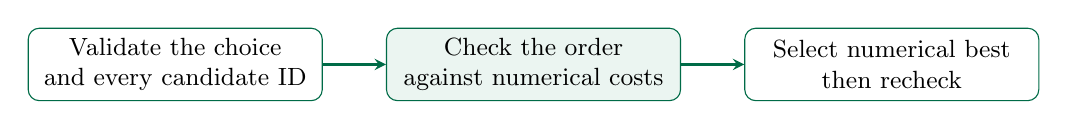
\begin{tikzpicture}[box/.style={draw=forest,rounded corners,align=center,text width=3.5cm,minimum height=.92cm,font=\small},flow/.style={->,>=stealth,thick,forest}]
\node[box] (schema) at (0,0) {Validate the choice\\and every candidate ID};
\node[box,fill=mint!25] (audit) at (4.55,0) {Check the order\\against numerical costs};
\node[box] (choose) at (9.1,0) {Select numerical best\\then recheck};
\draw[flow] (schema.east)--(audit.west); \draw[flow] (audit.east)--(choose.west);
\end{tikzpicture}
\end{center}
\par\small A fluent explanation is a recorded claim. Its supporting measurements and checks remain visible.
\slidetransition{Where is the bounded decision loop implemented?}
\sources{Tool-observation feedback: \href{https://arxiv.org/abs/2210.03629}{Yao et al., ReAct (2023)}. Response validation and ranking guard: \texttt{src/proposal\_workflow.py}.}
\note{Optional historical/detail reference, outside the current 180-minute route. Original notebook IDs and experiment scopes are preserved. No invented model quotation is shown on this concept slide. Later slides display actual returned reason strings and their call IDs. These are public explanations generated by Llama, not hidden internal chain-of-thought and not a physical proof. The shared contract schedules a required first refinement when valid tools are available; Llama chooses its allowed operation, not the existence of every stage. The ranking schema permits every feasible ID exactly once. The implementation records whether Llama's ordering agrees with cost, but numerical minimum cost determines the selected action; language cannot promote a rejected candidate or override the objective. Wrong structure or IDs force review. A cost-order disagreement remains visible for the operator and evaluation rather than being silently presented as correct language reasoning. Latency, token counts, model settings and errors belong to the same trace record. Spoken bridge: Where is the bounded decision loop implemented?}
\end{frame}

\begin{frame}[t]{Initial supervisor code 1/9: a bounded loop controls what can happen next}

\implcode{continuous_workflow}{217}{223}
\footnotesize
\begin{tabular}{@{}>{\raggedright\arraybackslash}p{.22\linewidth}>{\raggedright\arraybackslash}p{.70\linewidth}@{}}
\textbf{Attempt 1} & Validate the shared SAC proposal and request a fresh simulation. \\
\textbf{Attempt 2} & After rejection, check the eligible MPC first action or stop for review. \\
\textbf{Terminal result} & Return a recommendation within the selected model's scope, or return \texttt{REVIEW}. There is no third attempt or equipment command. \\
\end{tabular}
\par\smallskip Both supervisors use the same numerical route and acceptance limits. Llama chooses only a permitted next step.
\slidetransition{How does the operator request become a numerical contract?}
\sources{Executable transition rules: \texttt{src/continuous\_workflow.py}, \texttt{run\_continuous\_workflow}, including lines 252--265. Historical continuous-supervisor protocol 1.1; the new five-stage loop is a separate experiment.}
\note{Optional historical/detail reference, outside the current 180-minute route. Original notebook IDs and experiment scopes are preserved. Optional implementation detail. Begin with the literal range(2), rather than another abstract architecture drawing. The initial planner is allowed VERIFY_SAC_FIRST or REVIEW. After a failed first check, a validated MPC plan can be offered once. A planner REVIEW is terminal for candidate evaluation. Execution here means a numerical proposal, not field dispatch. Ask the audience to locate the two restrictions that prevent arbitrary tool loops: the finite attempt count and the expected tool name. Spoken bridge: How does the operator request become a numerical contract?}
\end{frame}

\begin{frame}[t]{Initial supervisor code 2/9: the request becomes a numerical contract}

\implcode{continuous_workflow}{49}{56}
\footnotesize
\textbf{Units:} voltage is per unit; current allowance is percent of branch rating. For inverter $g$, $S_g$ is kVA, $p_g$ is kW, $q_g$ is kvar, and $a,b$ are dimensionless fleet participation factors.
\par\smallskip\textbf{Authority:} the validated case supplies demand and limits. The language reply has no field for replacing them.
\par\smallskip\textbf{Notebook W2:} inspect this contract before a run. Correct misunderstood operator intent first.
\slidetransition{How do several roles share one local model service?}
\sources{Exact contract: \texttt{src/continuous\_workflow.py}. Case-domain validation and action bounds: \texttt{src/continuous\_control.py}, \texttt{validate\_case} and \texttt{\_control}. Notebook W2.}
\note{Optional historical/detail reference, outside the current 180-minute route. Original notebook IDs and experiment scopes are preserved. Optional. In the current P3 case, rating_fraction is 0.8, so the returned allowance is 80 percent, not an 80 percent reserve. The participation action is shared across the inverter fleet and is not an independently optimized command at every inverter. Contract validation checks form and declared numerical ranges. It does not establish that a request was interpreted correctly or that the sensors are authenticated. This is why readback remains necessary. Spoken bridge: How do several roles share one local model service?}
\end{frame}

\begin{frame}[t]{Initial supervisor code 3/9: named roles share one local Llama service}

\implcode{continuous_workflow}{69}{72}
\implcode{continuous_workflow}{190}{194}
\footnotesize
\textbf{Changes by role:} Planner sees the proposal and contingency plan. Recovery sees failed checks. Explanation sees the metric card. Each receives a restricted menu.
\par\smallskip\textbf{Shared:} one local \texttt{llama3.1:8b} backbone and the numerical tools. Sequential role prompts do not provide independent votes or independent safety assessment.
\par\smallskip The fixed route uses the same interface, so every recorded choice identifies its source.
\slidetransition{How is the language choice restricted to permitted tools?}
\sources{Actual client and role dispatch: \texttt{src/continuous\_workflow.py}. Role/tool interaction background: Yao et al., ReAct (ICLR 2023), \url{https://arxiv.org/abs/2210.03629}.}
\note{Optional historical/detail reference, outside the current 180-minute route. Original notebook IDs and experiment scopes are preserved. Optional. Explain that an agent architecture can impose useful separation of responsibilities without creating statistically independent judgments. This implementation makes no independence claim. One additional role can add another model call and another failure opportunity. The scientific question is whether the resulting interpretation or routing improves a measured task outcome after accounting for errors and cost. Spoken bridge: How is the language choice restricted to permitted tools?}
\end{frame}

\begin{frame}[t]{Initial supervisor code 4/9: the language tool chooses from a restricted menu}

\implcode{continuous_workflow}{75}{78}
\implcode{continuous_workflow}{81}{82}
\footnotesize
\begin{tabular}{@{}>{\raggedright\arraybackslash}p{.20\linewidth}>{\raggedright\arraybackslash}p{.72\linewidth}@{}}
\textbf{Planner menu} & \texttt{VERIFY\_SAC\_FIRST} or \texttt{REVIEW}. Requesting a check does not approve the proposal. \\
\textbf{Recovery menu} & \texttt{USE\_MPC\_PLAN} or \texttt{REVIEW}. The first choice still requires a fresh numerical check. \\
\textbf{Returned reason} & A public explanation of the selected choice, not numerical evidence or a correctness guarantee. \\
\end{tabular}
\slidetransition{Which checks follow valid JSON?}
\sources{Exact schema and system-prompt excerpt: \texttt{src/continuous\_workflow.py}. Structured-response API: \url{https://docs.ollama.com/api/chat}.}
\note{Optional historical/detail reference, outside the current 180-minute route. Original notebook IDs and experiment scopes are preserved. Optional. These excerpts are two separate portions of the actual ask method, not a reconstructed prompt. The call also includes definitions of the permitted actions from CHOICE_DEFINITIONS. The prompt states the policy, while program logic enforces the available routes and numerical gate. A prompt alone cannot establish electrical feasibility. The user-visible reason is stored model output, not a reconstruction of hidden reasoning. Spoken bridge: Which checks follow valid JSON?}
\end{frame}

\begin{frame}[t]{Initial supervisor code 5/9: valid JSON is only the first acceptance test}

\implcode{continuous_workflow}{99}{108}
\footnotesize
\textbf{Established:} two fields, a permitted choice and a nonempty reason. Service, decoding or schema failure produces local \texttt{REVIEW}.
\par\smallskip\textbf{Still unverified:} request semantics, measurement trust, optimality and voltage/current feasibility.
\par\smallskip\textbf{Provenance:} \texttt{actual\_local\_llama} is a parsed reply; \texttt{local\_failure\_fallback} is locally generated text. Neither proves physical safety.
\slidetransition{How does a passing result retain its model scope?}
\sources{Exact parser, fallback and client timer: \texttt{src/continuous\_workflow.py}. Response-source labels are returned at lines 112--114. API response structure: \url{https://docs.ollama.com/api/chat}.}
\note{Optional historical/detail reference, outside the current 180-minute route. Original notebook IDs and experiment scopes are preserved. Optional. The exception path is part of the workflow, not an LLM response. It must not be reported as successful model reasoning. Give the concrete counterexample from the intake study: a perfectly valid structured reply can misread a current reserve. A physical solver operating under that incorrect limit cannot recover the original human intent. The current numerical workflow receives an already approved structured case. Spoken bridge: How does a passing result retain its model scope?}
\end{frame}

\begin{frame}[t]{Initial supervisor code 6/9: a passing result always carries its model scope}

\implcode{continuous_workflow}{273}{278}
\footnotesize
\begin{tabular}{@{}>{\raggedright\arraybackslash}p{.22\linewidth}>{\raggedright\arraybackslash}p{.70\linewidth}@{}}
\textbf{OpenDSS} & Full supplied unbalanced MV/LV feeder. The experiment does not model protection coordination or transients. \\
\textbf{LinDistFlow3} & Coupled MV phase network with idealized LV aggregation. Internal LV voltage/current constraints are omitted. \\
\textbf{Both} & Fresh selected-model simulation, not field evidence or coverage of omitted equipment. \\
\end{tabular}
\par\smallskip\texttt{MODEL\_RECOMMEND} is scoped to the selected model. Different constraint coverage can produce different actions.
\slidetransition{What can a fresh solve reject that prose cannot detect?}
\sources{Exact returned scope: \texttt{src/continuous\_workflow.py}. Model assumptions: \texttt{src/lindistflow3.py} and \texttt{appendix/Stage\_Methods\_and\_Models.md}. Current recorded comparison: \texttt{results/continuous\_workflow\_comparison.json}.}
\note{Optional historical/detail reference, outside the current 180-minute route. Original notebook IDs and experiment scopes are preserved. Optional. Tie this source excerpt to the current P3 example: the MV model accepts the common SAC action, while full AC requires an MPC fallback. This does not establish that the linear MV prediction is inaccurate on the MV buses. It demonstrates why a result must expose its coverage. Plan-level screening also checks that the stored plan backend matches the selected backend. Fresh checking reuses the selected physical model, so it is not independent model validation. Spoken bridge: What can a fresh solve reject that prose cannot detect?}
\end{frame}

\begin{frame}[t]{Initial supervisor code 7/9: a fresh solve can reject a plausible proposal}

\implcode{continuous_workflow}{230}{237}
\footnotesize
\textbf{Inputs:} proposed $[a,b]$, first forecast demand multiplier and approved current allowance. The backend returns fresh action-specific evidence.
\par\smallskip\textbf{Gate:} finite, identified voltage/current arrays, convergence, scope and dispatch tracking. Missing or invalid evidence rejects.
\par\smallskip\textbf{Recovery:} exceptions and mismatches reject. An eligible MPC fallback passes through this same solve and gate.
\slidetransition{How does the code preserve the operator review boundary?}
\sources{Exact fresh-evaluation path: \texttt{src/continuous\_workflow.py}. Deterministic checks: \texttt{src/continuous\_control.py}, \texttt{verify\_control}. Here $a,b$ are dimensionless inverter participation factors.}
\note{Optional historical/detail reference, outside the current 180-minute route. Original notebook IDs and experiment scopes are preserved. Optional. Emphasize the difference between the model's own accepted flag and the deterministic gate that reconstructs the checks from the returned arrays. The checker requires nonempty finite data, identities, fresh convergence, valid scope, the requested case, voltage and current bounds, and actual versus commanded P/Q tracking. This is a first-action check. The MPC plan has separate horizon evidence, and neither proves stability or robustness to unknown disturbances. Spoken bridge: How does the code preserve the operator review boundary?}
\end{frame}

\begin{frame}[t]{Initial supervisor code 8/9: the final authority stays with the operator}

\implcode{continuous_workflow}{61}{64}
\implcode{continuous_workflow}{288}{291}
\footnotesize
\textbf{Read back:} proposed P/Q, participation factors, current allowance and scope. Review measurement, protection and implementation questions.
\par\smallskip\textbf{Record identity:} the hash binds the decision fields to this record. Local acknowledgment neither dispatches equipment nor overrides rejection.
\par\smallskip\textbf{Benefit to test:} consistent evidence for human review. Operator workload and live ADMS deployment are not evaluated.
\slidetransition{Which saved call produced the displayed response?}
\sources{Exact local-review contract: \texttt{src/continuous\_workflow.py}. Human/automation allocation background: Parasuraman, Sheridan and Wickens (2000), \url{https://doi.org/10.1109/3468.844354}. Dashboard checkpoint F2.}
\note{Optional historical/detail reference, outside the current 180-minute route. Original notebook IDs and experiment scopes are preserved. Optional. The operator remains a person, not another Llama role. The final dashboard is local and has no SCADA dispatch API. Hashing supports record identity but does not authenticate the human, sensors, model or source files. A future operational integration would need separate authority and assurance work. Ask the audience which displayed quantity would reveal a mistaken interpretation of a 20 percent current reserve. Spoken bridge: Which saved call produced the displayed response?}
\end{frame}

\begin{frame}[t]{Initial supervisor code 9/9: match the displayed response to its recorded call}

\checkpoint{T1}{Open the read-only trace notebook and load the supplied evidence.}
\implcode{continuous_workflow}{108}{114}
\footnotesize
\textbf{Stage record:} the role, numerical method, status, response source and returned content travel together. The journal retains the actual request context and raw local-model response.
\par\smallskip\textbf{Audit rule:} the reader requires the same call ID, choice, reason and recorded client duration. It rejects missing or nonunique matches instead of selecting a convenient journal.
\par\smallskip T2--T6 expose the voltage, MILP, h06 intake and cyber traces. T7--T9 then inspect timing fields and source hashes. Reading these files does not invoke a solver or Llama.
\slidetransition{Which two clocks appear in the recorded trace?}
\sources{Exact stage schema, journal and client timer: \texttt{src/continuous\_workflow.py}. Matching reader: \texttt{src/trace\_latency.py}. Companion: \texttt{Agent\_Trace\_and\_Latency.ipynb}, T1--T9.}
\note{Optional historical/detail reference, outside the current 180-minute route. Original notebook IDs and experiment scopes are preserved. Optional. This is the bridge from architecture to inspectable experiments: every claim on the later case slides should point to a numerical return or an actual recorded language response. The call ID is local to its journal, so the source path and unique matching rule also matter. Deterministic stages do not acquire invented LLM reasons or invented per-stage timings. The notebooks are evidence readers unless the main experiment explicitly launches a live call. Spoken bridge: Which two clocks appear in the recorded trace?}
\end{frame}

\begin{frame}[t]{Trace review 1/3: read token counts and two distinct clocks}

\checkpoint{T7}{Inspect the recorded calls and usage fields.}
\begin{columns}[T,onlytextwidth]
\begin{column}{.61\textwidth}
\includegraphics[width=\linewidth,height=.61\textheight,keepaspectratio]{\figfile{recorded_call_latency_slide.png}}
\end{column}
\begin{column}{.36\textwidth}
\footnotesize
\textbf{Client:} HTTP request, parsing and schema validation, timed in seconds.
\par\smallskip\textbf{Server:} \texttt{total\_duration} converted from nanoseconds. Do not add it to client time.
\par\smallskip\textbf{Tokens:} \texttt{prompt\_eval\_count} (input), \texttt{eval\_count} (output).
\par\smallskip\textbf{Example, current AC Planner:} 795 input tokens, 36 output tokens, 0.988 s client and 0.955 s server.
\par\smallskip Unmeasured stage times and causes stay unknown.
\end{column}
\end{columns}
\slidetransition{How does measured cost relate to the actual outcome?}
\sources{Matched raw journals read by \texttt{src/trace\_latency.py}, \texttt{\_call\_row}. API field units: \url{https://docs.ollama.com/api/chat}. Figure: three current OpenDSS calls; T7 includes all ten selected calls.}
\note{Optional historical/detail reference, outside the current 180-minute route. Original notebook IDs and experiment scopes are preserved. Optional. Explain that token throughput, if inspected in the table, is output count divided by eval_duration converted to seconds. It is a generation-rate measure, not total application throughput. For the current AC Planner this is about 74.3 generated tokens per second. Do not infer network overhead, queueing, hardware effects or cache causality from the difference of these aggregate intervals. The h06 client call is distinct from its slightly longer intake wrapper, and its downstream numerical runtime is a third interval. Spoken bridge: How does measured cost relate to the actual outcome?}
\end{frame}

\begin{frame}[t]{Trace review 2/3: compare cost with the recorded outcome}

\checkpoint{T8}{Compare fixed and agentic intervals within each recorded pair.}
\begin{columns}[T,onlytextwidth]
\begin{column}{.64\textwidth}
\includegraphics[width=\linewidth,height=.62\textheight,keepaspectratio]{\figfile{recorded_workflow_latency_slide.png}}
\end{column}
\begin{column}{.33\textwidth}
\footnotesize
\textbf{Fixed / agentic seconds}\par
AC: 0.346 / 3.110 s.\par
MV: 0.134 / 4.911 s.\par
Same action within each backend.
\par\smallskip\textbf{Historical cases}\par
MILP: 0.009859 / 6.10178 s.\par
Cyber: 0.002146 / 5.93465 s.\par
Checks pass; the agentic explanation returns \texttt{REVIEW}.
\par\smallskip\textbf{No speed gain.} Language calls add time and can add unnecessary handoffs.
\end{column}
\end{columns}
\par\footnotesize Current: precomputed controllers/training excluded. Historical: numerical tools included. One run per route; h06 at T5.
\slidetransition{What should the next controlled study measure?}
\sources{Records: \texttt{results/workshop\_run\_[backend].json}, \texttt{standard\_agent\_workflow.json}. Interval definitions: \texttt{src/trace\_latency.py}.}
\note{Optional historical/detail reference, outside the current 180-minute route. Original notebook IDs and experiment scopes are preserved. Optional. These are descriptive observations on one machine, not matched repeated statistical benchmarks. Compare fixed and agentic within each recorded pair, but do not pool protocols or rank backend speed from differently timed runs. The difference between total workflow time and summed client calls is only other work inside that interval, not a measured solver-stage timer. The positive h06 intake example demonstrates language coverage with errors elsewhere in the study; it does not turn these timing results into a speed advantage. Spoken bridge: What should the next controlled study measure?}
\end{frame}

\begin{frame}[t]{Trace review 3/3: audit this record; design the next study}

\checkpoint{T9}{Inspect the source hashes and evidence audit.}
\cellcode{T9}{1}{5}
\footnotesize
\begin{tabular}{@{}>{\raggedright\arraybackslash}p{.24\linewidth}>{\raggedright\arraybackslash}p{.68\linewidth}@{}}
\textbf{What this audit proves} & Matches specific saved bytes and replies. A hash detects change against a retained reference. \\
\textbf{What it cannot prove} & Truth, model adequacy, operator identity or general performance. Recomputed hashes do not authenticate sources. \\
\textbf{Next matched study} & Freeze cases, limits, models, prompts and code. Repeat both routes with declared seeds and randomized order. \\
\textbf{Measure together} & Correctness, acceptance, unnecessary review, failures and time. Separate cold/warm setup and measure operator outcomes. \\
\end{tabular}

\slidetransition{How are the three phases coupled in the linear approximation?}
\sources{Exact source hashing: \texttt{src/trace\_latency.py}. Raw-source hashes and unique journal matching are returned by \texttt{load\_recorded\_evidence}. Companion T9 records the files actually inspected.}
\note{Optional historical/detail reference, outside the current 180-minute route. Original notebook IDs and experiment scopes are preserved. Optional. There are eight source files in the current evidence collection, but the count is not hard-coded here so the notebook remains authoritative if packaging adds records. Store an external trusted reference if authenticity matters. Distinguish a file hash from the recommendation-field hash used by the dashboard. For a repeated experiment, predeclare handling of timeouts, failed schemas, incorrect READY replies and correct abstentions. Do not silently drop slow calls or failed tasks before reporting latency. This page proposes future methodology; it claims no new measurements. Spoken bridge: How are the three phases coupled in the linear approximation?}
\end{frame}

\begin{frame}[t]{Optional reference: coupled three-phase LinDistFlow}
\referencefont
\[
S_{ij}=s_j+\sum_{k:j\to k}S_{jk},\qquad
w_j=w_i-2\operatorname{Re}\{\overline D_\beta Z_{ij}D_\beta\overline S_{ij}\}.
\]
\referencefont
\begin{tabular}{@{}>{\raggedright\arraybackslash}p{.24\linewidth}>{\raggedright\arraybackslash}p{.69\linewidth}@{}}
\toprule Symbol / domain & Meaning and units \\
\midrule
$i,j,k$; $j\to k$ & Parent bus, child bus and downstream child; sum over the outgoing branches of bus $j$. \\
$S_{ij}\in\mathbb C^{n_\phi}$ & Branch phase powers $P_{ij}+\mathrm{i}Q_{ij}$ in VA (real parts W, imaginary parts var); $n_\phi$ is the branch's number of present phases. \\
$s_j\in\mathbb C^{n_\phi}$ & Net complex consumption at bus $j$, positive for consumption and negative for injection, in VA. \\
$w_i,w_j\in\mathbb R_+^{n_\phi}$ & Squared phase-to-neutral voltage magnitudes $|V|^2$, in V$^2$; the solver later converts magnitudes to per unit. \\
$Z_{ij}\in\mathbb C^{n_\phi\times n_\phi}$ & Phase impedance matrix in $\Omega$, including mutual impedances. \\
$D_\beta=\operatorname{diag}(\beta)$ & Nominal phase ratios $\beta=(1,e^{-\mathrm{i}2\pi/3},e^{\mathrm{i}2\pi/3})$ restricted to present phases; dimensionless. \\
$\overline{(\cdot)},\operatorname{Re},\mathrm{i}$ & Complex conjugation, componentwise real part, and imaginary unit $\mathrm{i}^2=-1$. \\
\bottomrule
\end{tabular}
\par\smallskip\textbf{Assumptions:} radial energized topology; nearly nominal phase-angle ratios; series-loss terms omitted in the balance. Balance terms use a common bus-phase ordering with absent phases zero-filled; voltage drop uses present branch phases. The export aggregates LV injections and omits internal LV constraints.
\slidetransition{How do objective terms and constraints define voltage support?}
\sources{Gan and Low (2014), Sec. V, \url{https://arxiv.org/abs/1406.3054}. Export and implementation: \texttt{src/lindistflow3.py}.}
\note{Optional historical/detail reference, outside the current 180-minute route. Original notebook IDs and experiment scopes are preserved. Optional, outside the three-hour timing. Explain dimensions before the multiplication: ohms times VA gives volts squared. The displayed equation uses physical units; multiplying kVA directly by ohms without converting would be wrong. The real-part expression retains phase coupling. Approximate reported losses are separate from the lossless balance. Model coverage, approximation error and solver convergence are different questions. Spoken bridge: How do objective terms and constraints define voltage support?}
\end{frame}

\begin{frame}[t]{Optional reference: voltage-control objective and constraints}
\referencefont
\[
\min_{x_k,u_k}\sum_{k,i,\phi}w_v(v_{i\phi,k}-v^{\rm ref})^2
+\sum_{k,g}\big[w_p(p^{\rm av}_{g,k}-p_{g,k})^2+w_q q_{g,k}^2\big]
\]
\[
F_m(x_k,u_k;\hat d_k)=0,\quad \underline v\leq v\leq\overline v,\quad
|I|\leq\overline I,\quad 0\leq p_g\leq p_g^{\rm av},\quad p_g^2+q_g^2\leq S_g^2.
\]
\referencefont
\begin{tabular}{@{}>{\raggedright\arraybackslash}p{.25\linewidth}>{\raggedright\arraybackslash}p{.68\linewidth}@{}}
$k,i,\phi,g$ & Time-step, bus, available-phase and PV-inverter indices. Sums cover the modeled horizon, bus phases and inverters. \\
$x_k\in\mathbb R^{n_x},u_k\in\mathbb R^{2n_g}$ & Real representation of electrical states and inverter P/Q controls; $n_x$ is the state dimension and $n_g$ the inverter count. \\
$F_m,\hat d_k$ & Selected model $m$'s power-flow residual and forecast active/reactive demand (kW/kvar). Zero residual imposes its electrical equations. \\
$v,v^{\rm ref},\underline v,\overline v$ & Voltage magnitude, target and bounds in pu; $I,\overline I$ are phase-current magnitude and allowed limit in A. Inequalities are componentwise. \\
$p_g,p_g^{\rm av},q_g,S_g$ & Active output/availability (kW), reactive output (kvar), apparent rating (kVA). \\
$w_v,w_p,w_q\geq0$ & Objective weights; their units or input normalization must make the summed objective consistent. \\
\end{tabular}
\par\smallskip\textbf{Executed snapshot reduction:} $p_g=aS_g$, $q_g=bS_g$ with dimensionless $a\in[0,1]$, $b\in[-.44,.44]$ and $a^2+b^2\leq1$. It minimizes the dimensionless cost $(1-a)^2+.05b^2+10\operatorname{mean}[(v-1.01)^2]$ across modeled voltage entries.
\slidetransition{What exactly is the implemented finite-horizon plan?}
\sources{Maharjan et al. (2021), \url{https://doi.org/10.1109/TSTE.2020.3001115}. Restricted snapshot: \texttt{src/standard\_formulations.py}.}
\note{Optional historical/detail reference, outside the current 180-minute route. Original notebook IDs and experiment scopes are preserved. Optional. The first equations describe a general problem; the final paragraph defines the actual two-variable reduction. Available P equals rated S only under the supplied high-irradiance overlay. A sequential local sensitivity solve, inscribed capability polygon and fresh checks do not provide global AC optimality. The general model can be extended to individual inverter decisions, but that larger optimization was not executed here. Spoken bridge: What exactly is the implemented finite-horizon plan?}
\end{frame}

\begin{frame}[t]{Optional reference: the executed continuous horizon plan}
\referencefont
\[
\min_{u_0,u_1,u_2}\sum_{k=0}^{2}\gamma^k\ell_k,\quad
\ell_k=(1-a_k)^2+.05b_k^2+\frac{10}{N_v}\sum_{r=1}^{N_v}(v_{r,k}-1.01)^2
+.05\|u_k-u_{k-1}\|_2^2.
\]
\referencefont
\begin{tabular}{@{}>{\raggedright\arraybackslash}p{.25\linewidth}>{\raggedright\arraybackslash}p{.68\linewidth}@{}}
\toprule Symbol / value & Meaning and implementation \\
\midrule
$H=3$, $k\in\{0,1,2\}$ & Three forecast steps. No physical step duration or dynamic energy state is specified in this quasistatic teaching model. \\
$u_k=(a_k,b_k)\in\mathbb R^2$ & Dimensionless fleet participation; $p_g=a_kS_g$ kW and $q_g=b_kS_g$ kvar for inverter rating $S_g$ in kVA. \\
$u_{-1}$ & Declared previous fleet command; the Euclidean squared norm penalizes changes from it or from the preceding planned step. \\
$v_{r,k}$; $N_v$ & Per-unit voltage magnitude at modeled bus-phase entry $r$; number of such entries in the selected model. \\
$\gamma=.98$, $\ell_k$ & Dimensionless discount and dimensionless engineering stage cost. Numeric coefficients are declared teaching weights, not fitted monetary costs. \\
$\rho\in(0,1]$ & Permitted nominal-current fraction: each predicted phase current must satisfy $|I|\leq\rho I^{\rm rated}$ (A). \\
\bottomrule
\end{tabular}
\par\smallskip\textbf{Algorithm:} rebuild local voltage/current sensitivities, solve a constrained QP step, and retain only a nonincreasing-cost horizon passing fresh model checks. The 32-sided inscribed capability polygon is conservative. The tool proposes $u_0$; this study inspects a horizon decision rather than an executed closed-loop rollout of MPC.
\slidetransition{How do policy outputs map to physical inverter controls?}
\sources{Rawlings, Mayne and Diehl, \emph{Model Predictive Control}, 2nd ed. (2017), \url{https://sites.engineering.ucsb.edu/~jbraw/mpc/}. Executed plan: \texttt{src/continuous\_control.py}.}
\note{Optional historical/detail reference, outside the current 180-minute route. Original notebook IDs and experiment scopes are preserved. Optional. Six real control variables are optimized. The three forecast loads and movement penalty couple the stages, but storage dynamics are absent. Fresh horizon feasibility is tool evidence; the common workflow gate checks the chosen first action. There is no recursive-feasibility, stability, uncertainty-robustness or global-optimality certificate. A small voltage-objective value on an MV-only model cannot certify LV service voltage. Spoken bridge: How do policy outputs map to physical inverter controls?}
\end{frame}

\begin{frame}[t]{Optional reference: SAC objective, action mapping and reward}
\setlength{\parskip}{0pt}
\referencefont
\setlength{\abovedisplayskip}{0pt}\setlength{\belowdisplayskip}{1pt}\setlength{\abovedisplayshortskip}{0pt}\setlength{\belowdisplayshortskip}{1pt}
\[
\max_\pi\;\mathbb E_\pi\!\left[\sum_{t=0}^{2}\gamma^t\{r_t+\alpha\mathcal H(\pi(\cdot\mid o_t))\}\right],\quad
a=\tfrac12(z_1+1),\quad b=z_2\min\{.44,\sqrt{1-a^2}\}.
\]
\[
r_t=-\ell_t-40(e_v/.05)^2-10e_I^2-2\mathbf1\{e_v>0\text{ or }e_I>0\}.
\]
\[
e_v=[.95-\hat v_{\min}]_++[\hat v_{\max}-1.05]_+,\qquad e_I=[\hat\iota-1]_+.
\]
\referencefont
\begin{tabular}{@{}>{\raggedright\arraybackslash}p{.24\linewidth}>{\raggedright\arraybackslash}p{.69\linewidth}@{}}
$\pi$; $z\in[-1,1]^2$; $a,b$ & Policy, normalized action with components $z_1,z_2$, and dimensionless fleet P/Q participation. Evaluation uses tanh of the Gaussian mean before mapping. \\
$o_t\in\mathbb R^7$ & Three forecast demand multipliers, previous $a,b$, allowed current fraction, remaining horizon/3; all dimensionless. \\
$\mathbb E_\pi,\mathcal H,\alpha=.005$ & Expectation under the policy/environment; differential entropy in normalized action coordinates (natural logarithm); fixed entropy coefficient. \\
$t,\gamma=.98,r_t,\ell_t$ & Training step, discount, reward and engineering cost. Training predicts its voltage-MSE term directly with the fitted response surface. Reward/cost are dimensionless. \\
$e_v,\hat v_{\min},\hat v_{\max}$ & Voltage excess and predicted minimum/maximum voltage, in pu. A hat denotes a fitted response; $[x]_+=\max(x,0)$. \\
$e_I,\hat\iota$ & Dimensionless current excess and predicted maximum line-phase current/rating ratio. Each line-phase uses its own rating; training fixes allowed fraction $\rho=1$. \\
$\mathbf1\{\cdot\}$ & Indicator: one when any stated surrogate violation occurs, zero otherwise. \\
\end{tabular}
\par\textbf{Protocol:} seed 23; 12,000 reward-only transitions; two 64-unit hidden layers; no MPC labels. Fresh network checks remain necessary.
\slidetransition{Which restoration variables enforce service and radiality?}
\sources{Haarnoja et al. (2018), \url{https://proceedings.mlr.press/v80/haarnoja18b.html}. Protocol: \texttt{models/continuous\_sac/training\_protocol.json}; optional \texttt{Continuous\_SAC\_Training.ipynb}.}
\note{Optional historical/detail reference, outside the current 180-minute route. Original notebook IDs and experiment scopes are preserved. Optional. The entropy coefficient is fixed, not automatically learned. The actor and critic optimize the declared surrogate environment. Training return, fit-validation error and fresh physical evaluation are different evidence sets. The action map enforces the device circle but cannot enforce voltage or line-current constraints. The nominal current used in the training penalty is intentional; it makes the reserve case a distribution shift. Spoken bridge: Which restoration variables enforce service and radiality?}
\end{frame}

\begin{frame}[t]{Optional reference: restoration MILP variables and topology}
\setlength{\abovedisplayskip}{3pt}\setlength{\belowdisplayskip}{3pt}\setlength{\parskip}{0pt}
\referencefont
\[
\max\sum_{i\ne0}w_iP_i^d s_i,\quad s_i\leq y_i,\quad
-\overline P_{ij}z_{ij}\leq P_{ij}\leq\overline P_{ij}z_{ij},\quad
\sum_jP_{ji}-\sum_jP_{ij}=P_i^d s_i\quad(i\ne0).
\]
\[
\sum_j f_{ji}-\sum_j f_{ij}=y_i\quad(i\ne0),\quad |f_{ij}|\leq5z_{ij},\quad
\sum_{(i,j)\in E}z_{ij}=\sum_{i\in N}y_i-1.
\]
\referencefont
\renewcommand{\arraystretch}{.98}
\begin{tabular}{@{}>{\raggedright\arraybackslash}p{.25\linewidth}>{\raggedright\arraybackslash}p{.68\linewidth}@{}}
$N,E,i,j$ & Fixture's six buses and candidate edges, with source bus $0$; each edge has one arbitrary reference orientation. Signed flows may oppose it. \\
$s_i,y_i,z_{ij}\in\{0,1\}$ & Load picked up, bus energized, and branch energized. $s_i\leq y_i$ permits an energized transit bus with its load disconnected. \\
$P_i^d\geq0,\overline P_{ij}\geq0,P_{ij}\in\mathbb R$ & Demand, branch capacity and signed active flow, all in kW. Source export equals total picked-up demand. \\
$w_i>0$ & Dimensionless service weight: 10 for the two critical loads, 1 otherwise. The objective is weighted kW; finite weights are not lexicographic priority. \\
$f_{ij}\in\mathbb R$ & Dimensionless connectivity commodity; each energized non-source bus consumes one unit. Source exports $\sum_{i\ne0}y_i$; 5 bounds its total. \\
$y_0=1$, $z_{ij}\leq y_i,y_j$ & Source remains energized; an energized edge requires energized endpoints. Unavailable edges have $z_{ij}=0$. \\
\end{tabular}
\par\textbf{Why radial:} connectivity plus the displayed edge count enforces a tree; edge count alone permits disconnected cycles. A second solve fixes weighted service and minimizes energized branch count.
\slidetransition{How is the residual statistic calibrated?}
\sources{Chen et al. (2018), \url{https://doi.org/10.1109/TPWRS.2017.2720122}; Wang et al. (2020), \url{https://arxiv.org/abs/1912.05185}. This is the six-node active-power fixture, not the feeder catalog.}
\note{Optional historical/detail reference, outside the current 180-minute route. Original notebook IDs and experiment scopes are preserved. Optional. The balance sign follows the chosen edge orientation, with outgoing flow subtracted from incoming flow at non-source buses. Binary y, s and z have different meanings. Edge count alone would permit a disconnected cycle; the commodity constraints exclude it. Capacity is active power here, not a three-phase thermal calculation. The secondary objective is not switch operations from a prior topology. Spoken bridge: How is the residual statistic calibrated?}
\end{frame}

\begin{frame}[t]{Optional reference: WLS, residual covariance and calibration}
\referencefont
\[
\hat x=\arg\min_{x\in\mathbb R^n}(z-Hx)^\top R^{-1}(z-Hx),\quad r=z-H\hat x,
\quad\Omega=R-H(H^\top R^{-1}H)^{-1}H^\top.
\]
\[
r_i^N=|r_i|/\sqrt{\Omega_{ii}},\qquad J=r^\top R^{-1}r,\qquad
J>\chi^2_{m-n,\,1-\alpha}\ \Longrightarrow\ \text{residual alarm}.
\]
\referencefont
\begin{tabular}{@{}>{\raggedright\arraybackslash}p{.23\linewidth}>{\raggedright\arraybackslash}p{.70\linewidth}@{}}
$x,\hat x\in\mathbb R^n$ & True and estimated non-source voltage angles (radians), $n=3$ in the four-bus DC fixture. \\
$z\in\mathbb R^m,H\in\mathbb R^{m\times n}$ & $m=8$ measurements and their linear map: four branch flows, three injections (pu), and one angle (rad). Each row of $H$ maps rad to that channel's units. \\
$R\succ0,\Omega\in\mathbb R^{m\times m}$ & Noise and residual covariance matrices, with channel-dependent squared/cross units. $R$ is diagonal for the stated independent noise. \\
$r,r_i,r_i^N$ & Residual vector, its channel $i$ component in native units, and dimensionless normalized magnitude. Defined only for $\Omega_{ii}>0$. \\
$J,\chi^2_{\nu,1-\alpha},\nu=m-n$ & Dimensionless weighted residual statistic, chi-square quantile and degrees of freedom; $\alpha=.01$, $\nu=5$, threshold 15.0863. \\
$\top$, $R^{-1}$ & Matrix transpose and inverse. Implementation uses weighted least squares/linear solves; the inverse notation states the mathematics. \\
\end{tabular}
\par\smallskip\textbf{Calibration assumptions:} correct linear model, full column rank $\operatorname{rank}(H)=n$, and Gaussian noise with the stated covariance. A residual alarm signals inconsistency; it does not identify malicious intent. Recheck rank after removing a channel.
\slidetransition{Why can a coordinated corruption leave the residual unchanged?}
\sources{Schweppe and Wildes (1970), \url{https://doi.org/10.1109/TPAS.1970.292678}; Handschin et al. (1975), \url{https://doi.org/10.1109/T-PAS.1975.31858}.}
\note{Optional historical/detail reference, outside the current 180-minute route. Original notebook IDs and experiment scopes are preserved. Optional. Distinguish m measurements from n unknown states, and explain whitening through R. The displayed alpha is a nominal false-alarm probability under the stated model, not a measured attack-detection rate. The largest normalized residual is a localization heuristic. Zero residual variance gives an undefined normalized statistic, and a rank-deficient retained set does not support the same estimator. Spoken bridge: Why can a coordinated corruption leave the residual unchanged?}
\end{frame}

\begin{frame}[t]{Optional reference: why a coordinated corruption can be invisible}
\referencefont
\[
z'=z+Hc,\qquad \hat x'=\hat x+c,\qquad z'-H\hat x'=z-H\hat x=r.
\]
\referencefont
\begin{tabular}{@{}>{\raggedright\arraybackslash}p{.25\linewidth}>{\raggedright\arraybackslash}p{.68\linewidth}@{}}
\toprule Symbol / domain & Meaning in the fixed linear WLS model \\
\midrule
$z,z'\in\mathbb R^m$ & Original and corrupted measurement vectors, retaining each channel's native units. \\
$H\in\mathbb R^{m\times n}$ & Known, unchanged full-column-rank measurement matrix; here $m=8,n=3$. \\
$c\in\mathbb R^n$ & Attacker's selected angle shift (rad). The added measurement vector $Hc$ has the correct units for every channel. \\
$\hat x,\hat x'\in\mathbb R^n$ & Original and shifted state estimates (rad); $r$ is their identical residual in measurement units. \\
$\mathcal T,H_{\mathcal T}$ & Index set of protected measurement channels and the corresponding rows of $H$. \\
\bottomrule
\end{tabular}
\par\medskip If protected channels cannot change, a corruption of this form must satisfy $H_{\mathcal T}c=0$. When $H_{\mathcal T}$ has full column rank, only $c=0$ is possible within this attack construction.
\par\medskip\textbf{Threat assumptions:} the attacker knows $H$ and can modify every unprotected channel required by $Hc$. This does not establish that an arbitrary attacker can create the same effect. A low residual does not reject consistency under the stated model; it does not establish the truth of the measurements.
\slidetransition{How does protected information enter constrained control?}
\sources{Liu, Ning and Reiter (2009), \url{https://doi.org/10.1145/1653662.1653666}. Exact fixture: \texttt{src/standard\_formulations.py}, \texttt{run\_wls\_demo}.}
\note{Optional historical/detail reference, outside the current 180-minute route. Original notebook IDs and experiment scopes are preserved. Optional. Substitute the shifted estimate directly into the residual and cancel Hc. This exact cancellation is a property of this linear model with an unchanged matrix, not a blanket statement about nonlinear AC state estimation. The protected-set rank argument rules out this particular Hc shift when the stated channels are trustworthy; it does not authenticate channels or address every attack class. Spoken bridge: How does protected information enter constrained control?}
\end{frame}

\begin{frame}[t]{Optional reference: trusted-data estimation and constrained control}
\referencefont
\[
H_{\mathcal T}=I_3,\quad
b=FB^{-1}e_2,\qquad
\min_{0\leq u\leq .5}\tfrac12u^2
\quad\text{s.t.}\quad |F\hat x_{\mathcal T}+bu|\leq\overline f-.01\mathbf1.
\]
\referencefont
\begin{tabular}{@{}>{\raggedright\arraybackslash}p{.25\linewidth}>{\raggedright\arraybackslash}p{.68\linewidth}@{}}
$\mathcal T,H_{\mathcal T},I_3$ & Three assumed trustworthy angle channels, their measurement matrix, and the $3\times3$ identity. Additional independent angle channels make the toy state observable; this identity is not a row subset of the original eight-channel matrix. \\
$\hat x_{\mathcal T}\in\mathbb R^3$ & Estimate from protected angles, in rad. Three measurements minus three states leave zero residual-test degrees of freedom. \\
$u\in[0,.5]$ & Flexible active injection at bus 2, in pu, balanced by the source. The dimensionless quadratic cost selects the smallest feasible injection. \\
$F\in\mathbb R^{4\times3},B\in\mathbb R^{3\times3}$ & DC maps from non-source angles to branch flows and nodal injections; entries convert rad to pu power. \\
$e_2=(0,1,0)^\top$, $b\in\mathbb R^4$ & Unit selector of bus-2 injection and induced branch-flow change per unit injection. \\
$\overline f=(.35,.18,.35,.35)^\top$ & Absolute branch-flow limits in pu for branches 01, 12, 23, 03. $\mathbf1\in\mathbb R^4$ is an all-ones vector. \\
$F\hat x_{\mathcal T}+bu$, $.01$ & Predicted branch flows and declared planning margin, both in pu; absolute value and inequality act per branch. \\
\end{tabular}
\par\smallskip\textbf{Check after solving:} verify finite values, $u$ bounds and predicted constraints; then evaluate the action against the known synthetic true state. Protected-data control removes the toy overload, subject to the assumed channel trust. The margin is not a calibrated uncertainty bound.
\slidetransition{Which assumptions still limit the scientific claim?}
\sources{Estimation/attack context: \url{https://doi.org/10.1109/TPAS.1970.292678}; \url{https://doi.org/10.1145/1653662.1653666}. Constrained DC teaching response: \texttt{src/standard\_formulations.py}.}
\note{Optional historical/detail reference, outside the current 180-minute route. Original notebook IDs and experiment scopes are preserved. Optional. F and B use the fixture's signed branch-incidence convention; using the same convention in both yields the action sensitivity b. The decision is a scalar DC injection, not feeder-wide AC cyber recovery. Synthetic truth is available to the evaluator, not to an actual operator. The trusted set is an explicit premise, and Llama cannot establish it. Spoken bridge: Which assumptions still limit the scientific claim?}
\end{frame}

\begin{frame}[t]{Study boundaries and the next scientific comparisons}
\referencefont
\begin{tabular}{@{}>{\raggedright\arraybackslash}p{.27\linewidth}>{\raggedright\arraybackslash}p{.66\linewidth}@{}}
\toprule Record & What it measures \\
\midrule
Proposal-complete suite & Six settings $\times$ two supervisors; 24 Llama calls, plus one separate four-call Qwen example. One disclosed development revision; five cost ties and one worse Llama outcome. \\
Initial workshop runs & Continuous SAC/MPC proposals, checks and local Llama fallback choices under both model backends. \\
Language confirmation & 12 authored requests; 8 clear and 4 requiring clarification, with independent semantic scoring and the same downstream tools. \\
SAC training & 12,000 nominal-domain interactions; six authored model/case evaluations. One training seed does not quantify algorithm variability. \\
Standard-method traces & One permitted numerical attempt around continuous P/Q, a six-node MILP or four-bus DC WLS recovery. \\
Historical 32-run corpus & Eight finite-catalog feeder fixtures, two model backends, two supervisors and separate AC reference audits. \\
\bottomrule
\end{tabular}
\par\smallskip\referencefont Language confirmation: correct completion $5/8$ for the parser and $7/8$ for selective Llama; wrong READY interpretations $1/12$ and $2/12$. Numerators count observed outcomes; denominators are clear requests (8) or all requests (12). The restoration subset does not replace the parent-study result.
\par\smallskip\referencefont\textbf{Next comparison:} predeclare unseen cases, repeat model calls and training seeds, match tool/retry budgets, and report incorrect recommendations separately from correct abstentions. Human time and workload need a separate human study.
\slidetransition{Choose one matched comparison to investigate after class.}
\sources{Study design: \texttt{appendix/Agentic\_Advantage\_Study.md}. Recent benchmark context: Mansutti et al. (2026 preprint), \url{https://arxiv.org/abs/2609.00384}. Reading map: \texttt{appendix/Recent\_Agentic\_AI\_Literature.md}.}
\note{Optional historical/detail reference, outside the current 180-minute route. Original notebook IDs and experiment scopes are preserved. Optional. Keep these experiments separate whenever stating a benefit. A successful tool call, correct intent, physical feasibility, good objective and suitable human review are different outcomes. Nothing here establishes field reliability, globally optimal AC control, an authenticated dispatch system, or human time savings. These denominators and limitations are essential to interpreting the observed Llama results in each lesson. Spoken bridge: Choose one matched comparison to investigate after class.}
\end{frame}

\fi
\end{document}
